\documentclass[twoside]{book}

% Packages required by doxygen
\usepackage{fixltx2e}
\usepackage{calc}
\usepackage{doxygen}
\usepackage[export]{adjustbox} % also loads graphicx
\usepackage{graphicx}
\usepackage[utf8]{inputenc}
\usepackage{makeidx}
\usepackage{multicol}
\usepackage{multirow}
\PassOptionsToPackage{warn}{textcomp}
\usepackage{textcomp}
\usepackage[nointegrals]{wasysym}
\usepackage[table]{xcolor}

% Font selection
\usepackage[T1]{fontenc}
\usepackage[scaled=.90]{helvet}
\usepackage{courier}
\usepackage{amssymb}
\usepackage{sectsty}
\renewcommand{\familydefault}{\sfdefault}
\allsectionsfont{%
  \fontseries{bc}\selectfont%
  \color{darkgray}%
}
\renewcommand{\DoxyLabelFont}{%
  \fontseries{bc}\selectfont%
  \color{darkgray}%
}
\newcommand{\+}{\discretionary{\mbox{\scriptsize$\hookleftarrow$}}{}{}}

% Page & text layout
\usepackage{geometry}
\geometry{%
  a4paper,%
  top=2.5cm,%
  bottom=2.5cm,%
  left=2.5cm,%
  right=2.5cm%
}
\tolerance=750
\hfuzz=15pt
\hbadness=750
\setlength{\emergencystretch}{15pt}
\setlength{\parindent}{0cm}
\setlength{\parskip}{3ex plus 2ex minus 2ex}
\makeatletter
\renewcommand{\paragraph}{%
  \@startsection{paragraph}{4}{0ex}{-1.0ex}{1.0ex}{%
    \normalfont\normalsize\bfseries\SS@parafont%
  }%
}
\renewcommand{\subparagraph}{%
  \@startsection{subparagraph}{5}{0ex}{-1.0ex}{1.0ex}{%
    \normalfont\normalsize\bfseries\SS@subparafont%
  }%
}
\makeatother

% Headers & footers
\usepackage{fancyhdr}
\pagestyle{fancyplain}
\fancyhead[LE]{\fancyplain{}{\bfseries\thepage}}
\fancyhead[CE]{\fancyplain{}{}}
\fancyhead[RE]{\fancyplain{}{\bfseries\leftmark}}
\fancyhead[LO]{\fancyplain{}{\bfseries\rightmark}}
\fancyhead[CO]{\fancyplain{}{}}
\fancyhead[RO]{\fancyplain{}{\bfseries\thepage}}
\fancyfoot[LE]{\fancyplain{}{}}
\fancyfoot[CE]{\fancyplain{}{}}
\fancyfoot[RE]{\fancyplain{}{\bfseries\scriptsize Generated by Doxygen }}
\fancyfoot[LO]{\fancyplain{}{\bfseries\scriptsize Generated by Doxygen }}
\fancyfoot[CO]{\fancyplain{}{}}
\fancyfoot[RO]{\fancyplain{}{}}
\renewcommand{\footrulewidth}{0.4pt}
\renewcommand{\chaptermark}[1]{%
  \markboth{#1}{}%
}
\renewcommand{\sectionmark}[1]{%
  \markright{\thesection\ #1}%
}

% Indices & bibliography
\usepackage{natbib}
\usepackage[titles]{tocloft}
\setcounter{tocdepth}{3}
\setcounter{secnumdepth}{5}
\makeindex

% Hyperlinks (required, but should be loaded last)
\usepackage{ifpdf}
\ifpdf
  \usepackage[pdftex,pagebackref=true]{hyperref}
\else
  \usepackage[ps2pdf,pagebackref=true]{hyperref}
\fi
\hypersetup{%
  colorlinks=true,%
  linkcolor=blue,%
  citecolor=blue,%
  unicode%
}

% Custom commands
\newcommand{\clearemptydoublepage}{%
  \newpage{\pagestyle{empty}\cleardoublepage}%
}

\usepackage{caption}
\captionsetup{labelsep=space,justification=centering,font={bf},singlelinecheck=off,skip=4pt,position=top}

%===== C O N T E N T S =====

\begin{document}

% Titlepage & ToC
\hypersetup{pageanchor=false,
             bookmarksnumbered=true,
             pdfencoding=unicode
            }
\pagenumbering{alph}
\begin{titlepage}
\vspace*{7cm}
\begin{center}%
{\Large Motorbike Statistics }\\
\vspace*{1cm}
{\large Generated by Doxygen 1.8.13}\\
\end{center}
\end{titlepage}
\clearemptydoublepage
\pagenumbering{roman}
\tableofcontents
\clearemptydoublepage
\pagenumbering{arabic}
\hypersetup{pageanchor=true}

%--- Begin generated contents ---
\chapter{motorbikestatistics}
\label{index}\hypertarget{index}{}\subsection*{Introduction}

Riding motorbikes means quite a lot to many people, be it a hobby, mode of transport or a profession. Perfecting and improving certain aspects of riding can be quite trivial at times without statistical analysis.

The aim of this project is to aid in this area by developing an affordable device/system that can log important factors related to the rider performance such as location, movement and more. This device is akin to the concept of a telematics, better known as a ‘black boxes’ in cars.

\subsection*{Deliverables}

As mentioned briefly this system consists of two separate pieces of code, the logging device and the front-\/end application. This can be seen within the folder named \textquotesingle{}motorbikestatistics\textquotesingle{} included within the submission or via remote version control at\+: \href{https://github.com/JackAllister/motorbikestatistics/}{\tt https\+://github.\+com/\+Jack\+Allister/motorbikestatistics/}

Code relating to the logging device is within the folder named \textquotesingle{}logging-\/device\textquotesingle{} Code relating to the front-\/end application in within the folder named \textquotesingle{}android-\/app\textquotesingle{}

\subsubsection*{Front-\/end application}

Installation of Android Studio is required to effectively view code relating to the front-\/end application. However if this is not possible the files can be viewed within your favourite development environment.

\subparagraph*{Locations of front-\/end files are as follows\+:}


\begin{DoxyItemize}
\item {\bfseries Main Code Java Classes} -\/ android-\/app\textbackslash{}
\item {\bfseries Unit Tests} -\/ android-\/app\textbackslash{}
\item {\bfseries Instrumentation Tests} -\/ android-\/app\textbackslash{}
\end{DoxyItemize}

\subsubsection*{Logging device}

Installation of Arduino I\+DE is again required to view, edit and compile logging device code. However once again if this is not possible browsing of code can be done using your favourite development environment.

\subparagraph*{Locations of front-\/end files are as follows\+:}


\begin{DoxyItemize}
\item {\bfseries Logging Device Main Code} -\/ logging-\/device\textbackslash{}
\end{DoxyItemize}

\subparagraph*{Final logging device uses the following hardware\+:}


\begin{DoxyItemize}
\item Arduino 101
\item Spark\+Fun G\+P\+S-\/13750
\item H\+C-\/06 Bluetooth Module 
\end{DoxyItemize}
\chapter{Hierarchical Index}
\section{Class Hierarchy}
This inheritance list is sorted roughly, but not completely, alphabetically\+:\begin{DoxyCompactList}
\item \contentsline{section}{com.\+jack.\+motorbikestatistics.\+B\+T\+Device\+Item}{\pageref{classcom_1_1jack_1_1motorbikestatistics_1_1_b_t_device_item}}{}
\item \contentsline{section}{com.\+jack.\+motorbikestatistics.\+Data\+Item$<$ T $>$}{\pageref{classcom_1_1jack_1_1motorbikestatistics_1_1_data_item}}{}
\item Info\+Window\+Adapter\begin{DoxyCompactList}
\item \contentsline{section}{com.\+jack.\+motorbikestatistics.\+Maps\+Activity.\+Statistic\+Window\+Adapter}{\pageref{classcom_1_1jack_1_1motorbikestatistics_1_1_maps_activity_1_1_statistic_window_adapter}}{}
\end{DoxyCompactList}
\item On\+Checked\+Change\+Listener\begin{DoxyCompactList}
\item \contentsline{section}{com.\+jack.\+motorbikestatistics.\+Pair\+Device\+Fragment.\+Discover\+Button\+Listener}{\pageref{classcom_1_1jack_1_1motorbikestatistics_1_1_pair_device_fragment_1_1_discover_button_listener}}{}
\end{DoxyCompactList}
\item On\+Click\+Listener\begin{DoxyCompactList}
\item \contentsline{section}{com.\+jack.\+motorbikestatistics.\+Realtime\+Fragment.\+Map\+Button\+Listener}{\pageref{classcom_1_1jack_1_1motorbikestatistics_1_1_realtime_fragment_1_1_map_button_listener}}{}
\end{DoxyCompactList}
\item On\+Item\+Click\+Listener\begin{DoxyCompactList}
\item \contentsline{section}{com.\+jack.\+motorbikestatistics.\+Load\+Device\+Fragment.\+Trip\+Item\+Listener}{\pageref{classcom_1_1jack_1_1motorbikestatistics_1_1_load_device_fragment_1_1_trip_item_listener}}{}
\item \contentsline{section}{com.\+jack.\+motorbikestatistics.\+Pair\+Device\+Fragment.\+Device\+Item\+Listener}{\pageref{classcom_1_1jack_1_1motorbikestatistics_1_1_pair_device_fragment_1_1_device_item_listener}}{}
\end{DoxyCompactList}
\item On\+Navigation\+Item\+Selected\+Listener\begin{DoxyCompactList}
\item \contentsline{section}{com.\+jack.\+motorbikestatistics.\+Main\+Activity}{\pageref{classcom_1_1jack_1_1motorbikestatistics_1_1_main_activity}}{}
\end{DoxyCompactList}
\item \contentsline{section}{Orientation}{\pageref{class_orientation}}{}
\item Runnable\begin{DoxyCompactList}
\item \contentsline{section}{com.\+jack.\+motorbikestatistics.\+B\+T\+Connection}{\pageref{classcom_1_1jack_1_1motorbikestatistics_1_1_b_t_connection}}{}
\end{DoxyCompactList}
\item \contentsline{section}{Storage}{\pageref{class_storage}}{}
\item \contentsline{section}{com.\+jack.\+motorbikestatistics.\+Trip\+Item}{\pageref{classcom_1_1jack_1_1motorbikestatistics_1_1_trip_item}}{}
\item \contentsline{section}{com.\+jack.\+motorbikestatistics.\+Data\+List\+Adapter.\+View\+Holder}{\pageref{classcom_1_1jack_1_1motorbikestatistics_1_1_data_list_adapter_1_1_view_holder}}{}
\item \contentsline{section}{com.\+jack.\+motorbikestatistics.\+Trip\+List\+Adapter.\+View\+Holder}{\pageref{classcom_1_1jack_1_1motorbikestatistics_1_1_trip_list_adapter_1_1_view_holder}}{}
\item \contentsline{section}{com.\+jack.\+motorbikestatistics.\+B\+T\+Device\+List\+Adapter.\+View\+Holder}{\pageref{classcom_1_1jack_1_1motorbikestatistics_1_1_b_t_device_list_adapter_1_1_view_holder}}{}
\item App\+Compat\+Activity\begin{DoxyCompactList}
\item \contentsline{section}{com.\+jack.\+motorbikestatistics.\+Main\+Activity}{\pageref{classcom_1_1jack_1_1motorbikestatistics_1_1_main_activity}}{}
\end{DoxyCompactList}
\item Array\+Adapter\begin{DoxyCompactList}
\item \contentsline{section}{com.\+jack.\+motorbikestatistics.\+B\+T\+Device\+List\+Adapter}{\pageref{classcom_1_1jack_1_1motorbikestatistics_1_1_b_t_device_list_adapter}}{}
\item \contentsline{section}{com.\+jack.\+motorbikestatistics.\+Data\+List\+Adapter}{\pageref{classcom_1_1jack_1_1motorbikestatistics_1_1_data_list_adapter}}{}
\item \contentsline{section}{com.\+jack.\+motorbikestatistics.\+Trip\+List\+Adapter}{\pageref{classcom_1_1jack_1_1motorbikestatistics_1_1_trip_list_adapter}}{}
\end{DoxyCompactList}
\item Array\+List\begin{DoxyCompactList}
\item \contentsline{section}{com.\+jack.\+motorbikestatistics.\+Set\+Of\+Data\+Items}{\pageref{classcom_1_1jack_1_1motorbikestatistics_1_1_set_of_data_items}}{}
\end{DoxyCompactList}
\item Broadcast\+Receiver\begin{DoxyCompactList}
\item \contentsline{section}{com.\+jack.\+motorbikestatistics.\+Pair\+Device\+Fragment.\+Discover\+Receiver}{\pageref{classcom_1_1jack_1_1motorbikestatistics_1_1_pair_device_fragment_1_1_discover_receiver}}{}
\end{DoxyCompactList}
\item Fragment\begin{DoxyCompactList}
\item \contentsline{section}{com.\+jack.\+motorbikestatistics.\+Load\+Device\+Fragment}{\pageref{classcom_1_1jack_1_1motorbikestatistics_1_1_load_device_fragment}}{}
\item \contentsline{section}{com.\+jack.\+motorbikestatistics.\+Pair\+Device\+Fragment}{\pageref{classcom_1_1jack_1_1motorbikestatistics_1_1_pair_device_fragment}}{}
\item \contentsline{section}{com.\+jack.\+motorbikestatistics.\+Realtime\+Fragment}{\pageref{classcom_1_1jack_1_1motorbikestatistics_1_1_realtime_fragment}}{}
\end{DoxyCompactList}
\item Fragment\+Activity\begin{DoxyCompactList}
\item \contentsline{section}{com.\+jack.\+motorbikestatistics.\+Maps\+Activity}{\pageref{classcom_1_1jack_1_1motorbikestatistics_1_1_maps_activity}}{}
\end{DoxyCompactList}
\item On\+Map\+Ready\+Callback\begin{DoxyCompactList}
\item \contentsline{section}{com.\+jack.\+motorbikestatistics.\+Maps\+Activity}{\pageref{classcom_1_1jack_1_1motorbikestatistics_1_1_maps_activity}}{}
\end{DoxyCompactList}
\end{DoxyCompactList}

\chapter{Class Index}
\section{Class List}
Here are the classes, structs, unions and interfaces with brief descriptions\+:\begin{DoxyCompactList}
\item\contentsline{section}{\hyperlink{class_android_app_1_1_b_t_connection}{Android\+App.\+B\+T\+Connection} \\*Thread class for a new bluetooth connection to a device }{\pageref{class_android_app_1_1_b_t_connection}}{}
\item\contentsline{section}{\hyperlink{class_android_app_1_1_b_t_device_item}{Android\+App.\+B\+T\+Device\+Item} \\*Class used for holding core UI information of a bluetooth devices }{\pageref{class_android_app_1_1_b_t_device_item}}{}
\item\contentsline{section}{\hyperlink{class_android_app_1_1_b_t_device_list_adapter}{Android\+App.\+B\+T\+Device\+List\+Adapter} \\*Adapter class used for displaying bluetooth devices }{\pageref{class_android_app_1_1_b_t_device_list_adapter}}{}
\item\contentsline{section}{\hyperlink{class_android_app_1_1_b_t_device_list_adapter_1_1_view_holder}{Android\+App.\+B\+T\+Device\+List\+Adapter.\+View\+Holder} \\*Class that holds all data displayed for each List\+Item }{\pageref{class_android_app_1_1_b_t_device_list_adapter_1_1_view_holder}}{}
\item\contentsline{section}{\hyperlink{class_android_app_1_1_data_item}{Android\+App.\+Data\+Item$<$ T $>$} \\*Class used for holding and displaying a piece of data within the statistic List\+View UI }{\pageref{class_android_app_1_1_data_item}}{}
\item\contentsline{section}{\hyperlink{class_android_app_1_1_data_list_adapter}{Android\+App.\+Data\+List\+Adapter} \\*Adapter class used for displaying statistics }{\pageref{class_android_app_1_1_data_list_adapter}}{}
\item\contentsline{section}{\hyperlink{class_android_app_1_1_data_list_adapter_1_1_view_holder}{Android\+App.\+Data\+List\+Adapter.\+View\+Holder} \\*Class that holds all data displayed for each List\+Item }{\pageref{class_android_app_1_1_data_list_adapter_1_1_view_holder}}{}
\item\contentsline{section}{\hyperlink{class_android_app_1_1_j_s_o_n_handler_singleton}{Android\+App.\+J\+S\+O\+N\+Handler\+Singleton} \\*Singleton class for holding all J\+S\+ON trip data }{\pageref{class_android_app_1_1_j_s_o_n_handler_singleton}}{}
\item\contentsline{section}{\hyperlink{class_android_app_1_1_load_device_fragment}{Android\+App.\+Load\+Device\+Fragment} \\*UI Class for loading saved trips from device }{\pageref{class_android_app_1_1_load_device_fragment}}{}
\item\contentsline{section}{\hyperlink{class_android_app_1_1_load_device_fragment_1_1_trip_item_listener}{Android\+App.\+Load\+Device\+Fragment.\+Trip\+Item\+Listener} \\*Listener used to identify when a trip has been pressed }{\pageref{class_android_app_1_1_load_device_fragment_1_1_trip_item_listener}}{}
\item\contentsline{section}{\hyperlink{class_android_app_1_1_main_activity}{Android\+App.\+Main\+Activity} \\*Main activity class for fragment navigation }{\pageref{class_android_app_1_1_main_activity}}{}
\item\contentsline{section}{\hyperlink{class_android_app_1_1_maps_activity}{Android\+App.\+Maps\+Activity} \\*Maps activity class for displaying map data }{\pageref{class_android_app_1_1_maps_activity}}{}
\item\contentsline{section}{\hyperlink{class_android_app_1_1_maps_activity_1_1_statistic_window_adapter}{Android\+App.\+Maps\+Activity.\+Statistic\+Window\+Adapter} \\*Adapter used for displaying statistics at a certain marker that user has clicked on }{\pageref{class_android_app_1_1_maps_activity_1_1_statistic_window_adapter}}{}
\item\contentsline{section}{\hyperlink{class_android_app_1_1_maps_activity_1_1_zoom_toogle_listener}{Android\+App.\+Maps\+Activity.\+Zoom\+Toogle\+Listener} \\*Listener class for making markers invisible when zoomed out }{\pageref{class_android_app_1_1_maps_activity_1_1_zoom_toogle_listener}}{}
\item\contentsline{section}{\hyperlink{class_android_app_1_1_pair_device_fragment}{Android\+App.\+Pair\+Device\+Fragment} \\*UI Class for discovering, pairing and connecting to the logging device }{\pageref{class_android_app_1_1_pair_device_fragment}}{}
\item\contentsline{section}{\hyperlink{class_android_app_1_1_pair_device_fragment_1_1_device_item_listener}{Android\+App.\+Pair\+Device\+Fragment.\+Device\+Item\+Listener} \\*Listener for when a List\+View item is pressed (to connect) }{\pageref{class_android_app_1_1_pair_device_fragment_1_1_device_item_listener}}{}
\item\contentsline{section}{\hyperlink{class_android_app_1_1_pair_device_fragment_1_1_discover_button_listener}{Android\+App.\+Pair\+Device\+Fragment.\+Discover\+Button\+Listener} \\*Listener for when discovery button is pressed }{\pageref{class_android_app_1_1_pair_device_fragment_1_1_discover_button_listener}}{}
\item\contentsline{section}{\hyperlink{class_android_app_1_1_pair_device_fragment_1_1_discover_receiver}{Android\+App.\+Pair\+Device\+Fragment.\+Discover\+Receiver} \\*Receiver for when a new device is discovered }{\pageref{class_android_app_1_1_pair_device_fragment_1_1_discover_receiver}}{}
\item\contentsline{section}{\hyperlink{class_android_app_1_1_realtime_fragment}{Android\+App.\+Realtime\+Fragment} \\*UI Class for viewing data sent from the logging device }{\pageref{class_android_app_1_1_realtime_fragment}}{}
\item\contentsline{section}{\hyperlink{class_android_app_1_1_realtime_fragment_1_1_map_button_listener}{Android\+App.\+Realtime\+Fragment.\+Map\+Button\+Listener} \\*Listener for starting a map activity when button pressed }{\pageref{class_android_app_1_1_realtime_fragment_1_1_map_button_listener}}{}
\item\contentsline{section}{\hyperlink{class_android_app_1_1_set_of_data_items}{Android\+App.\+Set\+Of\+Data\+Items} \\*Array\+List extension to allow searching via item name }{\pageref{class_android_app_1_1_set_of_data_items}}{}
\item\contentsline{section}{\hyperlink{class_android_app_1_1_trip_item}{Android\+App.\+Trip\+Item} \\*Class used for holding name and size information relating to a trip }{\pageref{class_android_app_1_1_trip_item}}{}
\item\contentsline{section}{\hyperlink{class_android_app_1_1_trip_list_adapter}{Android\+App.\+Trip\+List\+Adapter} \\*Adapter class used for displaying all trips }{\pageref{class_android_app_1_1_trip_list_adapter}}{}
\item\contentsline{section}{\hyperlink{class_android_app_1_1_trip_list_adapter_1_1_view_holder}{Android\+App.\+Trip\+List\+Adapter.\+View\+Holder} \\*Class that holds all UI data to be displayed for each List\+Item }{\pageref{class_android_app_1_1_trip_list_adapter_1_1_view_holder}}{}
\item\contentsline{section}{\hyperlink{class_logging_device_1_1_orientation}{Logging\+Device\+::\+Orientation} \\*Class for dealing with \hyperlink{class_logging_device_1_1_orientation}{Orientation} functionality on logging device }{\pageref{class_logging_device_1_1_orientation}}{}
\item\contentsline{section}{\hyperlink{class_logging_device_1_1_storage}{Logging\+Device\+::\+Storage} \\*Class for storing \& retrieving data on the logging device }{\pageref{class_logging_device_1_1_storage}}{}
\end{DoxyCompactList}

\chapter{File Index}
\section{File List}
Here is a list of all documented files with brief descriptions\+:\begin{DoxyCompactList}
\item\contentsline{section}{android-\/app/app/src/main/java/com/jack/motorbikestatistics/\hyperlink{_b_t_connection_8java}{B\+T\+Connection.\+java} \\*Class for holding containing bluetooth connection on app }{\pageref{_b_t_connection_8java}}{}
\item\contentsline{section}{android-\/app/app/src/main/java/com/jack/motorbikestatistics/\hyperlink{_b_t_device_item_8java}{B\+T\+Device\+Item.\+java} \\*UI class for holding information regarding a bluetooth device }{\pageref{_b_t_device_item_8java}}{}
\item\contentsline{section}{android-\/app/app/src/main/java/com/jack/motorbikestatistics/\hyperlink{_b_t_device_list_adapter_8java}{B\+T\+Device\+List\+Adapter.\+java} \\*UI List\+View adapter to display bluetooth devices }{\pageref{_b_t_device_list_adapter_8java}}{}
\item\contentsline{section}{logging-\/device/\hyperlink{logging-device_8ino}{logging-\/device.\+ino} \\*Arduino sketch for the logging device }{\pageref{logging-device_8ino}}{}
\item\contentsline{section}{logging-\/device/\hyperlink{_orientation_8cpp}{Orientation.\+cpp} \\*Module created to deal with all orientation related functionality }{\pageref{_orientation_8cpp}}{}
\item\contentsline{section}{logging-\/device/{\bfseries Orientation.\+h} }{\pageref{_orientation_8h}}{}
\item\contentsline{section}{logging-\/device/\hyperlink{_storage_8cpp}{Storage.\+cpp} \\*Module created to handle all storage related functionality }{\pageref{_storage_8cpp}}{}
\item\contentsline{section}{logging-\/device/{\bfseries Storage.\+h} }{\pageref{_storage_8h}}{}
\end{DoxyCompactList}

\chapter{Class Documentation}
\hypertarget{classcom_1_1jack_1_1motorbikestatistics_1_1_b_t_connection}{}\section{com.\+jack.\+motorbikestatistics.\+B\+T\+Connection Class Reference}
\label{classcom_1_1jack_1_1motorbikestatistics_1_1_b_t_connection}\index{com.\+jack.\+motorbikestatistics.\+B\+T\+Connection@{com.\+jack.\+motorbikestatistics.\+B\+T\+Connection}}
Inheritance diagram for com.\+jack.\+motorbikestatistics.\+B\+T\+Connection\+:\begin{figure}[H]
\begin{center}
\leavevmode
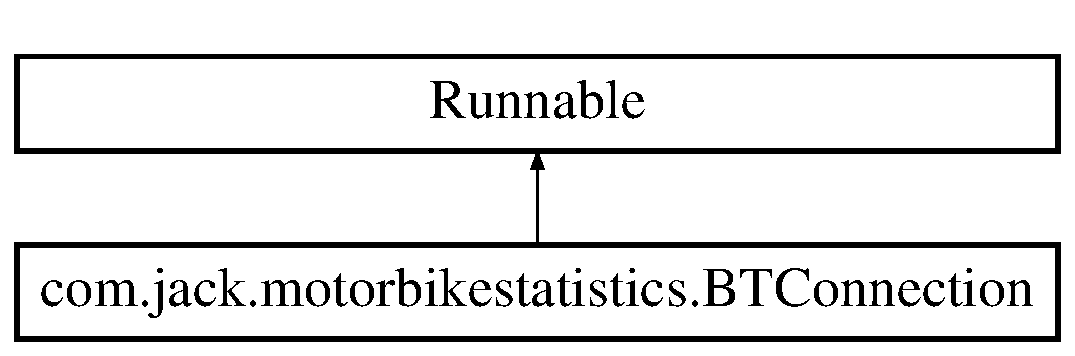
\includegraphics[height=2.000000cm]{classcom_1_1jack_1_1motorbikestatistics_1_1_b_t_connection}
\end{center}
\end{figure}
\subsection*{Public Member Functions}
\begin{DoxyCompactItemize}
\item 
\mbox{\Hypertarget{classcom_1_1jack_1_1motorbikestatistics_1_1_b_t_connection_a55a1c23b7bcf9dc097b10b62ce7828ba}\label{classcom_1_1jack_1_1motorbikestatistics_1_1_b_t_connection_a55a1c23b7bcf9dc097b10b62ce7828ba}} 
{\bfseries B\+T\+Connection} (Bluetooth\+Device bt\+Device)  throws I\+O\+Exception 
\item 
\mbox{\Hypertarget{classcom_1_1jack_1_1motorbikestatistics_1_1_b_t_connection_aae8ee75e78f5beff98572bf3b13a60b8}\label{classcom_1_1jack_1_1motorbikestatistics_1_1_b_t_connection_aae8ee75e78f5beff98572bf3b13a60b8}} 
void {\bfseries set\+R\+X\+Handler} (Handler new\+Handler)
\item 
\mbox{\Hypertarget{classcom_1_1jack_1_1motorbikestatistics_1_1_b_t_connection_ae4c6a0897742c6a7ccfb0b43d0d987da}\label{classcom_1_1jack_1_1motorbikestatistics_1_1_b_t_connection_ae4c6a0897742c6a7ccfb0b43d0d987da}} 
void {\bfseries run} ()
\item 
\mbox{\Hypertarget{classcom_1_1jack_1_1motorbikestatistics_1_1_b_t_connection_a229363b085c81e1a42037075b675677d}\label{classcom_1_1jack_1_1motorbikestatistics_1_1_b_t_connection_a229363b085c81e1a42037075b675677d}} 
void {\bfseries stop} ()
\item 
\mbox{\Hypertarget{classcom_1_1jack_1_1motorbikestatistics_1_1_b_t_connection_a17b07494b0e7cba2e550054d7b47e309}\label{classcom_1_1jack_1_1motorbikestatistics_1_1_b_t_connection_a17b07494b0e7cba2e550054d7b47e309}} 
boolean {\bfseries is\+Running} ()
\item 
\mbox{\Hypertarget{classcom_1_1jack_1_1motorbikestatistics_1_1_b_t_connection_a22f33e46d9f460d78865d4c63b645357}\label{classcom_1_1jack_1_1motorbikestatistics_1_1_b_t_connection_a22f33e46d9f460d78865d4c63b645357}} 
boolean {\bfseries is\+Connected} ()
\end{DoxyCompactItemize}
\subsection*{Public Attributes}
\begin{DoxyCompactItemize}
\item 
final Handler {\bfseries tx\+Handler}
\end{DoxyCompactItemize}


\subsection{Detailed Description}
Created by Jack on 26-\/\+Jan-\/17. 

\subsection{Member Data Documentation}
\mbox{\Hypertarget{classcom_1_1jack_1_1motorbikestatistics_1_1_b_t_connection_a7a88b2007af6a9a5c8667a9f1df980cc}\label{classcom_1_1jack_1_1motorbikestatistics_1_1_b_t_connection_a7a88b2007af6a9a5c8667a9f1df980cc}} 
\index{com\+::jack\+::motorbikestatistics\+::\+B\+T\+Connection@{com\+::jack\+::motorbikestatistics\+::\+B\+T\+Connection}!tx\+Handler@{tx\+Handler}}
\index{tx\+Handler@{tx\+Handler}!com\+::jack\+::motorbikestatistics\+::\+B\+T\+Connection@{com\+::jack\+::motorbikestatistics\+::\+B\+T\+Connection}}
\subsubsection{\texorpdfstring{tx\+Handler}{txHandler}}
{\footnotesize\ttfamily final Handler com.\+jack.\+motorbikestatistics.\+B\+T\+Connection.\+tx\+Handler}

{\bfseries Initial value\+:}
\begin{DoxyCode}
= \textcolor{keyword}{new} Handler(Looper.getMainLooper()) \{

        @Override
        \textcolor{keyword}{public} \textcolor{keywordtype}{void} handleMessage(Message msg) \{

            
            \textcolor{keywordflow}{if} (isConnected() && isRunning()) \{
                OutputStream TXStream;

                
                \textcolor{keywordflow}{try} \{
                    TXStream = btSocket.getOutputStream();

                    String txString = (String)msg.obj;
                    TXStream.write(txString.getBytes());
                \} \textcolor{keywordflow}{catch} (IOException e) \{
                    Log.e(TAG, \textcolor{stringliteral}{"Unable to use TXStream"}, e);
                    \textcolor{keywordflow}{return};
                \}
            \}
        \}
    \}
\end{DoxyCode}


The documentation for this class was generated from the following file\+:\begin{DoxyCompactItemize}
\item 
android-\/app/app/src/main/java/com/jack/motorbikestatistics/B\+T\+Connection.\+java\end{DoxyCompactItemize}

\hypertarget{classcom_1_1jack_1_1motorbikestatistics_1_1_b_t_device_item}{}\section{com.\+jack.\+motorbikestatistics.\+B\+T\+Device\+Item Class Reference}
\label{classcom_1_1jack_1_1motorbikestatistics_1_1_b_t_device_item}\index{com.\+jack.\+motorbikestatistics.\+B\+T\+Device\+Item@{com.\+jack.\+motorbikestatistics.\+B\+T\+Device\+Item}}
\subsection*{Public Member Functions}
\begin{DoxyCompactItemize}
\item 
\hyperlink{classcom_1_1jack_1_1motorbikestatistics_1_1_b_t_connection}{B\+T\+Connection} \hyperlink{classcom_1_1jack_1_1motorbikestatistics_1_1_b_t_device_item_ac3fbff10e5a5b3142ef648bf186b9be0}{get\+Connection} ()
\begin{DoxyCompactList}\small\item\em Getter for the bluetooth connection of specified device. \end{DoxyCompactList}\item 
void \hyperlink{classcom_1_1jack_1_1motorbikestatistics_1_1_b_t_device_item_a96f7261d9eab97d74569fbc3b0da4f28}{set\+Connection} (\hyperlink{classcom_1_1jack_1_1motorbikestatistics_1_1_b_t_connection}{B\+T\+Connection} new\+Conn)
\begin{DoxyCompactList}\small\item\em Setter for setting the Device\+Item object\textquotesingle{}s connection. \end{DoxyCompactList}\item 
Bluetooth\+Device \hyperlink{classcom_1_1jack_1_1motorbikestatistics_1_1_b_t_device_item_aab406fd517db729f7803d48546fd1a95}{get\+Device} ()
\begin{DoxyCompactList}\small\item\em Getter for BT device object (contains name, H\+W\+ID etc.). \end{DoxyCompactList}\item 
String \hyperlink{classcom_1_1jack_1_1motorbikestatistics_1_1_b_t_device_item_aee33189f94c2a428ac67301b536dd004}{get\+Status} ()
\begin{DoxyCompactList}\small\item\em Getter for current status of \hyperlink{classcom_1_1jack_1_1motorbikestatistics_1_1_b_t_device_item}{B\+T\+Device\+Item}. \end{DoxyCompactList}\item 
void \hyperlink{classcom_1_1jack_1_1motorbikestatistics_1_1_b_t_device_item_a4e3d0774e91c5261963b03d6dcb08561}{set\+Status} (String new\+Status)
\begin{DoxyCompactList}\small\item\em Setter for current status of \hyperlink{classcom_1_1jack_1_1motorbikestatistics_1_1_b_t_device_item}{B\+T\+Device\+Item}. \end{DoxyCompactList}\item 
int \hyperlink{classcom_1_1jack_1_1motorbikestatistics_1_1_b_t_device_item_a9e16b980dbddfdb9347ffa6237b78de5}{get\+Icon\+ID} ()
\begin{DoxyCompactList}\small\item\em Getter for icon ID to use in List\+View. \end{DoxyCompactList}\item 
void \hyperlink{classcom_1_1jack_1_1motorbikestatistics_1_1_b_t_device_item_a40eb2a1f46700690d2327bf37bc5ed0e}{set\+Icon\+ID} (int new\+ID)
\begin{DoxyCompactList}\small\item\em Setter for icon ID to use in List\+View. \end{DoxyCompactList}\item 
\hyperlink{classcom_1_1jack_1_1motorbikestatistics_1_1_b_t_device_item_addc508fe41b31b9e13a9105464a627ac}{B\+T\+Device\+Item} (Bluetooth\+Device \hyperlink{classcom_1_1jack_1_1motorbikestatistics_1_1_b_t_device_item_acd943b008d77dcb5d72f8a65fa4986b9}{device}, String \hyperlink{classcom_1_1jack_1_1motorbikestatistics_1_1_b_t_device_item_ae7a8756973644c5719d5faddf3fa7946}{status}, int \hyperlink{classcom_1_1jack_1_1motorbikestatistics_1_1_b_t_device_item_a77f7a3c228f87fa5e946fe77b310f805}{icon\+ID})
\begin{DoxyCompactList}\small\item\em Constructor for \hyperlink{classcom_1_1jack_1_1motorbikestatistics_1_1_b_t_device_item}{B\+T\+Device\+Item} class. \end{DoxyCompactList}\end{DoxyCompactItemize}
\subsection*{Private Attributes}
\begin{DoxyCompactItemize}
\item 
\mbox{\Hypertarget{classcom_1_1jack_1_1motorbikestatistics_1_1_b_t_device_item_a38830528ad49afd7ba09ced7ab55d6dc}\label{classcom_1_1jack_1_1motorbikestatistics_1_1_b_t_device_item_a38830528ad49afd7ba09ced7ab55d6dc}} 
\hyperlink{classcom_1_1jack_1_1motorbikestatistics_1_1_b_t_connection}{B\+T\+Connection} \hyperlink{classcom_1_1jack_1_1motorbikestatistics_1_1_b_t_device_item_a38830528ad49afd7ba09ced7ab55d6dc}{connection} = null
\begin{DoxyCompactList}\small\item\em Variable for \hyperlink{classcom_1_1jack_1_1motorbikestatistics_1_1_b_t_connection}{B\+T\+Connection} if device is already connected. \end{DoxyCompactList}\item 
\mbox{\Hypertarget{classcom_1_1jack_1_1motorbikestatistics_1_1_b_t_device_item_a77f7a3c228f87fa5e946fe77b310f805}\label{classcom_1_1jack_1_1motorbikestatistics_1_1_b_t_device_item_a77f7a3c228f87fa5e946fe77b310f805}} 
int \hyperlink{classcom_1_1jack_1_1motorbikestatistics_1_1_b_t_device_item_a77f7a3c228f87fa5e946fe77b310f805}{icon\+ID}
\begin{DoxyCompactList}\small\item\em ID of icon to use within the List\+View. \end{DoxyCompactList}\item 
\mbox{\Hypertarget{classcom_1_1jack_1_1motorbikestatistics_1_1_b_t_device_item_acd943b008d77dcb5d72f8a65fa4986b9}\label{classcom_1_1jack_1_1motorbikestatistics_1_1_b_t_device_item_acd943b008d77dcb5d72f8a65fa4986b9}} 
Bluetooth\+Device \hyperlink{classcom_1_1jack_1_1motorbikestatistics_1_1_b_t_device_item_acd943b008d77dcb5d72f8a65fa4986b9}{device}
\begin{DoxyCompactList}\small\item\em Device object that holds info such as name, H\+W\+ID etc. \end{DoxyCompactList}\item 
\mbox{\Hypertarget{classcom_1_1jack_1_1motorbikestatistics_1_1_b_t_device_item_ae7a8756973644c5719d5faddf3fa7946}\label{classcom_1_1jack_1_1motorbikestatistics_1_1_b_t_device_item_ae7a8756973644c5719d5faddf3fa7946}} 
String \hyperlink{classcom_1_1jack_1_1motorbikestatistics_1_1_b_t_device_item_ae7a8756973644c5719d5faddf3fa7946}{status}
\begin{DoxyCompactList}\small\item\em Status of the device, unpaired, paired, connected. \end{DoxyCompactList}\end{DoxyCompactItemize}


\subsection{Constructor \& Destructor Documentation}
\mbox{\Hypertarget{classcom_1_1jack_1_1motorbikestatistics_1_1_b_t_device_item_addc508fe41b31b9e13a9105464a627ac}\label{classcom_1_1jack_1_1motorbikestatistics_1_1_b_t_device_item_addc508fe41b31b9e13a9105464a627ac}} 
\index{com\+::jack\+::motorbikestatistics\+::\+B\+T\+Device\+Item@{com\+::jack\+::motorbikestatistics\+::\+B\+T\+Device\+Item}!B\+T\+Device\+Item@{B\+T\+Device\+Item}}
\index{B\+T\+Device\+Item@{B\+T\+Device\+Item}!com\+::jack\+::motorbikestatistics\+::\+B\+T\+Device\+Item@{com\+::jack\+::motorbikestatistics\+::\+B\+T\+Device\+Item}}
\subsubsection{\texorpdfstring{B\+T\+Device\+Item()}{BTDeviceItem()}}
{\footnotesize\ttfamily com.\+jack.\+motorbikestatistics.\+B\+T\+Device\+Item.\+B\+T\+Device\+Item (\begin{DoxyParamCaption}\item[{Bluetooth\+Device}]{device,  }\item[{String}]{status,  }\item[{int}]{icon\+ID }\end{DoxyParamCaption})\hspace{0.3cm}{\ttfamily [inline]}}



Constructor for \hyperlink{classcom_1_1jack_1_1motorbikestatistics_1_1_b_t_device_item}{B\+T\+Device\+Item} class. 

Called when new Bluetooth\+Device is found during discovery, so that it can be added to the device List\+View.


\begin{DoxyParams}{Parameters}
{\em device} & -\/ Bluetooth\+Device containing H\+W\+ID, name, etc. \\
\hline
{\em status} & -\/ Current status of the discovered device. \\
\hline
{\em icon\+ID} & -\/ Icon ID to display within the List\+View. \\
\hline
\end{DoxyParams}


References com.\+jack.\+motorbikestatistics.\+B\+T\+Device\+Item.\+device, com.\+jack.\+motorbikestatistics.\+B\+T\+Device\+Item.\+icon\+ID, and com.\+jack.\+motorbikestatistics.\+B\+T\+Device\+Item.\+status.


\begin{DoxyCode}
93     \{
94         this.\hyperlink{classcom_1_1jack_1_1motorbikestatistics_1_1_b_t_device_item_acd943b008d77dcb5d72f8a65fa4986b9}{device} = \hyperlink{classcom_1_1jack_1_1motorbikestatistics_1_1_b_t_device_item_acd943b008d77dcb5d72f8a65fa4986b9}{device};
95         this.\hyperlink{classcom_1_1jack_1_1motorbikestatistics_1_1_b_t_device_item_ae7a8756973644c5719d5faddf3fa7946}{status} = \hyperlink{classcom_1_1jack_1_1motorbikestatistics_1_1_b_t_device_item_ae7a8756973644c5719d5faddf3fa7946}{status};
96         this.\hyperlink{classcom_1_1jack_1_1motorbikestatistics_1_1_b_t_device_item_a77f7a3c228f87fa5e946fe77b310f805}{iconID} = \hyperlink{classcom_1_1jack_1_1motorbikestatistics_1_1_b_t_device_item_a77f7a3c228f87fa5e946fe77b310f805}{iconID};
97     \}
\end{DoxyCode}


\subsection{Member Function Documentation}
\mbox{\Hypertarget{classcom_1_1jack_1_1motorbikestatistics_1_1_b_t_device_item_ac3fbff10e5a5b3142ef648bf186b9be0}\label{classcom_1_1jack_1_1motorbikestatistics_1_1_b_t_device_item_ac3fbff10e5a5b3142ef648bf186b9be0}} 
\index{com\+::jack\+::motorbikestatistics\+::\+B\+T\+Device\+Item@{com\+::jack\+::motorbikestatistics\+::\+B\+T\+Device\+Item}!get\+Connection@{get\+Connection}}
\index{get\+Connection@{get\+Connection}!com\+::jack\+::motorbikestatistics\+::\+B\+T\+Device\+Item@{com\+::jack\+::motorbikestatistics\+::\+B\+T\+Device\+Item}}
\subsubsection{\texorpdfstring{get\+Connection()}{getConnection()}}
{\footnotesize\ttfamily \hyperlink{classcom_1_1jack_1_1motorbikestatistics_1_1_b_t_connection}{B\+T\+Connection} com.\+jack.\+motorbikestatistics.\+B\+T\+Device\+Item.\+get\+Connection (\begin{DoxyParamCaption}{ }\end{DoxyParamCaption})\hspace{0.3cm}{\ttfamily [inline]}}



Getter for the bluetooth connection of specified device. 

\begin{DoxyReturn}{Returns}
\hyperlink{classcom_1_1jack_1_1motorbikestatistics_1_1_b_t_connection}{B\+T\+Connection} -\/ Connection between app \& logging device. 
\end{DoxyReturn}


References com.\+jack.\+motorbikestatistics.\+B\+T\+Device\+Item.\+connection.


\begin{DoxyCode}
30                                         \{
31         \textcolor{keywordflow}{return} \hyperlink{classcom_1_1jack_1_1motorbikestatistics_1_1_b_t_device_item_a38830528ad49afd7ba09ced7ab55d6dc}{connection};
32     \}
\end{DoxyCode}
\mbox{\Hypertarget{classcom_1_1jack_1_1motorbikestatistics_1_1_b_t_device_item_a96f7261d9eab97d74569fbc3b0da4f28}\label{classcom_1_1jack_1_1motorbikestatistics_1_1_b_t_device_item_a96f7261d9eab97d74569fbc3b0da4f28}} 
\index{com\+::jack\+::motorbikestatistics\+::\+B\+T\+Device\+Item@{com\+::jack\+::motorbikestatistics\+::\+B\+T\+Device\+Item}!set\+Connection@{set\+Connection}}
\index{set\+Connection@{set\+Connection}!com\+::jack\+::motorbikestatistics\+::\+B\+T\+Device\+Item@{com\+::jack\+::motorbikestatistics\+::\+B\+T\+Device\+Item}}
\subsubsection{\texorpdfstring{set\+Connection()}{setConnection()}}
{\footnotesize\ttfamily void com.\+jack.\+motorbikestatistics.\+B\+T\+Device\+Item.\+set\+Connection (\begin{DoxyParamCaption}\item[{\hyperlink{classcom_1_1jack_1_1motorbikestatistics_1_1_b_t_connection}{B\+T\+Connection}}]{new\+Conn }\end{DoxyParamCaption})\hspace{0.3cm}{\ttfamily [inline]}}



Setter for setting the Device\+Item object\textquotesingle{}s connection. 


\begin{DoxyParams}{Parameters}
{\em new\+Conn} & -\/ New connection between app \& logging device. \\
\hline
\end{DoxyParams}

\begin{DoxyCode}
38                                                     \{
39         \hyperlink{classcom_1_1jack_1_1motorbikestatistics_1_1_b_t_device_item_a38830528ad49afd7ba09ced7ab55d6dc}{connection} = newConn;
40     \}
\end{DoxyCode}
\mbox{\Hypertarget{classcom_1_1jack_1_1motorbikestatistics_1_1_b_t_device_item_aab406fd517db729f7803d48546fd1a95}\label{classcom_1_1jack_1_1motorbikestatistics_1_1_b_t_device_item_aab406fd517db729f7803d48546fd1a95}} 
\index{com\+::jack\+::motorbikestatistics\+::\+B\+T\+Device\+Item@{com\+::jack\+::motorbikestatistics\+::\+B\+T\+Device\+Item}!get\+Device@{get\+Device}}
\index{get\+Device@{get\+Device}!com\+::jack\+::motorbikestatistics\+::\+B\+T\+Device\+Item@{com\+::jack\+::motorbikestatistics\+::\+B\+T\+Device\+Item}}
\subsubsection{\texorpdfstring{get\+Device()}{getDevice()}}
{\footnotesize\ttfamily Bluetooth\+Device com.\+jack.\+motorbikestatistics.\+B\+T\+Device\+Item.\+get\+Device (\begin{DoxyParamCaption}{ }\end{DoxyParamCaption})\hspace{0.3cm}{\ttfamily [inline]}}



Getter for BT device object (contains name, H\+W\+ID etc.). 

\begin{DoxyReturn}{Returns}
Bluetooth\+Device -\/ The bluetooth device object. 
\end{DoxyReturn}


References com.\+jack.\+motorbikestatistics.\+B\+T\+Device\+Item.\+device.


\begin{DoxyCode}
46                                        \{
47         \textcolor{keywordflow}{return} \hyperlink{classcom_1_1jack_1_1motorbikestatistics_1_1_b_t_device_item_acd943b008d77dcb5d72f8a65fa4986b9}{device};
48     \}
\end{DoxyCode}
\mbox{\Hypertarget{classcom_1_1jack_1_1motorbikestatistics_1_1_b_t_device_item_aee33189f94c2a428ac67301b536dd004}\label{classcom_1_1jack_1_1motorbikestatistics_1_1_b_t_device_item_aee33189f94c2a428ac67301b536dd004}} 
\index{com\+::jack\+::motorbikestatistics\+::\+B\+T\+Device\+Item@{com\+::jack\+::motorbikestatistics\+::\+B\+T\+Device\+Item}!get\+Status@{get\+Status}}
\index{get\+Status@{get\+Status}!com\+::jack\+::motorbikestatistics\+::\+B\+T\+Device\+Item@{com\+::jack\+::motorbikestatistics\+::\+B\+T\+Device\+Item}}
\subsubsection{\texorpdfstring{get\+Status()}{getStatus()}}
{\footnotesize\ttfamily String com.\+jack.\+motorbikestatistics.\+B\+T\+Device\+Item.\+get\+Status (\begin{DoxyParamCaption}{ }\end{DoxyParamCaption})\hspace{0.3cm}{\ttfamily [inline]}}



Getter for current status of \hyperlink{classcom_1_1jack_1_1motorbikestatistics_1_1_b_t_device_item}{B\+T\+Device\+Item}. 

\begin{DoxyReturn}{Returns}
String -\/ Current status\+: unpaired, paired or connected. 
\end{DoxyReturn}


References com.\+jack.\+motorbikestatistics.\+B\+T\+Device\+Item.\+status.


\begin{DoxyCode}
54                               \{
55         \textcolor{keywordflow}{return} \hyperlink{classcom_1_1jack_1_1motorbikestatistics_1_1_b_t_device_item_ae7a8756973644c5719d5faddf3fa7946}{status};
56     \}
\end{DoxyCode}
\mbox{\Hypertarget{classcom_1_1jack_1_1motorbikestatistics_1_1_b_t_device_item_a4e3d0774e91c5261963b03d6dcb08561}\label{classcom_1_1jack_1_1motorbikestatistics_1_1_b_t_device_item_a4e3d0774e91c5261963b03d6dcb08561}} 
\index{com\+::jack\+::motorbikestatistics\+::\+B\+T\+Device\+Item@{com\+::jack\+::motorbikestatistics\+::\+B\+T\+Device\+Item}!set\+Status@{set\+Status}}
\index{set\+Status@{set\+Status}!com\+::jack\+::motorbikestatistics\+::\+B\+T\+Device\+Item@{com\+::jack\+::motorbikestatistics\+::\+B\+T\+Device\+Item}}
\subsubsection{\texorpdfstring{set\+Status()}{setStatus()}}
{\footnotesize\ttfamily void com.\+jack.\+motorbikestatistics.\+B\+T\+Device\+Item.\+set\+Status (\begin{DoxyParamCaption}\item[{String}]{new\+Status }\end{DoxyParamCaption})\hspace{0.3cm}{\ttfamily [inline]}}



Setter for current status of \hyperlink{classcom_1_1jack_1_1motorbikestatistics_1_1_b_t_device_item}{B\+T\+Device\+Item}. 


\begin{DoxyParams}{Parameters}
{\em new\+Status} & -\/ New string for status. \\
\hline
\end{DoxyParams}

\begin{DoxyCode}
62                                             \{
63         \hyperlink{classcom_1_1jack_1_1motorbikestatistics_1_1_b_t_device_item_ae7a8756973644c5719d5faddf3fa7946}{status} = newStatus;
64     \}
\end{DoxyCode}
\mbox{\Hypertarget{classcom_1_1jack_1_1motorbikestatistics_1_1_b_t_device_item_a9e16b980dbddfdb9347ffa6237b78de5}\label{classcom_1_1jack_1_1motorbikestatistics_1_1_b_t_device_item_a9e16b980dbddfdb9347ffa6237b78de5}} 
\index{com\+::jack\+::motorbikestatistics\+::\+B\+T\+Device\+Item@{com\+::jack\+::motorbikestatistics\+::\+B\+T\+Device\+Item}!get\+Icon\+ID@{get\+Icon\+ID}}
\index{get\+Icon\+ID@{get\+Icon\+ID}!com\+::jack\+::motorbikestatistics\+::\+B\+T\+Device\+Item@{com\+::jack\+::motorbikestatistics\+::\+B\+T\+Device\+Item}}
\subsubsection{\texorpdfstring{get\+Icon\+I\+D()}{getIconID()}}
{\footnotesize\ttfamily int com.\+jack.\+motorbikestatistics.\+B\+T\+Device\+Item.\+get\+Icon\+ID (\begin{DoxyParamCaption}{ }\end{DoxyParamCaption})\hspace{0.3cm}{\ttfamily [inline]}}



Getter for icon ID to use in List\+View. 

\begin{DoxyReturn}{Returns}
int -\/ Icon ID to use. 
\end{DoxyReturn}


References com.\+jack.\+motorbikestatistics.\+B\+T\+Device\+Item.\+icon\+ID.


\begin{DoxyCode}
70                            \{
71         \textcolor{keywordflow}{return} \hyperlink{classcom_1_1jack_1_1motorbikestatistics_1_1_b_t_device_item_a77f7a3c228f87fa5e946fe77b310f805}{iconID};
72     \}
\end{DoxyCode}
\mbox{\Hypertarget{classcom_1_1jack_1_1motorbikestatistics_1_1_b_t_device_item_a40eb2a1f46700690d2327bf37bc5ed0e}\label{classcom_1_1jack_1_1motorbikestatistics_1_1_b_t_device_item_a40eb2a1f46700690d2327bf37bc5ed0e}} 
\index{com\+::jack\+::motorbikestatistics\+::\+B\+T\+Device\+Item@{com\+::jack\+::motorbikestatistics\+::\+B\+T\+Device\+Item}!set\+Icon\+ID@{set\+Icon\+ID}}
\index{set\+Icon\+ID@{set\+Icon\+ID}!com\+::jack\+::motorbikestatistics\+::\+B\+T\+Device\+Item@{com\+::jack\+::motorbikestatistics\+::\+B\+T\+Device\+Item}}
\subsubsection{\texorpdfstring{set\+Icon\+I\+D()}{setIconID()}}
{\footnotesize\ttfamily void com.\+jack.\+motorbikestatistics.\+B\+T\+Device\+Item.\+set\+Icon\+ID (\begin{DoxyParamCaption}\item[{int}]{new\+ID }\end{DoxyParamCaption})\hspace{0.3cm}{\ttfamily [inline]}}



Setter for icon ID to use in List\+View. 


\begin{DoxyParams}{Parameters}
{\em new\+ID} & -\/ New icon ID to use. \\
\hline
\end{DoxyParams}

\begin{DoxyCode}
78                                      \{
79         \hyperlink{classcom_1_1jack_1_1motorbikestatistics_1_1_b_t_device_item_a77f7a3c228f87fa5e946fe77b310f805}{iconID} = newID;
80     \}
\end{DoxyCode}


The documentation for this class was generated from the following file\+:\begin{DoxyCompactItemize}
\item 
android-\/app/app/src/main/java/com/jack/motorbikestatistics/\hyperlink{_b_t_device_item_8java}{B\+T\+Device\+Item.\+java}\end{DoxyCompactItemize}

\hypertarget{classcom_1_1jack_1_1motorbikestatistics_1_1_b_t_device_list_adapter}{}\section{com.\+jack.\+motorbikestatistics.\+B\+T\+Device\+List\+Adapter Class Reference}
\label{classcom_1_1jack_1_1motorbikestatistics_1_1_b_t_device_list_adapter}\index{com.\+jack.\+motorbikestatistics.\+B\+T\+Device\+List\+Adapter@{com.\+jack.\+motorbikestatistics.\+B\+T\+Device\+List\+Adapter}}
Inheritance diagram for com.\+jack.\+motorbikestatistics.\+B\+T\+Device\+List\+Adapter\+:\begin{figure}[H]
\begin{center}
\leavevmode
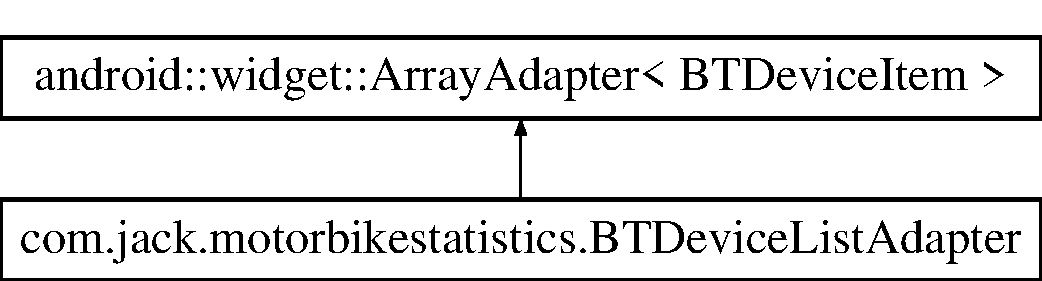
\includegraphics[height=2.000000cm]{classcom_1_1jack_1_1motorbikestatistics_1_1_b_t_device_list_adapter}
\end{center}
\end{figure}
\subsection*{Public Member Functions}
\begin{DoxyCompactItemize}
\item 
\mbox{\Hypertarget{classcom_1_1jack_1_1motorbikestatistics_1_1_b_t_device_list_adapter_a103bf9deb20f6a547537da994f66b92f}\label{classcom_1_1jack_1_1motorbikestatistics_1_1_b_t_device_list_adapter_a103bf9deb20f6a547537da994f66b92f}} 
{\bfseries B\+T\+Device\+List\+Adapter} (Context cnt, int layout\+Resource\+Id, Array\+List$<$ \hyperlink{classcom_1_1jack_1_1motorbikestatistics_1_1_b_t_device_item}{B\+T\+Device\+Item} $>$ data, Bluetooth\+Adapter adapter)
\item 
\mbox{\Hypertarget{classcom_1_1jack_1_1motorbikestatistics_1_1_b_t_device_list_adapter_ab9e3230f609c8a8195c3e4e9c2b26b2e}\label{classcom_1_1jack_1_1motorbikestatistics_1_1_b_t_device_list_adapter_ab9e3230f609c8a8195c3e4e9c2b26b2e}} 
View {\bfseries get\+View} (int position, View convert\+View, View\+Group parent)
\end{DoxyCompactItemize}


\subsection{Detailed Description}
Created by Jack on 25-\/\+Jan-\/17. 

The documentation for this class was generated from the following file\+:\begin{DoxyCompactItemize}
\item 
android-\/app/app/src/main/java/com/jack/motorbikestatistics/B\+T\+Device\+List\+Adapter.\+java\end{DoxyCompactItemize}

\hypertarget{classcom_1_1jack_1_1motorbikestatistics_1_1_data_item}{}\section{com.\+jack.\+motorbikestatistics.\+Data\+Item$<$ T $>$ Class Template Reference}
\label{classcom_1_1jack_1_1motorbikestatistics_1_1_data_item}\index{com.\+jack.\+motorbikestatistics.\+Data\+Item$<$ T $>$@{com.\+jack.\+motorbikestatistics.\+Data\+Item$<$ T $>$}}
\subsection*{Public Member Functions}
\begin{DoxyCompactItemize}
\item 
\mbox{\Hypertarget{classcom_1_1jack_1_1motorbikestatistics_1_1_data_item_ae7367bc22bb0d8dc831944c7ce4f39f9}\label{classcom_1_1jack_1_1motorbikestatistics_1_1_data_item_ae7367bc22bb0d8dc831944c7ce4f39f9}} 
{\bfseries Data\+Item} (String name, boolean avg\+Min\+Max)
\item 
\mbox{\Hypertarget{classcom_1_1jack_1_1motorbikestatistics_1_1_data_item_a5bb494fbf02f8157b859694d3c2671d6}\label{classcom_1_1jack_1_1motorbikestatistics_1_1_data_item_a5bb494fbf02f8157b859694d3c2671d6}} 
{\bfseries Data\+Item} (String name, boolean avg\+Min\+Max, T value)
\item 
\mbox{\Hypertarget{classcom_1_1jack_1_1motorbikestatistics_1_1_data_item_ae0beb1548c3ca85be62eb2e94e9def65}\label{classcom_1_1jack_1_1motorbikestatistics_1_1_data_item_ae0beb1548c3ca85be62eb2e94e9def65}} 
String {\bfseries get\+Name} ()
\item 
\mbox{\Hypertarget{classcom_1_1jack_1_1motorbikestatistics_1_1_data_item_af9fd13d6997dbf73dfacaaa33f6f3d9e}\label{classcom_1_1jack_1_1motorbikestatistics_1_1_data_item_af9fd13d6997dbf73dfacaaa33f6f3d9e}} 
boolean {\bfseries get\+Enabled\+Avg\+Min\+Max} ()
\item 
\mbox{\Hypertarget{classcom_1_1jack_1_1motorbikestatistics_1_1_data_item_aad19eefe19453103b36ceabca8b1154c}\label{classcom_1_1jack_1_1motorbikestatistics_1_1_data_item_aad19eefe19453103b36ceabca8b1154c}} 
T {\bfseries get\+Current} ()
\item 
\mbox{\Hypertarget{classcom_1_1jack_1_1motorbikestatistics_1_1_data_item_af8e5083ad7651708f7def6b488e881d2}\label{classcom_1_1jack_1_1motorbikestatistics_1_1_data_item_af8e5083ad7651708f7def6b488e881d2}} 
Double {\bfseries get\+Average} ()
\item 
\mbox{\Hypertarget{classcom_1_1jack_1_1motorbikestatistics_1_1_data_item_a45cdf3ef773c9c1e69d12861deaccec0}\label{classcom_1_1jack_1_1motorbikestatistics_1_1_data_item_a45cdf3ef773c9c1e69d12861deaccec0}} 
T {\bfseries get\+Minimum} ()
\item 
\mbox{\Hypertarget{classcom_1_1jack_1_1motorbikestatistics_1_1_data_item_a5d58df64d90e56c7bb7e8aa8bf49aa0f}\label{classcom_1_1jack_1_1motorbikestatistics_1_1_data_item_a5d58df64d90e56c7bb7e8aa8bf49aa0f}} 
T {\bfseries get\+Maximum} ()
\item 
\mbox{\Hypertarget{classcom_1_1jack_1_1motorbikestatistics_1_1_data_item_abdeab9f088a2a78f66ac852993b555ca}\label{classcom_1_1jack_1_1motorbikestatistics_1_1_data_item_abdeab9f088a2a78f66ac852993b555ca}} 
void {\bfseries set\+Current} (T value)
\end{DoxyCompactItemize}


\subsection{Detailed Description}
Created by Jack on 05-\/\+Mar-\/17. 

The documentation for this class was generated from the following file\+:\begin{DoxyCompactItemize}
\item 
android-\/app/app/src/main/java/com/jack/motorbikestatistics/Data\+Item.\+java\end{DoxyCompactItemize}

\hypertarget{classcom_1_1jack_1_1motorbikestatistics_1_1_data_list_adapter}{}\section{com.\+jack.\+motorbikestatistics.\+Data\+List\+Adapter Class Reference}
\label{classcom_1_1jack_1_1motorbikestatistics_1_1_data_list_adapter}\index{com.\+jack.\+motorbikestatistics.\+Data\+List\+Adapter@{com.\+jack.\+motorbikestatistics.\+Data\+List\+Adapter}}
Inheritance diagram for com.\+jack.\+motorbikestatistics.\+Data\+List\+Adapter\+:\begin{figure}[H]
\begin{center}
\leavevmode
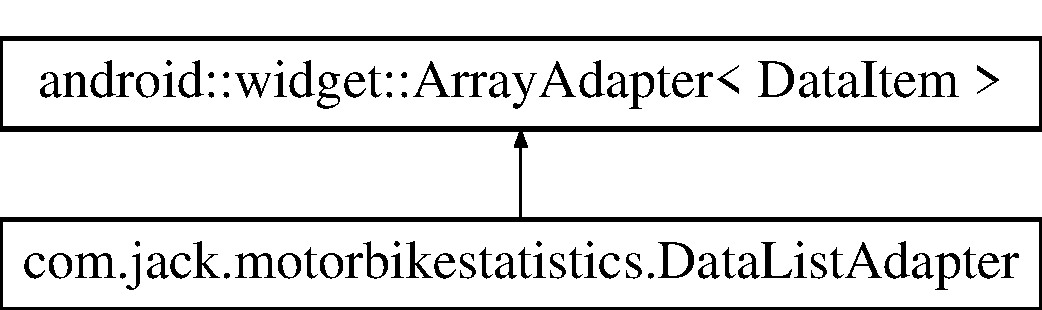
\includegraphics[height=2.000000cm]{classcom_1_1jack_1_1motorbikestatistics_1_1_data_list_adapter}
\end{center}
\end{figure}
\subsection*{Public Member Functions}
\begin{DoxyCompactItemize}
\item 
\mbox{\Hypertarget{classcom_1_1jack_1_1motorbikestatistics_1_1_data_list_adapter_aa9aad25299a2df8a357569b6eb3c28b5}\label{classcom_1_1jack_1_1motorbikestatistics_1_1_data_list_adapter_aa9aad25299a2df8a357569b6eb3c28b5}} 
{\bfseries Data\+List\+Adapter} (Context cnt, int layout\+Resource\+Id, Array\+List$<$ \hyperlink{classcom_1_1jack_1_1motorbikestatistics_1_1_data_item}{Data\+Item} $>$ data)
\item 
\mbox{\Hypertarget{classcom_1_1jack_1_1motorbikestatistics_1_1_data_list_adapter_a724cb5f4a43bba97dbfdbc08aa9e3015}\label{classcom_1_1jack_1_1motorbikestatistics_1_1_data_list_adapter_a724cb5f4a43bba97dbfdbc08aa9e3015}} 
View {\bfseries get\+View} (int position, View convert\+View, View\+Group parent)
\end{DoxyCompactItemize}


\subsection{Detailed Description}
Created by Jack on 05-\/\+Mar-\/17. 

The documentation for this class was generated from the following file\+:\begin{DoxyCompactItemize}
\item 
android-\/app/app/src/main/java/com/jack/motorbikestatistics/Data\+List\+Adapter.\+java\end{DoxyCompactItemize}

\hypertarget{classcom_1_1jack_1_1motorbikestatistics_1_1_load_device_fragment}{}\section{com.\+jack.\+motorbikestatistics.\+Load\+Device\+Fragment Class Reference}
\label{classcom_1_1jack_1_1motorbikestatistics_1_1_load_device_fragment}\index{com.\+jack.\+motorbikestatistics.\+Load\+Device\+Fragment@{com.\+jack.\+motorbikestatistics.\+Load\+Device\+Fragment}}
Inheritance diagram for com.\+jack.\+motorbikestatistics.\+Load\+Device\+Fragment\+:\begin{figure}[H]
\begin{center}
\leavevmode
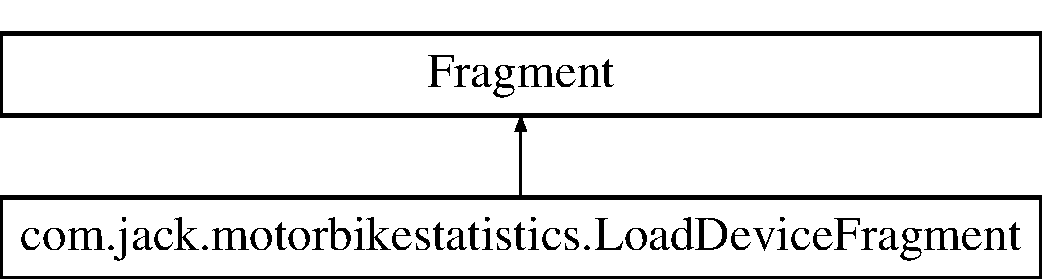
\includegraphics[height=2.000000cm]{classcom_1_1jack_1_1motorbikestatistics_1_1_load_device_fragment}
\end{center}
\end{figure}
\subsection*{Public Member Functions}
\begin{DoxyCompactItemize}
\item 
\mbox{\Hypertarget{classcom_1_1jack_1_1motorbikestatistics_1_1_load_device_fragment_a9ad9f0d9ef69417e2131613009c02338}\label{classcom_1_1jack_1_1motorbikestatistics_1_1_load_device_fragment_a9ad9f0d9ef69417e2131613009c02338}} 
View {\bfseries on\+Create\+View} (Layout\+Inflater inflater, View\+Group container, Bundle saved\+Instance\+State)
\item 
\mbox{\Hypertarget{classcom_1_1jack_1_1motorbikestatistics_1_1_load_device_fragment_aec66dc5fd944098de78ace4175fca5b6}\label{classcom_1_1jack_1_1motorbikestatistics_1_1_load_device_fragment_aec66dc5fd944098de78ace4175fca5b6}} 
void {\bfseries set\+B\+T\+Connection} (\hyperlink{classcom_1_1jack_1_1motorbikestatistics_1_1_b_t_connection}{B\+T\+Connection} bt\+Connection)
\end{DoxyCompactItemize}
\subsection*{Public Attributes}
\begin{DoxyCompactItemize}
\item 
final Handler {\bfseries R\+X\+Handler}
\item 
final List\+View.\+On\+Item\+Click\+Listener {\bfseries trip\+Click\+Listener}
\end{DoxyCompactItemize}
\subsection*{Private Member Functions}
\begin{DoxyCompactItemize}
\item 
\mbox{\Hypertarget{classcom_1_1jack_1_1motorbikestatistics_1_1_load_device_fragment_a23957dbe1518052c7167d86938a14c35}\label{classcom_1_1jack_1_1motorbikestatistics_1_1_load_device_fragment_a23957dbe1518052c7167d86938a14c35}} 
final void {\bfseries add\+Trip} (J\+S\+O\+N\+Object json\+Data)
\end{DoxyCompactItemize}
\subsection*{Private Attributes}
\begin{DoxyCompactItemize}
\item 
\mbox{\Hypertarget{classcom_1_1jack_1_1motorbikestatistics_1_1_load_device_fragment_a7a446c4528638e9d169481c3ff1471b0}\label{classcom_1_1jack_1_1motorbikestatistics_1_1_load_device_fragment_a7a446c4528638e9d169481c3ff1471b0}} 
\hyperlink{classcom_1_1jack_1_1motorbikestatistics_1_1_b_t_connection}{B\+T\+Connection} {\bfseries bt\+Connection} = null
\item 
\mbox{\Hypertarget{classcom_1_1jack_1_1motorbikestatistics_1_1_load_device_fragment_a92be11df86dfe159ecbdaff59e526464}\label{classcom_1_1jack_1_1motorbikestatistics_1_1_load_device_fragment_a92be11df86dfe159ecbdaff59e526464}} 
Array\+List$<$ \hyperlink{classcom_1_1jack_1_1motorbikestatistics_1_1_trip_item}{Trip\+Item} $>$ {\bfseries trip\+List}
\item 
\mbox{\Hypertarget{classcom_1_1jack_1_1motorbikestatistics_1_1_load_device_fragment_a3ccc43db37a3b6d9a7dc345e9ab78d6b}\label{classcom_1_1jack_1_1motorbikestatistics_1_1_load_device_fragment_a3ccc43db37a3b6d9a7dc345e9ab78d6b}} 
Array\+Adapter$<$ \hyperlink{classcom_1_1jack_1_1motorbikestatistics_1_1_trip_item}{Trip\+Item} $>$ {\bfseries lv\+Adapter}
\end{DoxyCompactItemize}
\subsection*{Static Private Attributes}
\begin{DoxyCompactItemize}
\item 
\mbox{\Hypertarget{classcom_1_1jack_1_1motorbikestatistics_1_1_load_device_fragment_aca212e892559df75e77d2d24870195e1}\label{classcom_1_1jack_1_1motorbikestatistics_1_1_load_device_fragment_aca212e892559df75e77d2d24870195e1}} 
static final String {\bfseries N\+E\+W\+\_\+\+L\+I\+NE} = \char`\"{}\textbackslash{}r\textbackslash{}n\char`\"{}
\item 
\mbox{\Hypertarget{classcom_1_1jack_1_1motorbikestatistics_1_1_load_device_fragment_a484328e2963103665fae8801557bef73}\label{classcom_1_1jack_1_1motorbikestatistics_1_1_load_device_fragment_a484328e2963103665fae8801557bef73}} 
static final String {\bfseries L\+O\+A\+D\+\_\+\+T\+R\+I\+P\+\_\+\+C\+H\+AR} = \char`\"{}3\char`\"{}
\end{DoxyCompactItemize}


\subsection{Detailed Description}
Created by Jack on 23-\/\+Jan-\/17. 

\subsection{Member Data Documentation}
\mbox{\Hypertarget{classcom_1_1jack_1_1motorbikestatistics_1_1_load_device_fragment_a7c26c8686c290d8766b051f31473d716}\label{classcom_1_1jack_1_1motorbikestatistics_1_1_load_device_fragment_a7c26c8686c290d8766b051f31473d716}} 
\index{com\+::jack\+::motorbikestatistics\+::\+Load\+Device\+Fragment@{com\+::jack\+::motorbikestatistics\+::\+Load\+Device\+Fragment}!R\+X\+Handler@{R\+X\+Handler}}
\index{R\+X\+Handler@{R\+X\+Handler}!com\+::jack\+::motorbikestatistics\+::\+Load\+Device\+Fragment@{com\+::jack\+::motorbikestatistics\+::\+Load\+Device\+Fragment}}
\subsubsection{\texorpdfstring{R\+X\+Handler}{RXHandler}}
{\footnotesize\ttfamily final Handler com.\+jack.\+motorbikestatistics.\+Load\+Device\+Fragment.\+R\+X\+Handler}

{\bfseries Initial value\+:}
\begin{DoxyCode}
= \textcolor{keyword}{new} Handler(Looper.getMainLooper()) \{

        @Override
        \textcolor{keyword}{public} \textcolor{keywordtype}{void} handleMessage(Message msg) \{

            Bundle msgData = msg.getData();
            String jsonString = msgData.getString(\textcolor{stringliteral}{"JSON"});

            \textcolor{keywordflow}{if} (jsonString != null) \{

                
                \textcolor{keywordflow}{try} \{
                    JSONObject tmpJSON = \textcolor{keyword}{new} JSONObject(jsonString);
                    addTrip(tmpJSON);

                \} \textcolor{keywordflow}{catch} (JSONException e) \{
                    
                \}
            \}
        \}
    \}
\end{DoxyCode}
\mbox{\Hypertarget{classcom_1_1jack_1_1motorbikestatistics_1_1_load_device_fragment_a06ac1ecf82b1709e25421b1b77eb768c}\label{classcom_1_1jack_1_1motorbikestatistics_1_1_load_device_fragment_a06ac1ecf82b1709e25421b1b77eb768c}} 
\index{com\+::jack\+::motorbikestatistics\+::\+Load\+Device\+Fragment@{com\+::jack\+::motorbikestatistics\+::\+Load\+Device\+Fragment}!trip\+Click\+Listener@{trip\+Click\+Listener}}
\index{trip\+Click\+Listener@{trip\+Click\+Listener}!com\+::jack\+::motorbikestatistics\+::\+Load\+Device\+Fragment@{com\+::jack\+::motorbikestatistics\+::\+Load\+Device\+Fragment}}
\subsubsection{\texorpdfstring{trip\+Click\+Listener}{tripClickListener}}
{\footnotesize\ttfamily final List\+View.\+On\+Item\+Click\+Listener com.\+jack.\+motorbikestatistics.\+Load\+Device\+Fragment.\+trip\+Click\+Listener}

{\bfseries Initial value\+:}
\begin{DoxyCode}
= \textcolor{keyword}{new} ListView.OnItemClickListener() \{
        @Override
        \textcolor{keyword}{public} \textcolor{keywordtype}{void} onItemClick(AdapterView<?> parent, View view, \textcolor{keywordtype}{int} position, \textcolor{keywordtype}{long} \textcolor{keywordtype}{id}) \{

            \textcolor{keywordflow}{if} (btConnection != null && btConnection.isConnected()) \{
                TripItem tripItem = (TripItem) parent.getItemAtPosition(position);

                
                RealtimeFragment statFragment = \textcolor{keyword}{new} RealtimeFragment();
                btConnection.setRXHandler(statFragment.RXHandler);

                
                Message message = \textcolor{keyword}{new} Message();
                message.obj = (String) LOAD\_TRIP\_CHAR + tripItem.getTripName();
                message.setTarget(btConnection.txHandler);
                message.sendToTarget();

                FragmentManager fragmentManager = getFragmentManager();
                fragmentManager.beginTransaction()
                        .replace(R.id.content\_frame, statFragment)
                        .commit();
            \}
        \}
    \}
\end{DoxyCode}


The documentation for this class was generated from the following file\+:\begin{DoxyCompactItemize}
\item 
android-\/app/app/src/main/java/com/jack/motorbikestatistics/Load\+Device\+Fragment.\+java\end{DoxyCompactItemize}

\hypertarget{classcom_1_1jack_1_1motorbikestatistics_1_1_main_activity}{}\section{com.\+jack.\+motorbikestatistics.\+Main\+Activity Class Reference}
\label{classcom_1_1jack_1_1motorbikestatistics_1_1_main_activity}\index{com.\+jack.\+motorbikestatistics.\+Main\+Activity@{com.\+jack.\+motorbikestatistics.\+Main\+Activity}}


Main activity class for fragment navigation.  


Inheritance diagram for com.\+jack.\+motorbikestatistics.\+Main\+Activity\+:\begin{figure}[H]
\begin{center}
\leavevmode
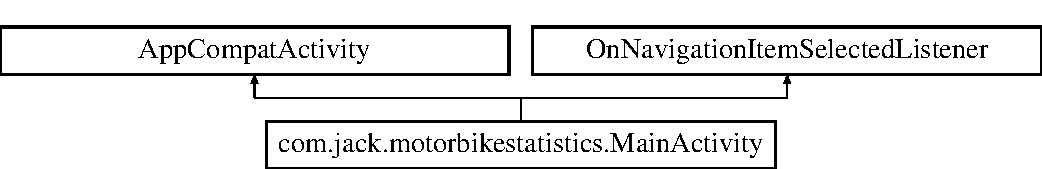
\includegraphics[height=2.000000cm]{classcom_1_1jack_1_1motorbikestatistics_1_1_main_activity}
\end{center}
\end{figure}
\subsection*{Public Member Functions}
\begin{DoxyCompactItemize}
\item 
\mbox{\Hypertarget{classcom_1_1jack_1_1motorbikestatistics_1_1_main_activity_a7cc508edb3037695e1a75eb342124fbc}\label{classcom_1_1jack_1_1motorbikestatistics_1_1_main_activity_a7cc508edb3037695e1a75eb342124fbc}} 
void \hyperlink{classcom_1_1jack_1_1motorbikestatistics_1_1_main_activity_a7cc508edb3037695e1a75eb342124fbc}{on\+Back\+Pressed} ()
\begin{DoxyCompactList}\small\item\em Responsible for closing navigation drawer when back button pressed. \end{DoxyCompactList}\item 
boolean \hyperlink{classcom_1_1jack_1_1motorbikestatistics_1_1_main_activity_a38f3fc764869f436e53413ae14590872}{on\+Navigation\+Item\+Selected} (Menu\+Item item)
\begin{DoxyCompactList}\small\item\em Changes active fragment when a tab has been pressed. \end{DoxyCompactList}\end{DoxyCompactItemize}
\subsection*{Protected Member Functions}
\begin{DoxyCompactItemize}
\item 
void \hyperlink{classcom_1_1jack_1_1motorbikestatistics_1_1_main_activity_a69fd97053d686c295dc2c58d5c4ffb79}{on\+Create} (Bundle saved\+Instance\+State)
\begin{DoxyCompactList}\small\item\em Function called when main activity is loaded. \end{DoxyCompactList}\end{DoxyCompactItemize}
\subsection*{Static Private Attributes}
\begin{DoxyCompactItemize}
\item 
\mbox{\Hypertarget{classcom_1_1jack_1_1motorbikestatistics_1_1_main_activity_a6b63eb4aa15fd17f95f5d717e0e63108}\label{classcom_1_1jack_1_1motorbikestatistics_1_1_main_activity_a6b63eb4aa15fd17f95f5d717e0e63108}} 
static final String \hyperlink{classcom_1_1jack_1_1motorbikestatistics_1_1_main_activity_a6b63eb4aa15fd17f95f5d717e0e63108}{R\+E\+A\+L\+T\+I\+M\+E\+\_\+\+C\+H\+AR} = \char`\"{}1\char`\"{}
\begin{DoxyCompactList}\small\item\em Command for switching to realtime logging. \end{DoxyCompactList}\item 
\mbox{\Hypertarget{classcom_1_1jack_1_1motorbikestatistics_1_1_main_activity_a853e8df63cac245f60ef82edaaa7ee31}\label{classcom_1_1jack_1_1motorbikestatistics_1_1_main_activity_a853e8df63cac245f60ef82edaaa7ee31}} 
static final String \hyperlink{classcom_1_1jack_1_1motorbikestatistics_1_1_main_activity_a853e8df63cac245f60ef82edaaa7ee31}{L\+I\+S\+T\+\_\+\+S\+A\+V\+E\+D\+\_\+\+C\+H\+AR} = \char`\"{}2\char`\"{}
\begin{DoxyCompactList}\small\item\em Command for loading all saved trip details. \end{DoxyCompactList}\item 
\mbox{\Hypertarget{classcom_1_1jack_1_1motorbikestatistics_1_1_main_activity_a5d506143e7f082edf2078025c00f3715}\label{classcom_1_1jack_1_1motorbikestatistics_1_1_main_activity_a5d506143e7f082edf2078025c00f3715}} 
static \hyperlink{classcom_1_1jack_1_1motorbikestatistics_1_1_realtime_fragment}{Realtime\+Fragment} \hyperlink{classcom_1_1jack_1_1motorbikestatistics_1_1_main_activity_a5d506143e7f082edf2078025c00f3715}{rt\+Fragment} = null
\begin{DoxyCompactList}\small\item\em UI fragment for realtime statistic display. \end{DoxyCompactList}\item 
\mbox{\Hypertarget{classcom_1_1jack_1_1motorbikestatistics_1_1_main_activity_ac2ac0c852d3352efd6368ee550ef3c3c}\label{classcom_1_1jack_1_1motorbikestatistics_1_1_main_activity_ac2ac0c852d3352efd6368ee550ef3c3c}} 
static \hyperlink{classcom_1_1jack_1_1motorbikestatistics_1_1_load_device_fragment}{Load\+Device\+Fragment} \hyperlink{classcom_1_1jack_1_1motorbikestatistics_1_1_main_activity_ac2ac0c852d3352efd6368ee550ef3c3c}{ld\+Fragment} = null
\begin{DoxyCompactList}\small\item\em UI fragment for loading previous trips. \end{DoxyCompactList}\item 
\mbox{\Hypertarget{classcom_1_1jack_1_1motorbikestatistics_1_1_main_activity_a2802ad16b5fdba42834d1b31e255dd96}\label{classcom_1_1jack_1_1motorbikestatistics_1_1_main_activity_a2802ad16b5fdba42834d1b31e255dd96}} 
static \hyperlink{classcom_1_1jack_1_1motorbikestatistics_1_1_pair_device_fragment}{Pair\+Device\+Fragment} \hyperlink{classcom_1_1jack_1_1motorbikestatistics_1_1_main_activity_a2802ad16b5fdba42834d1b31e255dd96}{pd\+Fragment} = null
\begin{DoxyCompactList}\small\item\em UI fragment for pairing to a logging device. \end{DoxyCompactList}\end{DoxyCompactItemize}


\subsection{Detailed Description}
Main activity class for fragment navigation. 

\subsection{Member Function Documentation}
\mbox{\Hypertarget{classcom_1_1jack_1_1motorbikestatistics_1_1_main_activity_a69fd97053d686c295dc2c58d5c4ffb79}\label{classcom_1_1jack_1_1motorbikestatistics_1_1_main_activity_a69fd97053d686c295dc2c58d5c4ffb79}} 
\index{com\+::jack\+::motorbikestatistics\+::\+Main\+Activity@{com\+::jack\+::motorbikestatistics\+::\+Main\+Activity}!on\+Create@{on\+Create}}
\index{on\+Create@{on\+Create}!com\+::jack\+::motorbikestatistics\+::\+Main\+Activity@{com\+::jack\+::motorbikestatistics\+::\+Main\+Activity}}
\subsubsection{\texorpdfstring{on\+Create()}{onCreate()}}
{\footnotesize\ttfamily void com.\+jack.\+motorbikestatistics.\+Main\+Activity.\+on\+Create (\begin{DoxyParamCaption}\item[{Bundle}]{saved\+Instance\+State }\end{DoxyParamCaption})\hspace{0.3cm}{\ttfamily [inline]}, {\ttfamily [protected]}}



Function called when main activity is loaded. 

Procedure is called when application is first started, sets up UI and creates relevant fragments.


\begin{DoxyParams}{Parameters}
{\em saved\+Instance\+State} & -\/ Information holding last previous state. \\
\hline
\end{DoxyParams}

\begin{DoxyCode}
55                                                        \{
56         super.onCreate(savedInstanceState);
57         setContentView(R.layout.activity\_main);
58 
59         Toolbar toolbar = (Toolbar) findViewById(R.id.toolbar);
60         setSupportActionBar(toolbar);
61 
62         DrawerLayout drawer = (DrawerLayout) findViewById(R.id.drawer\_layout);
63         ActionBarDrawerToggle toggle = \textcolor{keyword}{new} ActionBarDrawerToggle(
64                 \textcolor{keyword}{this}, drawer, toolbar, R.string.navigation\_drawer\_open, R.string.navigation\_drawer\_close);
65         drawer.setDrawerListener(toggle);
66         toggle.syncState();
67 
68         NavigationView navigationView = (NavigationView) findViewById(R.id.nav\_view);
69         navigationView.setNavigationItemSelectedListener(\textcolor{keyword}{this});
70 
71         \textcolor{comment}{/* Create our fragments for different sections of UI */}
72         \hyperlink{classcom_1_1jack_1_1motorbikestatistics_1_1_main_activity_a5d506143e7f082edf2078025c00f3715}{rtFragment} = \textcolor{keyword}{new} RealtimeFragment();
73         \hyperlink{classcom_1_1jack_1_1motorbikestatistics_1_1_main_activity_ac2ac0c852d3352efd6368ee550ef3c3c}{ldFragment} = \textcolor{keyword}{new} LoadDeviceFragment();
74         \hyperlink{classcom_1_1jack_1_1motorbikestatistics_1_1_main_activity_a2802ad16b5fdba42834d1b31e255dd96}{pdFragment} = \textcolor{keyword}{new} PairDeviceFragment();
75     \}
\end{DoxyCode}
\mbox{\Hypertarget{classcom_1_1jack_1_1motorbikestatistics_1_1_main_activity_a38f3fc764869f436e53413ae14590872}\label{classcom_1_1jack_1_1motorbikestatistics_1_1_main_activity_a38f3fc764869f436e53413ae14590872}} 
\index{com\+::jack\+::motorbikestatistics\+::\+Main\+Activity@{com\+::jack\+::motorbikestatistics\+::\+Main\+Activity}!on\+Navigation\+Item\+Selected@{on\+Navigation\+Item\+Selected}}
\index{on\+Navigation\+Item\+Selected@{on\+Navigation\+Item\+Selected}!com\+::jack\+::motorbikestatistics\+::\+Main\+Activity@{com\+::jack\+::motorbikestatistics\+::\+Main\+Activity}}
\subsubsection{\texorpdfstring{on\+Navigation\+Item\+Selected()}{onNavigationItemSelected()}}
{\footnotesize\ttfamily boolean com.\+jack.\+motorbikestatistics.\+Main\+Activity.\+on\+Navigation\+Item\+Selected (\begin{DoxyParamCaption}\item[{Menu\+Item}]{item }\end{DoxyParamCaption})\hspace{0.3cm}{\ttfamily [inline]}}



Changes active fragment when a tab has been pressed. 

Responsible for changing to the new chosen fragment on the UI. Opening of realtime and loaddevice fragments not possible when not connected to the logging device.

Method also responsible for change system state machine on the logging device, this is done by transmitting command code.


\begin{DoxyParams}{Parameters}
{\em item} & -\/ New selected fragment/tab to display. \\
\hline
\end{DoxyParams}


References com.\+jack.\+motorbikestatistics.\+Pair\+Device\+Fragment.\+get\+B\+T\+Connection(), com.\+jack.\+motorbikestatistics.\+B\+T\+Connection.\+is\+Connected(), com.\+jack.\+motorbikestatistics.\+Main\+Activity.\+ld\+Fragment, com.\+jack.\+motorbikestatistics.\+Main\+Activity.\+pd\+Fragment, com.\+jack.\+motorbikestatistics.\+Main\+Activity.\+rt\+Fragment, com.\+jack.\+motorbikestatistics.\+Load\+Device\+Fragment.\+R\+X\+Handler, com.\+jack.\+motorbikestatistics.\+Load\+Device\+Fragment.\+set\+B\+T\+Connection(), com.\+jack.\+motorbikestatistics.\+B\+T\+Connection.\+set\+R\+X\+Handler(), and com.\+jack.\+motorbikestatistics.\+B\+T\+Connection.\+tx\+Handler.


\begin{DoxyCode}
105                                                            \{
106 
107         Fragment activeFragment = null;
108 
109         \textcolor{comment}{/* Handle navigation view clicks here */}
110         FragmentManager fragmentManager = getFragmentManager();
111         \textcolor{keywordtype}{int} \textcolor{keywordtype}{id} = item.getItemId();
112 
113         \textcolor{keywordflow}{switch} (\textcolor{keywordtype}{id}) \{
114             \textcolor{keywordflow}{case} R.id.nav\_realtime: \{
115                 \textcolor{comment}{/* Get our bluetooth connection from pairing fragment */}
116                 BTConnection btConn = \hyperlink{classcom_1_1jack_1_1motorbikestatistics_1_1_main_activity_a2802ad16b5fdba42834d1b31e255dd96}{pdFragment}.\hyperlink{classcom_1_1jack_1_1motorbikestatistics_1_1_pair_device_fragment_a32debe1358d94bb1c972137f60d1aa36}{getBTConnection}();
117 
118                 \textcolor{keywordflow}{if} (btConn != null && btConn.isConnected()) \{
119                     \textcolor{comment}{/* We set our RX handler and also send our command to indicate mode change */}
120                     btConn.\hyperlink{classcom_1_1jack_1_1motorbikestatistics_1_1_b_t_connection_aae8ee75e78f5beff98572bf3b13a60b8}{setRXHandler}(\hyperlink{classcom_1_1jack_1_1motorbikestatistics_1_1_main_activity_a5d506143e7f082edf2078025c00f3715}{rtFragment}.RXHandler);
121                     Message message = \textcolor{keyword}{new} Message();
122                     message.obj = (String) \hyperlink{classcom_1_1jack_1_1motorbikestatistics_1_1_main_activity_a6b63eb4aa15fd17f95f5d717e0e63108}{REALTIME\_CHAR};
123                     message.setTarget(btConn.txHandler);
124                     message.sendToTarget();
125 
126                     \textcolor{comment}{/* Change to our new active fragment */}
127                     activeFragment = \hyperlink{classcom_1_1jack_1_1motorbikestatistics_1_1_main_activity_a5d506143e7f082edf2078025c00f3715}{rtFragment};
128                 \} \textcolor{keywordflow}{else} \{
129                     \textcolor{comment}{/* Indicate that we are not connected to device */}
130                     View rootView = findViewById(R.id.content\_main);
131                     Snackbar.make(rootView, \textcolor{stringliteral}{"Please connect to a device first."}, Snackbar.LENGTH\_LONG)
132                             .setAction(\textcolor{stringliteral}{"Action"}, null).show();
133                 \}
134                 \textcolor{keywordflow}{break};
135             \}
136 
137             \textcolor{keywordflow}{case} R.id.nav\_loaddevice: \{
138                 \textcolor{comment}{/* Get our bluetooth connection from pairing fragment */}
139                 BTConnection btConn = \hyperlink{classcom_1_1jack_1_1motorbikestatistics_1_1_main_activity_a2802ad16b5fdba42834d1b31e255dd96}{pdFragment}.\hyperlink{classcom_1_1jack_1_1motorbikestatistics_1_1_pair_device_fragment_a32debe1358d94bb1c972137f60d1aa36}{getBTConnection}();
140 
141                 \textcolor{keywordflow}{if} (btConn != null && btConn.isConnected()) \{
142                     \textcolor{comment}{/* We set our RX handler and also send our command to indicate mode change */}
143                     \hyperlink{classcom_1_1jack_1_1motorbikestatistics_1_1_main_activity_ac2ac0c852d3352efd6368ee550ef3c3c}{ldFragment}.\hyperlink{classcom_1_1jack_1_1motorbikestatistics_1_1_load_device_fragment_aec66dc5fd944098de78ace4175fca5b6}{setBTConnection}(btConn);
144 
145                     btConn.setRXHandler(\hyperlink{classcom_1_1jack_1_1motorbikestatistics_1_1_main_activity_ac2ac0c852d3352efd6368ee550ef3c3c}{ldFragment}.\hyperlink{classcom_1_1jack_1_1motorbikestatistics_1_1_load_device_fragment_a7c26c8686c290d8766b051f31473d716}{RXHandler});
146                     Message message = \textcolor{keyword}{new} Message();
147                     message.obj = (String) \hyperlink{classcom_1_1jack_1_1motorbikestatistics_1_1_main_activity_a853e8df63cac245f60ef82edaaa7ee31}{LIST\_SAVED\_CHAR};
148                     message.setTarget(btConn.txHandler);
149                     message.sendToTarget();
150 
151                     \textcolor{comment}{/* Change to our new active fragment */}
152                     activeFragment = \hyperlink{classcom_1_1jack_1_1motorbikestatistics_1_1_main_activity_ac2ac0c852d3352efd6368ee550ef3c3c}{ldFragment};
153                 \} \textcolor{keywordflow}{else} \{
154                     \textcolor{comment}{/* Indicate that we are not connected to device */}
155                     View rootView = findViewById(R.id.content\_main);
156                     Snackbar.make(rootView, \textcolor{stringliteral}{"Please connect to a device first."}, Snackbar.LENGTH\_LONG)
157                             .setAction(\textcolor{stringliteral}{"Action"}, null).show();
158                 \}
159                 \textcolor{keywordflow}{break};
160             \}
161 
162             \textcolor{keywordflow}{case} R.id.nav\_pairdevice: \{
163                 activeFragment = \hyperlink{classcom_1_1jack_1_1motorbikestatistics_1_1_main_activity_a2802ad16b5fdba42834d1b31e255dd96}{pdFragment};
164             \}
165 
166         \}
167 
168         \textcolor{keywordflow}{if} (activeFragment != null) \{
169             \textcolor{comment}{/* Replaces content frame with newly selected one */}
170             fragmentManager.beginTransaction()
171                     .replace(R.id.content\_frame, activeFragment)
172                     .commit();
173         \}
174 
175         DrawerLayout drawer = (DrawerLayout) findViewById(R.id.drawer\_layout);
176         drawer.closeDrawer(GravityCompat.START);
177         \textcolor{keywordflow}{return} (activeFragment != null);
178     \}
\end{DoxyCode}


The documentation for this class was generated from the following file\+:\begin{DoxyCompactItemize}
\item 
android-\/app/app/src/main/java/com/jack/motorbikestatistics/\hyperlink{_main_activity_8java}{Main\+Activity.\+java}\end{DoxyCompactItemize}

\hypertarget{classcom_1_1jack_1_1motorbikestatistics_1_1_maps_activity}{}\section{com.\+jack.\+motorbikestatistics.\+Maps\+Activity Class Reference}
\label{classcom_1_1jack_1_1motorbikestatistics_1_1_maps_activity}\index{com.\+jack.\+motorbikestatistics.\+Maps\+Activity@{com.\+jack.\+motorbikestatistics.\+Maps\+Activity}}


Maps activity class for displaying map data.  


Inheritance diagram for com.\+jack.\+motorbikestatistics.\+Maps\+Activity\+:\begin{figure}[H]
\begin{center}
\leavevmode
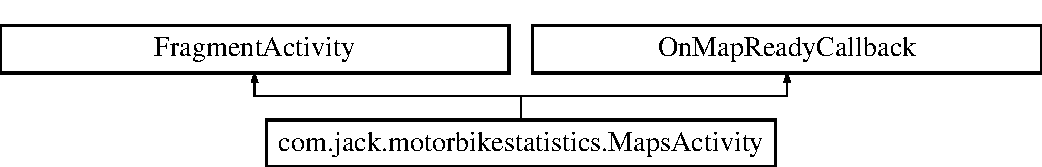
\includegraphics[height=2.000000cm]{classcom_1_1jack_1_1motorbikestatistics_1_1_maps_activity}
\end{center}
\end{figure}
\subsection*{Classes}
\begin{DoxyCompactItemize}
\item 
class \hyperlink{classcom_1_1jack_1_1motorbikestatistics_1_1_maps_activity_1_1_statistic_window_adapter}{Statistic\+Window\+Adapter}
\begin{DoxyCompactList}\small\item\em Adapter used for displaying statistics at a certain marker that user has clicked on. \end{DoxyCompactList}\end{DoxyCompactItemize}
\subsection*{Public Member Functions}
\begin{DoxyCompactItemize}
\item 
void \hyperlink{classcom_1_1jack_1_1motorbikestatistics_1_1_maps_activity_aefa35b548b2f39bb46b2cb5024be383c}{on\+Map\+Ready} (Google\+Map google\+Map)
\begin{DoxyCompactList}\small\item\em Manipulates the map once available. \end{DoxyCompactList}\end{DoxyCompactItemize}
\subsection*{Protected Member Functions}
\begin{DoxyCompactItemize}
\item 
void \hyperlink{classcom_1_1jack_1_1motorbikestatistics_1_1_maps_activity_afd23eb0cf651de276a9b85bb5fa609b8}{on\+Create} (Bundle saved\+Instance\+State)
\begin{DoxyCompactList}\small\item\em Fills our maps array with points to plot on the map. \end{DoxyCompactList}\end{DoxyCompactItemize}
\subsection*{Private Member Functions}
\begin{DoxyCompactItemize}
\item 
boolean \hyperlink{classcom_1_1jack_1_1motorbikestatistics_1_1_maps_activity_a0c72fcb79424420c3477add9ba6ab447}{get\+J\+S\+O\+N\+Objects} ()
\begin{DoxyCompactList}\small\item\em Gets point data and convert to array of J\+S\+ON objects. \end{DoxyCompactList}\item 
J\+S\+O\+N\+Object \hyperlink{classcom_1_1jack_1_1motorbikestatistics_1_1_maps_activity_ae5478e56dfb617433d0dfaeb94a403c7}{find\+J\+S\+O\+N\+By\+Lat\+Lng} (Lat\+Lng position)
\begin{DoxyCompactList}\small\item\em Finds J\+S\+O\+N\+Object from Array\+List via L\+A\+T/\+L\+NG coordinates. \end{DoxyCompactList}\item 
float \hyperlink{classcom_1_1jack_1_1motorbikestatistics_1_1_maps_activity_af4feb7617c02a59c62d6e9257914e997}{calc\+Distance} (Lat\+Lng start, Lat\+Lng end)
\begin{DoxyCompactList}\small\item\em Calculates the absolute distance between two points. \end{DoxyCompactList}\end{DoxyCompactItemize}
\subsection*{Private Attributes}
\begin{DoxyCompactItemize}
\item 
\mbox{\Hypertarget{classcom_1_1jack_1_1motorbikestatistics_1_1_maps_activity_aaace5219464acf3df9ac5e9ce913eef5}\label{classcom_1_1jack_1_1motorbikestatistics_1_1_maps_activity_aaace5219464acf3df9ac5e9ce913eef5}} 
Google\+Map \hyperlink{classcom_1_1jack_1_1motorbikestatistics_1_1_maps_activity_aaace5219464acf3df9ac5e9ce913eef5}{m\+Map}
\begin{DoxyCompactList}\small\item\em Google maps object for plotting. \end{DoxyCompactList}\item 
\mbox{\Hypertarget{classcom_1_1jack_1_1motorbikestatistics_1_1_maps_activity_aaed26c36e08dad942830ab52d9d75d2e}\label{classcom_1_1jack_1_1motorbikestatistics_1_1_maps_activity_aaed26c36e08dad942830ab52d9d75d2e}} 
Array\+List$<$ J\+S\+O\+N\+Object $>$ \hyperlink{classcom_1_1jack_1_1motorbikestatistics_1_1_maps_activity_aaed26c36e08dad942830ab52d9d75d2e}{json\+List} = new Array\+List$<$J\+S\+O\+N\+Object$>$()
\begin{DoxyCompactList}\small\item\em Array\+List holding all trip data. \end{DoxyCompactList}\end{DoxyCompactItemize}


\subsection{Detailed Description}
Maps activity class for displaying map data. 

\subsection{Member Function Documentation}
\mbox{\Hypertarget{classcom_1_1jack_1_1motorbikestatistics_1_1_maps_activity_afd23eb0cf651de276a9b85bb5fa609b8}\label{classcom_1_1jack_1_1motorbikestatistics_1_1_maps_activity_afd23eb0cf651de276a9b85bb5fa609b8}} 
\index{com\+::jack\+::motorbikestatistics\+::\+Maps\+Activity@{com\+::jack\+::motorbikestatistics\+::\+Maps\+Activity}!on\+Create@{on\+Create}}
\index{on\+Create@{on\+Create}!com\+::jack\+::motorbikestatistics\+::\+Maps\+Activity@{com\+::jack\+::motorbikestatistics\+::\+Maps\+Activity}}
\subsubsection{\texorpdfstring{on\+Create()}{onCreate()}}
{\footnotesize\ttfamily void com.\+jack.\+motorbikestatistics.\+Maps\+Activity.\+on\+Create (\begin{DoxyParamCaption}\item[{Bundle}]{saved\+Instance\+State }\end{DoxyParamCaption})\hspace{0.3cm}{\ttfamily [inline]}, {\ttfamily [protected]}}



Fills our maps array with points to plot on the map. 

Called when maps activity is first started. Responsible for making sure we have points to plot.


\begin{DoxyParams}{Parameters}
{\em saved\+Instance\+State} & -\/ Information holding last previous state. \\
\hline
\end{DoxyParams}


References com.\+jack.\+motorbikestatistics.\+Maps\+Activity.\+get\+J\+S\+O\+N\+Objects().


\begin{DoxyCode}
56                                                        \{
57         super.onCreate(savedInstanceState);
58         setContentView(R.layout.activity\_maps);
59         \textcolor{comment}{// Obtain the SupportMapFragment and get notified when the map is ready to be used.}
60         SupportMapFragment mapFragment = (SupportMapFragment) getSupportFragmentManager()
61                 .findFragmentById(R.id.map);
62 
63         \hyperlink{classcom_1_1jack_1_1motorbikestatistics_1_1_maps_activity_a0c72fcb79424420c3477add9ba6ab447}{getJSONObjects}();
64 
65         mapFragment.getMapAsync(\textcolor{keyword}{this});
66     \}
\end{DoxyCode}
\mbox{\Hypertarget{classcom_1_1jack_1_1motorbikestatistics_1_1_maps_activity_a0c72fcb79424420c3477add9ba6ab447}\label{classcom_1_1jack_1_1motorbikestatistics_1_1_maps_activity_a0c72fcb79424420c3477add9ba6ab447}} 
\index{com\+::jack\+::motorbikestatistics\+::\+Maps\+Activity@{com\+::jack\+::motorbikestatistics\+::\+Maps\+Activity}!get\+J\+S\+O\+N\+Objects@{get\+J\+S\+O\+N\+Objects}}
\index{get\+J\+S\+O\+N\+Objects@{get\+J\+S\+O\+N\+Objects}!com\+::jack\+::motorbikestatistics\+::\+Maps\+Activity@{com\+::jack\+::motorbikestatistics\+::\+Maps\+Activity}}
\subsubsection{\texorpdfstring{get\+J\+S\+O\+N\+Objects()}{getJSONObjects()}}
{\footnotesize\ttfamily boolean com.\+jack.\+motorbikestatistics.\+Maps\+Activity.\+get\+J\+S\+O\+N\+Objects (\begin{DoxyParamCaption}{ }\end{DoxyParamCaption})\hspace{0.3cm}{\ttfamily [inline]}, {\ttfamily [private]}}



Gets point data and convert to array of J\+S\+ON objects. 

Gets an arraylist of strings passed via a bundle to this activity. These strings are there converted back to J\+S\+ON objects which will be used for plotting. The reason for not passing straight J\+S\+ON objects is because they are not serializable and passable between activities.

\begin{DoxyReturn}{Returns}
boolean -\/ Whether all objects were able to be created. 
\end{DoxyReturn}

\begin{DoxyCode}
80     \{
81         \textcolor{keywordtype}{boolean} result = \textcolor{keyword}{true};
82 
83         \textcolor{comment}{/*}
84 \textcolor{comment}{         * Get our serialized arrayList of jsonStrings}
85 \textcolor{comment}{         * then convert them back to jsonObjects}
86 \textcolor{comment}{         */}
87         ArrayList<String> jsonStrings = (ArrayList<String>)getIntent().getSerializableExtra(\textcolor{stringliteral}{"JSONList"});
88         \textcolor{keywordflow}{for} (\textcolor{keywordtype}{int} i = 0; i < jsonStrings.size(); i++)
89         \{
90             \textcolor{keywordflow}{try}
91             \{
92                 JSONObject jsonObject = \textcolor{keyword}{new} JSONObject(jsonStrings.get(i));
93                 \hyperlink{classcom_1_1jack_1_1motorbikestatistics_1_1_maps_activity_aaed26c36e08dad942830ab52d9d75d2e}{jsonList}.add(jsonObject);
94             \}
95             \textcolor{keywordflow}{catch} (JSONException e)
96             \{
97                 result = \textcolor{keyword}{false};
98             \}
99         \}
100 
101         \textcolor{keywordflow}{return} result;
102     \}
\end{DoxyCode}
\mbox{\Hypertarget{classcom_1_1jack_1_1motorbikestatistics_1_1_maps_activity_ae5478e56dfb617433d0dfaeb94a403c7}\label{classcom_1_1jack_1_1motorbikestatistics_1_1_maps_activity_ae5478e56dfb617433d0dfaeb94a403c7}} 
\index{com\+::jack\+::motorbikestatistics\+::\+Maps\+Activity@{com\+::jack\+::motorbikestatistics\+::\+Maps\+Activity}!find\+J\+S\+O\+N\+By\+Lat\+Lng@{find\+J\+S\+O\+N\+By\+Lat\+Lng}}
\index{find\+J\+S\+O\+N\+By\+Lat\+Lng@{find\+J\+S\+O\+N\+By\+Lat\+Lng}!com\+::jack\+::motorbikestatistics\+::\+Maps\+Activity@{com\+::jack\+::motorbikestatistics\+::\+Maps\+Activity}}
\subsubsection{\texorpdfstring{find\+J\+S\+O\+N\+By\+Lat\+Lng()}{findJSONByLatLng()}}
{\footnotesize\ttfamily J\+S\+O\+N\+Object com.\+jack.\+motorbikestatistics.\+Maps\+Activity.\+find\+J\+S\+O\+N\+By\+Lat\+Lng (\begin{DoxyParamCaption}\item[{Lat\+Lng}]{position }\end{DoxyParamCaption})\hspace{0.3cm}{\ttfamily [inline]}, {\ttfamily [private]}}



Finds J\+S\+O\+N\+Object from Array\+List via L\+A\+T/\+L\+NG coordinates. 


\begin{DoxyParams}{Parameters}
{\em position} & -\/ Latitude and Longitude position. \\
\hline
\end{DoxyParams}
\begin{DoxyReturn}{Returns}
J\+S\+O\+N\+Object -\/ The found J\+S\+ON object. 
\end{DoxyReturn}


References gps\+J\+S\+ON.


\begin{DoxyCode}
110                                                          \{
111         JSONObject result = null;
112 
113         \textcolor{keywordflow}{for} (\textcolor{keywordtype}{int} i = 0; i < \hyperlink{classcom_1_1jack_1_1motorbikestatistics_1_1_maps_activity_aaed26c36e08dad942830ab52d9d75d2e}{jsonList}.size(); i++) \{
114             JSONObject tmpJSON = \hyperlink{classcom_1_1jack_1_1motorbikestatistics_1_1_maps_activity_aaed26c36e08dad942830ab52d9d75d2e}{jsonList}.get(i);
115 
116             \textcolor{keywordflow}{try} \{
117                 JSONObject \hyperlink{logging-device_8ino_a548727e041a5cd3db91bdbd0ccd71e30}{gpsJSON} = tmpJSON.getJSONObject(\textcolor{stringliteral}{"gps"});
118 
119                 Double latitude = gpsJSON.getDouble(\textcolor{stringliteral}{"lat"});
120                 Double longitude = gpsJSON.getDouble(\textcolor{stringliteral}{"lng"});
121 
122                 \textcolor{comment}{/* Check to see if latitude and logitudes match */}
123                 \textcolor{keywordflow}{if} ((latitude == position.latitude) && (longitude == position.longitude)) \{
124                     result = tmpJSON;
125                     \textcolor{keywordflow}{break};
126                 \}
127 
128             \} \textcolor{keywordflow}{catch} (JSONException e) \{
129                 \textcolor{comment}{/* Do nothing */}
130             \}
131         \}
132 
133         \textcolor{keywordflow}{return} result;
134     \}
\end{DoxyCode}
\mbox{\Hypertarget{classcom_1_1jack_1_1motorbikestatistics_1_1_maps_activity_af4feb7617c02a59c62d6e9257914e997}\label{classcom_1_1jack_1_1motorbikestatistics_1_1_maps_activity_af4feb7617c02a59c62d6e9257914e997}} 
\index{com\+::jack\+::motorbikestatistics\+::\+Maps\+Activity@{com\+::jack\+::motorbikestatistics\+::\+Maps\+Activity}!calc\+Distance@{calc\+Distance}}
\index{calc\+Distance@{calc\+Distance}!com\+::jack\+::motorbikestatistics\+::\+Maps\+Activity@{com\+::jack\+::motorbikestatistics\+::\+Maps\+Activity}}
\subsubsection{\texorpdfstring{calc\+Distance()}{calcDistance()}}
{\footnotesize\ttfamily float com.\+jack.\+motorbikestatistics.\+Maps\+Activity.\+calc\+Distance (\begin{DoxyParamCaption}\item[{Lat\+Lng}]{start,  }\item[{Lat\+Lng}]{end }\end{DoxyParamCaption})\hspace{0.3cm}{\ttfamily [inline]}, {\ttfamily [private]}}



Calculates the absolute distance between two points. 

Distance is as the crow flys and not via streets etc. 
\begin{DoxyParams}{Parameters}
{\em start} & -\/ Start position. \\
\hline
{\em end} & -\/ End position. \\
\hline
\end{DoxyParams}
\begin{DoxyReturn}{Returns}
flaot -\/ Distance between points in metres. 
\end{DoxyReturn}

\begin{DoxyCode}
145     \{
146         \textcolor{keywordtype}{float}[] results = \textcolor{keyword}{new} \textcolor{keywordtype}{float}[1];
147 
148         Location.distanceBetween(start.latitude, start.longitude, end.latitude, end.longitude, results);
149         \textcolor{keywordflow}{return} results[0];
150     \}
\end{DoxyCode}
\mbox{\Hypertarget{classcom_1_1jack_1_1motorbikestatistics_1_1_maps_activity_aefa35b548b2f39bb46b2cb5024be383c}\label{classcom_1_1jack_1_1motorbikestatistics_1_1_maps_activity_aefa35b548b2f39bb46b2cb5024be383c}} 
\index{com\+::jack\+::motorbikestatistics\+::\+Maps\+Activity@{com\+::jack\+::motorbikestatistics\+::\+Maps\+Activity}!on\+Map\+Ready@{on\+Map\+Ready}}
\index{on\+Map\+Ready@{on\+Map\+Ready}!com\+::jack\+::motorbikestatistics\+::\+Maps\+Activity@{com\+::jack\+::motorbikestatistics\+::\+Maps\+Activity}}
\subsubsection{\texorpdfstring{on\+Map\+Ready()}{onMapReady()}}
{\footnotesize\ttfamily void com.\+jack.\+motorbikestatistics.\+Maps\+Activity.\+on\+Map\+Ready (\begin{DoxyParamCaption}\item[{Google\+Map}]{google\+Map }\end{DoxyParamCaption})\hspace{0.3cm}{\ttfamily [inline]}}



Manipulates the map once available. 

This callback is triggered when the map is ready to be used. This is where we can add markers or lines.

If Google Play services is not installed on the device, the user will be prompted to install it inside the Support\+Map\+Fragment. This method will only be triggered once the user has installed Google Play services and returned to the app.


\begin{DoxyParams}{Parameters}
{\em google\+Map} & -\/ Our map object ready to manipulate. \\
\hline
\end{DoxyParams}


References com.\+jack.\+motorbikestatistics.\+Maps\+Activity.\+calc\+Distance(), and gps\+J\+S\+ON.


\begin{DoxyCode}
165                                                 \{
166         \hyperlink{classcom_1_1jack_1_1motorbikestatistics_1_1_maps_activity_aaace5219464acf3df9ac5e9ce913eef5}{mMap} = googleMap;
167 
168         \hyperlink{classcom_1_1jack_1_1motorbikestatistics_1_1_maps_activity_aaace5219464acf3df9ac5e9ce913eef5}{mMap}.setMapType(GoogleMap.MAP\_TYPE\_HYBRID);
169 
170         \textcolor{comment}{/* Set our info window adapter class that is shown when marker clicked */}
171         \hyperlink{classcom_1_1jack_1_1motorbikestatistics_1_1_maps_activity_aaace5219464acf3df9ac5e9ce913eef5}{mMap}.setInfoWindowAdapter(\textcolor{keyword}{new} StatisticWindowAdapter());
172 
173         \textcolor{comment}{/* If we have no data don't bother plotting points */}
174         \textcolor{keywordflow}{if} (\hyperlink{classcom_1_1jack_1_1motorbikestatistics_1_1_maps_activity_aaed26c36e08dad942830ab52d9d75d2e}{jsonList}.size() != 0)
175         \{
176             \textcolor{comment}{/* lineOpts will store our route */}
177             PolylineOptions lineOpts = \textcolor{keyword}{new} PolylineOptions();
178             lineOpts.color(Color.parseColor( \textcolor{stringliteral}{"#CC0000FF"}));
179             lineOpts.width(5);
180             lineOpts.visible(\textcolor{keyword}{true});
181 
182             \textcolor{keywordflow}{try}
183             \{
184                 LatLng lastMarker = null;
185 
186                 \textcolor{comment}{/* Plot every point in the our JSONObject array */}
187                 \textcolor{keywordflow}{for} (\textcolor{keywordtype}{int} i = 0; i < \hyperlink{classcom_1_1jack_1_1motorbikestatistics_1_1_maps_activity_aaed26c36e08dad942830ab52d9d75d2e}{jsonList}.size(); i++)
188                 \{
189                     JSONObject rootJSON = \hyperlink{classcom_1_1jack_1_1motorbikestatistics_1_1_maps_activity_aaed26c36e08dad942830ab52d9d75d2e}{jsonList}.get(i);
190                     JSONObject \hyperlink{logging-device_8ino_a548727e041a5cd3db91bdbd0ccd71e30}{gpsJSON} = rootJSON.getJSONObject(\textcolor{stringliteral}{"gps"});
191 
192                     Double lat = gpsJSON.getDouble(\textcolor{stringliteral}{"lat"});
193                     Double lng = gpsJSON.getDouble(\textcolor{stringliteral}{"lng"});
194                     LatLng location = \textcolor{keyword}{new} LatLng(lat, lng);
195 
196                     \textcolor{comment}{/* Add this location to our trip line */}
197                     lineOpts.add(location);
198 
199                     \textcolor{comment}{/*}
200 \textcolor{comment}{                     * Check if distance between this point and}
201 \textcolor{comment}{                     * last marker is greater than 5m otherwise don't add marker.}
202 \textcolor{comment}{                     * Adding markers every 5 metres prevents the map being spammed with}
203 \textcolor{comment}{                     * thousands of readings.}
204 \textcolor{comment}{                     */}
205                     \textcolor{keywordflow}{if} ((lastMarker == null) || (\hyperlink{classcom_1_1jack_1_1motorbikestatistics_1_1_maps_activity_af4feb7617c02a59c62d6e9257914e997}{calcDistance}(location, lastMarker) > 5))
206                     \{
207                         \textcolor{comment}{/* Only add a marker if the gps data is valid */}
208                         \textcolor{keywordflow}{if} (gpsJSON.getBoolean(\textcolor{stringliteral}{"gps\_valid"}) == \textcolor{keyword}{true}) \{
209                             MarkerOptions markerOptions = \textcolor{keyword}{new} MarkerOptions();
210                             markerOptions.position(location);
211                             markerOptions.title(\textcolor{stringliteral}{"Reading: "} + i);
212 
213                             \hyperlink{classcom_1_1jack_1_1motorbikestatistics_1_1_maps_activity_aaace5219464acf3df9ac5e9ce913eef5}{mMap}.addMarker(markerOptions);
214 
215                             lastMarker = location;
216 
217                             \textcolor{comment}{/* Changes camera to point to newest marker */}
218                             \hyperlink{classcom_1_1jack_1_1motorbikestatistics_1_1_maps_activity_aaace5219464acf3df9ac5e9ce913eef5}{mMap}.animateCamera(CameraUpdateFactory.newLatLngZoom(location, 12));
219                         \}
220                     \}
221 
222                 \}
223                 \hyperlink{classcom_1_1jack_1_1motorbikestatistics_1_1_maps_activity_aaace5219464acf3df9ac5e9ce913eef5}{mMap}.addPolyline(lineOpts);
224             \}
225             \textcolor{keywordflow}{catch} (JSONException e)
226             \{
227                 \textcolor{comment}{/* Do nothing */}
228             \}
229         \}
230     \}
\end{DoxyCode}


The documentation for this class was generated from the following file\+:\begin{DoxyCompactItemize}
\item 
android-\/app/app/src/main/java/com/jack/motorbikestatistics/\hyperlink{_maps_activity_8java}{Maps\+Activity.\+java}\end{DoxyCompactItemize}

\hypertarget{class_orientation}{}\section{Orientation Class Reference}
\label{class_orientation}\index{Orientation@{Orientation}}
\subsection*{Public Member Functions}
\begin{DoxyCompactItemize}
\item 
\mbox{\Hypertarget{class_orientation_aad568a473f999c181abac46a4d832387}\label{class_orientation_aad568a473f999c181abac46a4d832387}} 
bool {\bfseries poll\+I\+MU} ()
\item 
\mbox{\Hypertarget{class_orientation_a3dbaa1ee014811c40d5b9f39b544c19b}\label{class_orientation_a3dbaa1ee014811c40d5b9f39b544c19b}} 
float {\bfseries get\+Yaw} ()
\item 
\mbox{\Hypertarget{class_orientation_a7ec1a2964fc858bbd5da22a505b087c8}\label{class_orientation_a7ec1a2964fc858bbd5da22a505b087c8}} 
float {\bfseries get\+Pitch} ()
\item 
\mbox{\Hypertarget{class_orientation_ab8923432cb8c18822b0a9ae95a5ac505}\label{class_orientation_ab8923432cb8c18822b0a9ae95a5ac505}} 
float {\bfseries get\+Roll} ()
\end{DoxyCompactItemize}


The documentation for this class was generated from the following files\+:\begin{DoxyCompactItemize}
\item 
logging-\/device/Orientation.\+h\item 
logging-\/device/Orientation.\+cpp\end{DoxyCompactItemize}

\hypertarget{classcom_1_1jack_1_1motorbikestatistics_1_1_pair_device_fragment}{}\section{com.\+jack.\+motorbikestatistics.\+Pair\+Device\+Fragment Class Reference}
\label{classcom_1_1jack_1_1motorbikestatistics_1_1_pair_device_fragment}\index{com.\+jack.\+motorbikestatistics.\+Pair\+Device\+Fragment@{com.\+jack.\+motorbikestatistics.\+Pair\+Device\+Fragment}}
Inheritance diagram for com.\+jack.\+motorbikestatistics.\+Pair\+Device\+Fragment\+:\begin{figure}[H]
\begin{center}
\leavevmode
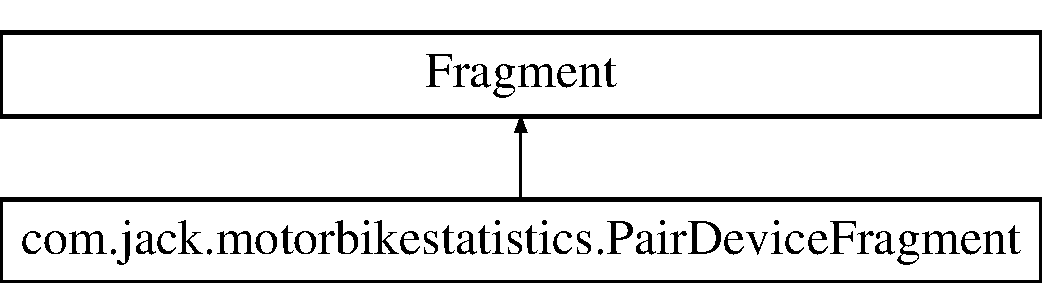
\includegraphics[height=2.000000cm]{classcom_1_1jack_1_1motorbikestatistics_1_1_pair_device_fragment}
\end{center}
\end{figure}
\subsection*{Public Member Functions}
\begin{DoxyCompactItemize}
\item 
\mbox{\Hypertarget{classcom_1_1jack_1_1motorbikestatistics_1_1_pair_device_fragment_afc7756a10d0798aa2493b9c7f6b010ad}\label{classcom_1_1jack_1_1motorbikestatistics_1_1_pair_device_fragment_afc7756a10d0798aa2493b9c7f6b010ad}} 
View {\bfseries on\+Create\+View} (Layout\+Inflater inflater, View\+Group container, Bundle saved\+Instance\+State)
\item 
\mbox{\Hypertarget{classcom_1_1jack_1_1motorbikestatistics_1_1_pair_device_fragment_a32debe1358d94bb1c972137f60d1aa36}\label{classcom_1_1jack_1_1motorbikestatistics_1_1_pair_device_fragment_a32debe1358d94bb1c972137f60d1aa36}} 
\hyperlink{classcom_1_1jack_1_1motorbikestatistics_1_1_b_t_connection}{B\+T\+Connection} {\bfseries get\+B\+T\+Connection} ()
\end{DoxyCompactItemize}
\subsection*{Public Attributes}
\begin{DoxyCompactItemize}
\item 
final Broadcast\+Receiver {\bfseries bt\+Receiver}
\item 
final Toggle\+Button.\+On\+Checked\+Change\+Listener {\bfseries toggle\+Scan\+Listener}
\item 
\mbox{\Hypertarget{classcom_1_1jack_1_1motorbikestatistics_1_1_pair_device_fragment_a4ec3a304c1da2bc4e4d2ca16da764e23}\label{classcom_1_1jack_1_1motorbikestatistics_1_1_pair_device_fragment_a4ec3a304c1da2bc4e4d2ca16da764e23}} 
final List\+View.\+On\+Item\+Click\+Listener {\bfseries list\+Item\+Listener}
\end{DoxyCompactItemize}
\subsection*{Private Member Functions}
\begin{DoxyCompactItemize}
\item 
\mbox{\Hypertarget{classcom_1_1jack_1_1motorbikestatistics_1_1_pair_device_fragment_a5be2be0c93319e38e39cf23943ab1c8c}\label{classcom_1_1jack_1_1motorbikestatistics_1_1_pair_device_fragment_a5be2be0c93319e38e39cf23943ab1c8c}} 
void {\bfseries get\+Needed\+Privileges} ()
\end{DoxyCompactItemize}
\subsection*{Private Attributes}
\begin{DoxyCompactItemize}
\item 
\mbox{\Hypertarget{classcom_1_1jack_1_1motorbikestatistics_1_1_pair_device_fragment_a11d29b376fa4676ab5852bba1369c0d0}\label{classcom_1_1jack_1_1motorbikestatistics_1_1_pair_device_fragment_a11d29b376fa4676ab5852bba1369c0d0}} 
boolean {\bfseries first\+Run} = true
\item 
\mbox{\Hypertarget{classcom_1_1jack_1_1motorbikestatistics_1_1_pair_device_fragment_a1bf1c9b623a1b9891e0d574006cf8d5f}\label{classcom_1_1jack_1_1motorbikestatistics_1_1_pair_device_fragment_a1bf1c9b623a1b9891e0d574006cf8d5f}} 
Toggle\+Button {\bfseries btn\+Scan}
\item 
\mbox{\Hypertarget{classcom_1_1jack_1_1motorbikestatistics_1_1_pair_device_fragment_ac21b65a91245ae03ebba675e41166ace}\label{classcom_1_1jack_1_1motorbikestatistics_1_1_pair_device_fragment_ac21b65a91245ae03ebba675e41166ace}} 
Bluetooth\+Adapter {\bfseries bt\+Adapter} = null
\item 
\mbox{\Hypertarget{classcom_1_1jack_1_1motorbikestatistics_1_1_pair_device_fragment_a422043a997fbe99ca9391440ce8b1180}\label{classcom_1_1jack_1_1motorbikestatistics_1_1_pair_device_fragment_a422043a997fbe99ca9391440ce8b1180}} 
Array\+List$<$ \hyperlink{classcom_1_1jack_1_1motorbikestatistics_1_1_b_t_device_item}{B\+T\+Device\+Item} $>$ {\bfseries bt\+Device\+List}
\item 
\mbox{\Hypertarget{classcom_1_1jack_1_1motorbikestatistics_1_1_pair_device_fragment_aace08948a2a397e9f724cfbf12256cfa}\label{classcom_1_1jack_1_1motorbikestatistics_1_1_pair_device_fragment_aace08948a2a397e9f724cfbf12256cfa}} 
Array\+List$<$ \hyperlink{classcom_1_1jack_1_1motorbikestatistics_1_1_b_t_device_item}{B\+T\+Device\+Item} $>$ {\bfseries bt\+Paired\+List}
\item 
\mbox{\Hypertarget{classcom_1_1jack_1_1motorbikestatistics_1_1_pair_device_fragment_a5ab5efcda2c2fe8db4420ec28ea2840f}\label{classcom_1_1jack_1_1motorbikestatistics_1_1_pair_device_fragment_a5ab5efcda2c2fe8db4420ec28ea2840f}} 
Array\+Adapter$<$ \hyperlink{classcom_1_1jack_1_1motorbikestatistics_1_1_b_t_device_item}{B\+T\+Device\+Item} $>$ {\bfseries lv\+Adapter}
\item 
\mbox{\Hypertarget{classcom_1_1jack_1_1motorbikestatistics_1_1_pair_device_fragment_afb95960b8365f4696444ea7683ebbf93}\label{classcom_1_1jack_1_1motorbikestatistics_1_1_pair_device_fragment_afb95960b8365f4696444ea7683ebbf93}} 
\hyperlink{classcom_1_1jack_1_1motorbikestatistics_1_1_b_t_device_item}{B\+T\+Device\+Item} {\bfseries bt\+Connected\+Device} = null
\end{DoxyCompactItemize}
\subsection*{Static Private Attributes}
\begin{DoxyCompactItemize}
\item 
\mbox{\Hypertarget{classcom_1_1jack_1_1motorbikestatistics_1_1_pair_device_fragment_ad6297326ae50ec30b7936e190beba44b}\label{classcom_1_1jack_1_1motorbikestatistics_1_1_pair_device_fragment_ad6297326ae50ec30b7936e190beba44b}} 
static final int {\bfseries R\+E\+Q\+U\+E\+S\+T\+\_\+\+B\+L\+U\+E\+T\+O\+O\+TH} = 1
\item 
\mbox{\Hypertarget{classcom_1_1jack_1_1motorbikestatistics_1_1_pair_device_fragment_a99e2ea55ac395622e937982582b2a6bf}\label{classcom_1_1jack_1_1motorbikestatistics_1_1_pair_device_fragment_a99e2ea55ac395622e937982582b2a6bf}} 
static final String {\bfseries C\+O\+N\+N\+E\+C\+T\+E\+D\+\_\+\+S\+T\+A\+T\+US} = \char`\"{}connected\char`\"{}
\item 
\mbox{\Hypertarget{classcom_1_1jack_1_1motorbikestatistics_1_1_pair_device_fragment_a27b366d93919d4f48ab58834ce40b117}\label{classcom_1_1jack_1_1motorbikestatistics_1_1_pair_device_fragment_a27b366d93919d4f48ab58834ce40b117}} 
static final int {\bfseries B\+T\+\_\+\+D\+I\+S\+A\+B\+L\+E\+D\+\_\+\+I\+C\+ON} = R.\+drawable.\+ic\+\_\+bluetooth\+\_\+disabled\+\_\+black\+\_\+24px
\end{DoxyCompactItemize}


\subsection{Detailed Description}
Created by Jack on 25-\/\+Jan-\/17. 

\subsection{Member Data Documentation}
\mbox{\Hypertarget{classcom_1_1jack_1_1motorbikestatistics_1_1_pair_device_fragment_a73a8c234c66657d94a4382925aa91517}\label{classcom_1_1jack_1_1motorbikestatistics_1_1_pair_device_fragment_a73a8c234c66657d94a4382925aa91517}} 
\index{com\+::jack\+::motorbikestatistics\+::\+Pair\+Device\+Fragment@{com\+::jack\+::motorbikestatistics\+::\+Pair\+Device\+Fragment}!bt\+Receiver@{bt\+Receiver}}
\index{bt\+Receiver@{bt\+Receiver}!com\+::jack\+::motorbikestatistics\+::\+Pair\+Device\+Fragment@{com\+::jack\+::motorbikestatistics\+::\+Pair\+Device\+Fragment}}
\subsubsection{\texorpdfstring{bt\+Receiver}{btReceiver}}
{\footnotesize\ttfamily final Broadcast\+Receiver com.\+jack.\+motorbikestatistics.\+Pair\+Device\+Fragment.\+bt\+Receiver}

{\bfseries Initial value\+:}
\begin{DoxyCode}
= \textcolor{keyword}{new} BroadcastReceiver() \{
        @Override
        \textcolor{keyword}{public} \textcolor{keywordtype}{void} onReceive(Context context, Intent intent) \{
            String action = intent.getAction();

            
            \textcolor{keywordflow}{if} (BluetoothDevice.ACTION\_FOUND.equals(action))
            \{
                BluetoothDevice device = intent.getParcelableExtra(BluetoothDevice.EXTRA\_DEVICE);

                
                BTDeviceItem newDevice = \textcolor{keyword}{new} BTDeviceItem(device, \textcolor{stringliteral}{"unpaired"}, BT\_DISABLED\_ICON);
                lvAdapter.add(newDevice);
                lvAdapter.notifyDataSetChanged();
            \}
        \}
    \}
\end{DoxyCode}
\mbox{\Hypertarget{classcom_1_1jack_1_1motorbikestatistics_1_1_pair_device_fragment_ad61a96414649df9171ae051c3a2d4487}\label{classcom_1_1jack_1_1motorbikestatistics_1_1_pair_device_fragment_ad61a96414649df9171ae051c3a2d4487}} 
\index{com\+::jack\+::motorbikestatistics\+::\+Pair\+Device\+Fragment@{com\+::jack\+::motorbikestatistics\+::\+Pair\+Device\+Fragment}!toggle\+Scan\+Listener@{toggle\+Scan\+Listener}}
\index{toggle\+Scan\+Listener@{toggle\+Scan\+Listener}!com\+::jack\+::motorbikestatistics\+::\+Pair\+Device\+Fragment@{com\+::jack\+::motorbikestatistics\+::\+Pair\+Device\+Fragment}}
\subsubsection{\texorpdfstring{toggle\+Scan\+Listener}{toggleScanListener}}
{\footnotesize\ttfamily final Toggle\+Button.\+On\+Checked\+Change\+Listener com.\+jack.\+motorbikestatistics.\+Pair\+Device\+Fragment.\+toggle\+Scan\+Listener}

{\bfseries Initial value\+:}
\begin{DoxyCode}
= \textcolor{keyword}{new} ToggleButton.OnCheckedChangeListener() \{
        @Override
        \textcolor{keyword}{public} \textcolor{keywordtype}{void} onCheckedChanged(CompoundButton buttonView, \textcolor{keywordtype}{boolean} isChecked) \{

            IntentFilter filter = \textcolor{keyword}{new} IntentFilter(BluetoothDevice.ACTION\_FOUND);
            \textcolor{keywordflow}{if} (isChecked)
            \{
                
                lvAdapter.clear();
                lvAdapter.addAll(btPairedList);

                \textcolor{keywordflow}{if} (btConnectedDevice != null)
                    lvAdapter.add(btConnectedDevice);

                getActivity().registerReceiver(btReceiver, filter);
                btAdapter.startDiscovery();
            \}
            \textcolor{keywordflow}{else}
            \{
                
                getActivity().unregisterReceiver(btReceiver);
                btAdapter.cancelDiscovery();
            \}
        \}
    \}
\end{DoxyCode}


The documentation for this class was generated from the following file\+:\begin{DoxyCompactItemize}
\item 
android-\/app/app/src/main/java/com/jack/motorbikestatistics/Pair\+Device\+Fragment.\+java\end{DoxyCompactItemize}

\hypertarget{classcom_1_1jack_1_1motorbikestatistics_1_1_realtime_fragment}{}\section{com.\+jack.\+motorbikestatistics.\+Realtime\+Fragment Class Reference}
\label{classcom_1_1jack_1_1motorbikestatistics_1_1_realtime_fragment}\index{com.\+jack.\+motorbikestatistics.\+Realtime\+Fragment@{com.\+jack.\+motorbikestatistics.\+Realtime\+Fragment}}
Inheritance diagram for com.\+jack.\+motorbikestatistics.\+Realtime\+Fragment\+:\begin{figure}[H]
\begin{center}
\leavevmode
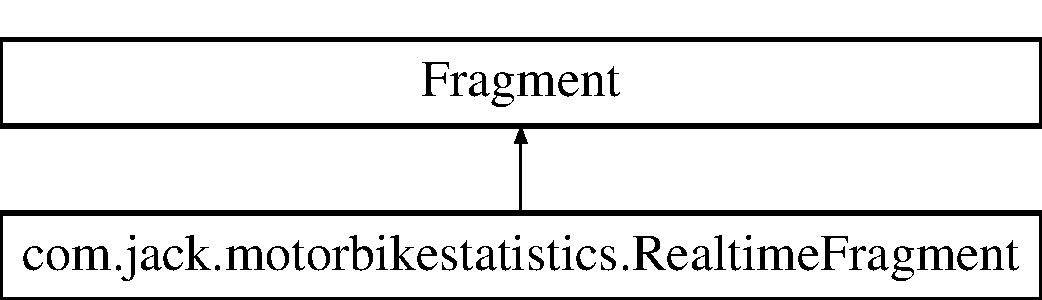
\includegraphics[height=2.000000cm]{classcom_1_1jack_1_1motorbikestatistics_1_1_realtime_fragment}
\end{center}
\end{figure}
\subsection*{Public Member Functions}
\begin{DoxyCompactItemize}
\item 
\mbox{\Hypertarget{classcom_1_1jack_1_1motorbikestatistics_1_1_realtime_fragment_a68850ca4bf4eabcdf4ed4005d5f0d4d7}\label{classcom_1_1jack_1_1motorbikestatistics_1_1_realtime_fragment_a68850ca4bf4eabcdf4ed4005d5f0d4d7}} 
View {\bfseries on\+Create\+View} (Layout\+Inflater inflater, View\+Group container, Bundle saved\+Instance\+State)
\end{DoxyCompactItemize}
\subsection*{Public Attributes}
\begin{DoxyCompactItemize}
\item 
final Handler {\bfseries R\+X\+Handler}
\end{DoxyCompactItemize}


\subsection{Detailed Description}
Created by Jack on 23-\/\+Jan-\/17. 

\subsection{Member Data Documentation}
\mbox{\Hypertarget{classcom_1_1jack_1_1motorbikestatistics_1_1_realtime_fragment_a7b39a40287200b7530c2d935e6717fa6}\label{classcom_1_1jack_1_1motorbikestatistics_1_1_realtime_fragment_a7b39a40287200b7530c2d935e6717fa6}} 
\index{com\+::jack\+::motorbikestatistics\+::\+Realtime\+Fragment@{com\+::jack\+::motorbikestatistics\+::\+Realtime\+Fragment}!R\+X\+Handler@{R\+X\+Handler}}
\index{R\+X\+Handler@{R\+X\+Handler}!com\+::jack\+::motorbikestatistics\+::\+Realtime\+Fragment@{com\+::jack\+::motorbikestatistics\+::\+Realtime\+Fragment}}
\subsubsection{\texorpdfstring{R\+X\+Handler}{RXHandler}}
{\footnotesize\ttfamily final Handler com.\+jack.\+motorbikestatistics.\+Realtime\+Fragment.\+R\+X\+Handler}

{\bfseries Initial value\+:}
\begin{DoxyCode}
= \textcolor{keyword}{new} Handler(Looper.getMainLooper()) \{

        @Override
        \textcolor{keyword}{public} \textcolor{keywordtype}{void} handleMessage(Message msg) \{

            Bundle msgData = msg.getData();
            String jsonString = msgData.getString(\textcolor{stringliteral}{"JSON"});

            \textcolor{keywordflow}{if} (jsonString != null) \{

                
                \textcolor{keywordflow}{try} \{
                    JSONObject tmpJSON = \textcolor{keyword}{new} JSONObject(jsonString);
                    newData(tmpJSON);

                \} \textcolor{keywordflow}{catch} (JSONException e) \{
                    
                \}
            \}
        \}
    \}
\end{DoxyCode}


The documentation for this class was generated from the following file\+:\begin{DoxyCompactItemize}
\item 
android-\/app/app/src/main/java/com/jack/motorbikestatistics/Realtime\+Fragment.\+java\end{DoxyCompactItemize}

\hypertarget{classcom_1_1jack_1_1motorbikestatistics_1_1_set_of_data_items}{}\section{com.\+jack.\+motorbikestatistics.\+Set\+Of\+Data\+Items Class Reference}
\label{classcom_1_1jack_1_1motorbikestatistics_1_1_set_of_data_items}\index{com.\+jack.\+motorbikestatistics.\+Set\+Of\+Data\+Items@{com.\+jack.\+motorbikestatistics.\+Set\+Of\+Data\+Items}}


Array\+List extension to allow searching via item name.  


Inheritance diagram for com.\+jack.\+motorbikestatistics.\+Set\+Of\+Data\+Items\+:\begin{figure}[H]
\begin{center}
\leavevmode
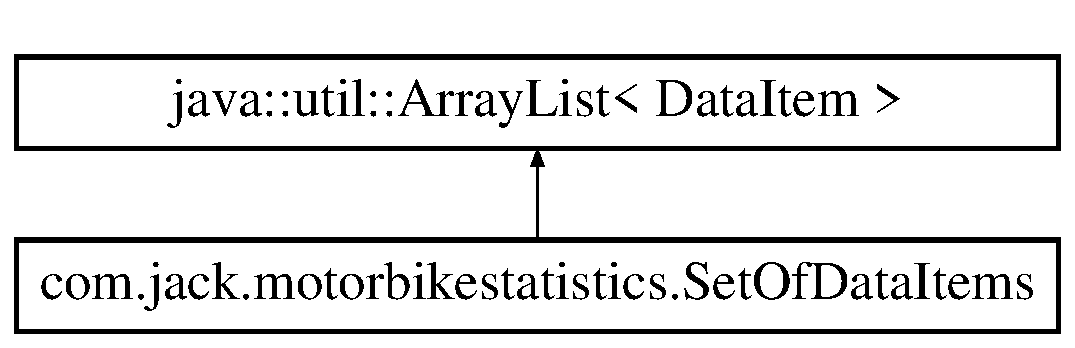
\includegraphics[height=2.000000cm]{classcom_1_1jack_1_1motorbikestatistics_1_1_set_of_data_items}
\end{center}
\end{figure}
\subsection*{Public Member Functions}
\begin{DoxyCompactItemize}
\item 
\mbox{\Hypertarget{classcom_1_1jack_1_1motorbikestatistics_1_1_set_of_data_items_adba096f9c8b7be1b32df7e6ef3f5e8ef}\label{classcom_1_1jack_1_1motorbikestatistics_1_1_set_of_data_items_adba096f9c8b7be1b32df7e6ef3f5e8ef}} 
\hyperlink{classcom_1_1jack_1_1motorbikestatistics_1_1_set_of_data_items_adba096f9c8b7be1b32df7e6ef3f5e8ef}{Set\+Of\+Data\+Items} ()
\begin{DoxyCompactList}\small\item\em Constructor, just calls inhereted constructor method. \end{DoxyCompactList}\item 
\hyperlink{classcom_1_1jack_1_1motorbikestatistics_1_1_data_item}{Data\+Item} \hyperlink{classcom_1_1jack_1_1motorbikestatistics_1_1_set_of_data_items_a028fb1f4ce3fd7991d73d368720c19d9}{get\+Item\+By\+Name} (String name)
\begin{DoxyCompactList}\small\item\em Function to allow searching of Array\+List$<$\+Data\+Item$>$ via name. \end{DoxyCompactList}\end{DoxyCompactItemize}


\subsection{Detailed Description}
Array\+List extension to allow searching via item name. 

\subsection{Member Function Documentation}
\mbox{\Hypertarget{classcom_1_1jack_1_1motorbikestatistics_1_1_set_of_data_items_a028fb1f4ce3fd7991d73d368720c19d9}\label{classcom_1_1jack_1_1motorbikestatistics_1_1_set_of_data_items_a028fb1f4ce3fd7991d73d368720c19d9}} 
\index{com\+::jack\+::motorbikestatistics\+::\+Set\+Of\+Data\+Items@{com\+::jack\+::motorbikestatistics\+::\+Set\+Of\+Data\+Items}!get\+Item\+By\+Name@{get\+Item\+By\+Name}}
\index{get\+Item\+By\+Name@{get\+Item\+By\+Name}!com\+::jack\+::motorbikestatistics\+::\+Set\+Of\+Data\+Items@{com\+::jack\+::motorbikestatistics\+::\+Set\+Of\+Data\+Items}}
\subsubsection{\texorpdfstring{get\+Item\+By\+Name()}{getItemByName()}}
{\footnotesize\ttfamily \hyperlink{classcom_1_1jack_1_1motorbikestatistics_1_1_data_item}{Data\+Item} com.\+jack.\+motorbikestatistics.\+Set\+Of\+Data\+Items.\+get\+Item\+By\+Name (\begin{DoxyParamCaption}\item[{String}]{name }\end{DoxyParamCaption})\hspace{0.3cm}{\ttfamily [inline]}}



Function to allow searching of Array\+List$<$\+Data\+Item$>$ via name. 

Loops through all items in array until one item with matching name is found. This is then returned by the function.


\begin{DoxyParams}{Parameters}
{\em name} & -\/ Name to match. \\
\hline
\end{DoxyParams}
\begin{DoxyReturn}{Returns}
\hyperlink{classcom_1_1jack_1_1motorbikestatistics_1_1_data_item}{Data\+Item} -\/ The item with matching name. 
\end{DoxyReturn}


References com.\+jack.\+motorbikestatistics.\+Data\+Item$<$ T $>$.\+get\+Name().


\begin{DoxyCode}
36                                                \{
37         DataItem result = null;
38 
39         \textcolor{keywordflow}{for} (DataItem item: \textcolor{keyword}{this}) \{
40             \textcolor{keywordflow}{if} (item.getName().equals(name)) \{
41                 result = item;
42                 \textcolor{keywordflow}{break};
43             \}
44         \}
45 
46         \textcolor{keywordflow}{return} result;
47     \}
\end{DoxyCode}


The documentation for this class was generated from the following file\+:\begin{DoxyCompactItemize}
\item 
android-\/app/app/src/main/java/com/jack/motorbikestatistics/\hyperlink{_set_of_data_items_8java}{Set\+Of\+Data\+Items.\+java}\end{DoxyCompactItemize}

\hypertarget{class_storage}{}\section{Storage Class Reference}
\label{class_storage}\index{Storage@{Storage}}
\subsection*{Public Member Functions}
\begin{DoxyCompactItemize}
\item 
\mbox{\Hypertarget{class_storage_a98b01eb20a64a4bf4127685147f7f6f1}\label{class_storage_a98b01eb20a64a4bf4127685147f7f6f1}} 
void {\bfseries init} ()
\item 
\mbox{\Hypertarget{class_storage_a044a17325b2917afca49aa19ddb488f6}\label{class_storage_a044a17325b2917afca49aa19ddb488f6}} 
bool {\bfseries save\+To\+File} (char data\mbox{[}$\,$\mbox{]}, bool new\+Line)
\item 
\mbox{\Hypertarget{class_storage_a571ce9630665d9407ffbaeff55c47b0a}\label{class_storage_a571ce9630665d9407ffbaeff55c47b0a}} 
bool {\bfseries generate\+File\+Name} ()
\item 
\mbox{\Hypertarget{class_storage_a4831b2e8ecfa22da6971f5a8690cc4e3}\label{class_storage_a4831b2e8ecfa22da6971f5a8690cc4e3}} 
void {\bfseries load\+Trip\+Names} ()
\item 
\mbox{\Hypertarget{class_storage_af56ca8289ed925300e3385114c561eec}\label{class_storage_af56ca8289ed925300e3385114c561eec}} 
void {\bfseries load\+Saved\+Trip} ()
\end{DoxyCompactItemize}


The documentation for this class was generated from the following files\+:\begin{DoxyCompactItemize}
\item 
logging-\/device/Storage.\+h\item 
logging-\/device/Storage.\+cpp\end{DoxyCompactItemize}

\hypertarget{classcom_1_1jack_1_1motorbikestatistics_1_1_trip_item}{}\section{com.\+jack.\+motorbikestatistics.\+Trip\+Item Class Reference}
\label{classcom_1_1jack_1_1motorbikestatistics_1_1_trip_item}\index{com.\+jack.\+motorbikestatistics.\+Trip\+Item@{com.\+jack.\+motorbikestatistics.\+Trip\+Item}}


Class used for holding name and size information relating to a trip.  


\subsection*{Public Member Functions}
\begin{DoxyCompactItemize}
\item 
\hyperlink{classcom_1_1jack_1_1motorbikestatistics_1_1_trip_item_a17a6df81af0062b7bf03babb4c7433b0}{Trip\+Item} (String name, int size)
\begin{DoxyCompactList}\small\item\em Constructor for creating of a \hyperlink{classcom_1_1jack_1_1motorbikestatistics_1_1_trip_item}{Trip\+Item}. \end{DoxyCompactList}\item 
String \hyperlink{classcom_1_1jack_1_1motorbikestatistics_1_1_trip_item_a0416f27a3fcd2344fca453f7a2a6b4d0}{get\+Trip\+Name} ()
\begin{DoxyCompactList}\small\item\em Getter for trip name. \end{DoxyCompactList}\item 
void \hyperlink{classcom_1_1jack_1_1motorbikestatistics_1_1_trip_item_a359fbbbde7fde3af75379054c87cfb2d}{set\+Trip\+Name} (String \hyperlink{classcom_1_1jack_1_1motorbikestatistics_1_1_trip_item_a2e678c328ae2972516c2da9d21826359}{trip\+Name})
\begin{DoxyCompactList}\small\item\em Setter for trip name. \end{DoxyCompactList}\item 
int \hyperlink{classcom_1_1jack_1_1motorbikestatistics_1_1_trip_item_aec0e07444e68e4492daa734bf3d6e24a}{get\+File\+Size} ()
\begin{DoxyCompactList}\small\item\em Getter for trip filesize. \end{DoxyCompactList}\item 
void \hyperlink{classcom_1_1jack_1_1motorbikestatistics_1_1_trip_item_a133ad3b07e6c5d57203ffdc81f6a51fc}{set\+File\+Size} (int \hyperlink{classcom_1_1jack_1_1motorbikestatistics_1_1_trip_item_ac7b1106a5db61eb17cfd3f314a885a3d}{file\+Size})
\begin{DoxyCompactList}\small\item\em Setter for trip filesize. \end{DoxyCompactList}\end{DoxyCompactItemize}
\subsection*{Private Attributes}
\begin{DoxyCompactItemize}
\item 
\mbox{\Hypertarget{classcom_1_1jack_1_1motorbikestatistics_1_1_trip_item_a2e678c328ae2972516c2da9d21826359}\label{classcom_1_1jack_1_1motorbikestatistics_1_1_trip_item_a2e678c328ae2972516c2da9d21826359}} 
String \hyperlink{classcom_1_1jack_1_1motorbikestatistics_1_1_trip_item_a2e678c328ae2972516c2da9d21826359}{trip\+Name} = null
\begin{DoxyCompactList}\small\item\em The trips name on the u\+SD card. \end{DoxyCompactList}\item 
\mbox{\Hypertarget{classcom_1_1jack_1_1motorbikestatistics_1_1_trip_item_ac7b1106a5db61eb17cfd3f314a885a3d}\label{classcom_1_1jack_1_1motorbikestatistics_1_1_trip_item_ac7b1106a5db61eb17cfd3f314a885a3d}} 
int \hyperlink{classcom_1_1jack_1_1motorbikestatistics_1_1_trip_item_ac7b1106a5db61eb17cfd3f314a885a3d}{file\+Size} = 0
\begin{DoxyCompactList}\small\item\em The trips file size on the u\+SD card. \end{DoxyCompactList}\end{DoxyCompactItemize}


\subsection{Detailed Description}
Class used for holding name and size information relating to a trip. 

\subsection{Constructor \& Destructor Documentation}
\mbox{\Hypertarget{classcom_1_1jack_1_1motorbikestatistics_1_1_trip_item_a17a6df81af0062b7bf03babb4c7433b0}\label{classcom_1_1jack_1_1motorbikestatistics_1_1_trip_item_a17a6df81af0062b7bf03babb4c7433b0}} 
\index{com\+::jack\+::motorbikestatistics\+::\+Trip\+Item@{com\+::jack\+::motorbikestatistics\+::\+Trip\+Item}!Trip\+Item@{Trip\+Item}}
\index{Trip\+Item@{Trip\+Item}!com\+::jack\+::motorbikestatistics\+::\+Trip\+Item@{com\+::jack\+::motorbikestatistics\+::\+Trip\+Item}}
\subsubsection{\texorpdfstring{Trip\+Item()}{TripItem()}}
{\footnotesize\ttfamily com.\+jack.\+motorbikestatistics.\+Trip\+Item.\+Trip\+Item (\begin{DoxyParamCaption}\item[{String}]{name,  }\item[{int}]{size }\end{DoxyParamCaption})\hspace{0.3cm}{\ttfamily [inline]}}



Constructor for creating of a \hyperlink{classcom_1_1jack_1_1motorbikestatistics_1_1_trip_item}{Trip\+Item}. 

Sets the original file name and size.


\begin{DoxyParams}{Parameters}
{\em name} & -\/ Trip name. \\
\hline
{\em size} & -\/ Size of the file. \\
\hline
\end{DoxyParams}

\begin{DoxyCode}
31                                            \{
32         this.\hyperlink{classcom_1_1jack_1_1motorbikestatistics_1_1_trip_item_a2e678c328ae2972516c2da9d21826359}{tripName} = name;
33         this.\hyperlink{classcom_1_1jack_1_1motorbikestatistics_1_1_trip_item_ac7b1106a5db61eb17cfd3f314a885a3d}{fileSize} = size;
34     \}
\end{DoxyCode}


\subsection{Member Function Documentation}
\mbox{\Hypertarget{classcom_1_1jack_1_1motorbikestatistics_1_1_trip_item_a0416f27a3fcd2344fca453f7a2a6b4d0}\label{classcom_1_1jack_1_1motorbikestatistics_1_1_trip_item_a0416f27a3fcd2344fca453f7a2a6b4d0}} 
\index{com\+::jack\+::motorbikestatistics\+::\+Trip\+Item@{com\+::jack\+::motorbikestatistics\+::\+Trip\+Item}!get\+Trip\+Name@{get\+Trip\+Name}}
\index{get\+Trip\+Name@{get\+Trip\+Name}!com\+::jack\+::motorbikestatistics\+::\+Trip\+Item@{com\+::jack\+::motorbikestatistics\+::\+Trip\+Item}}
\subsubsection{\texorpdfstring{get\+Trip\+Name()}{getTripName()}}
{\footnotesize\ttfamily String com.\+jack.\+motorbikestatistics.\+Trip\+Item.\+get\+Trip\+Name (\begin{DoxyParamCaption}{ }\end{DoxyParamCaption})\hspace{0.3cm}{\ttfamily [inline]}}



Getter for trip name. 

\begin{DoxyReturn}{Returns}
String -\/ Trip name. 
\end{DoxyReturn}


References com.\+jack.\+motorbikestatistics.\+Trip\+Item.\+trip\+Name.


\begin{DoxyCode}
40                                 \{
41         \textcolor{keywordflow}{return} \hyperlink{classcom_1_1jack_1_1motorbikestatistics_1_1_trip_item_a2e678c328ae2972516c2da9d21826359}{tripName};
42     \}
\end{DoxyCode}
\mbox{\Hypertarget{classcom_1_1jack_1_1motorbikestatistics_1_1_trip_item_a359fbbbde7fde3af75379054c87cfb2d}\label{classcom_1_1jack_1_1motorbikestatistics_1_1_trip_item_a359fbbbde7fde3af75379054c87cfb2d}} 
\index{com\+::jack\+::motorbikestatistics\+::\+Trip\+Item@{com\+::jack\+::motorbikestatistics\+::\+Trip\+Item}!set\+Trip\+Name@{set\+Trip\+Name}}
\index{set\+Trip\+Name@{set\+Trip\+Name}!com\+::jack\+::motorbikestatistics\+::\+Trip\+Item@{com\+::jack\+::motorbikestatistics\+::\+Trip\+Item}}
\subsubsection{\texorpdfstring{set\+Trip\+Name()}{setTripName()}}
{\footnotesize\ttfamily void com.\+jack.\+motorbikestatistics.\+Trip\+Item.\+set\+Trip\+Name (\begin{DoxyParamCaption}\item[{String}]{trip\+Name }\end{DoxyParamCaption})\hspace{0.3cm}{\ttfamily [inline]}}



Setter for trip name. 


\begin{DoxyParams}{Parameters}
{\em trip\+Name} & -\/ New trip name. \\
\hline
\end{DoxyParams}


References com.\+jack.\+motorbikestatistics.\+Trip\+Item.\+trip\+Name.


\begin{DoxyCode}
48                                              \{
49         this.\hyperlink{classcom_1_1jack_1_1motorbikestatistics_1_1_trip_item_a2e678c328ae2972516c2da9d21826359}{tripName} = \hyperlink{classcom_1_1jack_1_1motorbikestatistics_1_1_trip_item_a2e678c328ae2972516c2da9d21826359}{tripName};
50     \}
\end{DoxyCode}
\mbox{\Hypertarget{classcom_1_1jack_1_1motorbikestatistics_1_1_trip_item_aec0e07444e68e4492daa734bf3d6e24a}\label{classcom_1_1jack_1_1motorbikestatistics_1_1_trip_item_aec0e07444e68e4492daa734bf3d6e24a}} 
\index{com\+::jack\+::motorbikestatistics\+::\+Trip\+Item@{com\+::jack\+::motorbikestatistics\+::\+Trip\+Item}!get\+File\+Size@{get\+File\+Size}}
\index{get\+File\+Size@{get\+File\+Size}!com\+::jack\+::motorbikestatistics\+::\+Trip\+Item@{com\+::jack\+::motorbikestatistics\+::\+Trip\+Item}}
\subsubsection{\texorpdfstring{get\+File\+Size()}{getFileSize()}}
{\footnotesize\ttfamily int com.\+jack.\+motorbikestatistics.\+Trip\+Item.\+get\+File\+Size (\begin{DoxyParamCaption}{ }\end{DoxyParamCaption})\hspace{0.3cm}{\ttfamily [inline]}}



Getter for trip filesize. 

\begin{DoxyReturn}{Returns}
int -\/ Filesize in bytes. 
\end{DoxyReturn}


References com.\+jack.\+motorbikestatistics.\+Trip\+Item.\+file\+Size.


\begin{DoxyCode}
56                              \{
57         \textcolor{keywordflow}{return} \hyperlink{classcom_1_1jack_1_1motorbikestatistics_1_1_trip_item_ac7b1106a5db61eb17cfd3f314a885a3d}{fileSize};
58     \}
\end{DoxyCode}
\mbox{\Hypertarget{classcom_1_1jack_1_1motorbikestatistics_1_1_trip_item_a133ad3b07e6c5d57203ffdc81f6a51fc}\label{classcom_1_1jack_1_1motorbikestatistics_1_1_trip_item_a133ad3b07e6c5d57203ffdc81f6a51fc}} 
\index{com\+::jack\+::motorbikestatistics\+::\+Trip\+Item@{com\+::jack\+::motorbikestatistics\+::\+Trip\+Item}!set\+File\+Size@{set\+File\+Size}}
\index{set\+File\+Size@{set\+File\+Size}!com\+::jack\+::motorbikestatistics\+::\+Trip\+Item@{com\+::jack\+::motorbikestatistics\+::\+Trip\+Item}}
\subsubsection{\texorpdfstring{set\+File\+Size()}{setFileSize()}}
{\footnotesize\ttfamily void com.\+jack.\+motorbikestatistics.\+Trip\+Item.\+set\+File\+Size (\begin{DoxyParamCaption}\item[{int}]{file\+Size }\end{DoxyParamCaption})\hspace{0.3cm}{\ttfamily [inline]}}



Setter for trip filesize. 


\begin{DoxyParams}{Parameters}
{\em file\+Size} & -\/ New trip filesize. \\
\hline
\end{DoxyParams}


References com.\+jack.\+motorbikestatistics.\+Trip\+Item.\+file\+Size.


\begin{DoxyCode}
64                                           \{
65         this.\hyperlink{classcom_1_1jack_1_1motorbikestatistics_1_1_trip_item_ac7b1106a5db61eb17cfd3f314a885a3d}{fileSize} = \hyperlink{classcom_1_1jack_1_1motorbikestatistics_1_1_trip_item_ac7b1106a5db61eb17cfd3f314a885a3d}{fileSize};
66     \}
\end{DoxyCode}


The documentation for this class was generated from the following file\+:\begin{DoxyCompactItemize}
\item 
android-\/app/app/src/main/java/com/jack/motorbikestatistics/\hyperlink{_trip_item_8java}{Trip\+Item.\+java}\end{DoxyCompactItemize}

\hypertarget{classcom_1_1jack_1_1motorbikestatistics_1_1_trip_list_adapter}{}\section{com.\+jack.\+motorbikestatistics.\+Trip\+List\+Adapter Class Reference}
\label{classcom_1_1jack_1_1motorbikestatistics_1_1_trip_list_adapter}\index{com.\+jack.\+motorbikestatistics.\+Trip\+List\+Adapter@{com.\+jack.\+motorbikestatistics.\+Trip\+List\+Adapter}}
Inheritance diagram for com.\+jack.\+motorbikestatistics.\+Trip\+List\+Adapter\+:\begin{figure}[H]
\begin{center}
\leavevmode
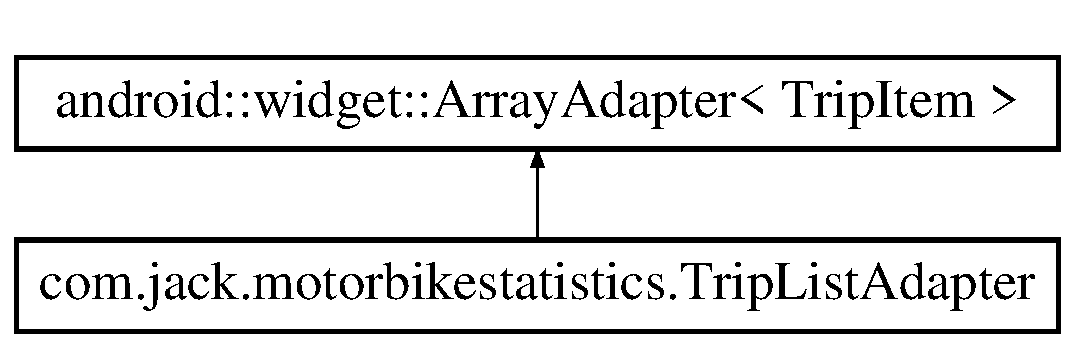
\includegraphics[height=2.000000cm]{classcom_1_1jack_1_1motorbikestatistics_1_1_trip_list_adapter}
\end{center}
\end{figure}
\subsection*{Public Member Functions}
\begin{DoxyCompactItemize}
\item 
\mbox{\Hypertarget{classcom_1_1jack_1_1motorbikestatistics_1_1_trip_list_adapter_ace5ca232bac9a2a6e0d1b61e88b35546}\label{classcom_1_1jack_1_1motorbikestatistics_1_1_trip_list_adapter_ace5ca232bac9a2a6e0d1b61e88b35546}} 
{\bfseries Trip\+List\+Adapter} (Context cnt, int layout\+Resource\+Id, Array\+List$<$ \hyperlink{classcom_1_1jack_1_1motorbikestatistics_1_1_trip_item}{Trip\+Item} $>$ data)
\item 
\mbox{\Hypertarget{classcom_1_1jack_1_1motorbikestatistics_1_1_trip_list_adapter_a1cfdc3feff28941d18e70ce0979d959d}\label{classcom_1_1jack_1_1motorbikestatistics_1_1_trip_list_adapter_a1cfdc3feff28941d18e70ce0979d959d}} 
View {\bfseries get\+View} (int position, View convert\+View, View\+Group parent)
\end{DoxyCompactItemize}


\subsection{Detailed Description}
Created by Jack on 26-\/\+Mar-\/17. 

The documentation for this class was generated from the following file\+:\begin{DoxyCompactItemize}
\item 
android-\/app/app/src/main/java/com/jack/motorbikestatistics/Trip\+List\+Adapter.\+java\end{DoxyCompactItemize}

\hypertarget{classcom_1_1jack_1_1motorbikestatistics_1_1_data_list_adapter_1_1_view_holder}{}\section{com.\+jack.\+motorbikestatistics.\+Data\+List\+Adapter.\+View\+Holder Class Reference}
\label{classcom_1_1jack_1_1motorbikestatistics_1_1_data_list_adapter_1_1_view_holder}\index{com.\+jack.\+motorbikestatistics.\+Data\+List\+Adapter.\+View\+Holder@{com.\+jack.\+motorbikestatistics.\+Data\+List\+Adapter.\+View\+Holder}}


The documentation for this class was generated from the following file\+:\begin{DoxyCompactItemize}
\item 
android-\/app/app/src/main/java/com/jack/motorbikestatistics/Data\+List\+Adapter.\+java\end{DoxyCompactItemize}

\hypertarget{classcom_1_1jack_1_1motorbikestatistics_1_1_b_t_device_list_adapter_1_1_view_holder}{}\section{com.\+jack.\+motorbikestatistics.\+B\+T\+Device\+List\+Adapter.\+View\+Holder Class Reference}
\label{classcom_1_1jack_1_1motorbikestatistics_1_1_b_t_device_list_adapter_1_1_view_holder}\index{com.\+jack.\+motorbikestatistics.\+B\+T\+Device\+List\+Adapter.\+View\+Holder@{com.\+jack.\+motorbikestatistics.\+B\+T\+Device\+List\+Adapter.\+View\+Holder}}


The documentation for this class was generated from the following file\+:\begin{DoxyCompactItemize}
\item 
android-\/app/app/src/main/java/com/jack/motorbikestatistics/B\+T\+Device\+List\+Adapter.\+java\end{DoxyCompactItemize}

\hypertarget{classcom_1_1jack_1_1motorbikestatistics_1_1_trip_list_adapter_1_1_view_holder}{}\section{com.\+jack.\+motorbikestatistics.\+Trip\+List\+Adapter.\+View\+Holder Class Reference}
\label{classcom_1_1jack_1_1motorbikestatistics_1_1_trip_list_adapter_1_1_view_holder}\index{com.\+jack.\+motorbikestatistics.\+Trip\+List\+Adapter.\+View\+Holder@{com.\+jack.\+motorbikestatistics.\+Trip\+List\+Adapter.\+View\+Holder}}


The documentation for this class was generated from the following file\+:\begin{DoxyCompactItemize}
\item 
android-\/app/app/src/main/java/com/jack/motorbikestatistics/Trip\+List\+Adapter.\+java\end{DoxyCompactItemize}

\chapter{File Documentation}
\hypertarget{_b_t_connection_8java}{}\section{android-\/app/app/src/main/java/com/jack/motorbikestatistics/\+B\+T\+Connection.java File Reference}
\label{_b_t_connection_8java}\index{android-\/app/app/src/main/java/com/jack/motorbikestatistics/\+B\+T\+Connection.\+java@{android-\/app/app/src/main/java/com/jack/motorbikestatistics/\+B\+T\+Connection.\+java}}


Class for holding containing bluetooth connection on app.  


\subsection*{Classes}
\begin{DoxyCompactItemize}
\item 
class \hyperlink{classcom_1_1jack_1_1motorbikestatistics_1_1_b_t_connection}{com.\+jack.\+motorbikestatistics.\+B\+T\+Connection}
\end{DoxyCompactItemize}


\subsection{Detailed Description}
Class for holding containing bluetooth connection on app. 

Class runs in a seperate thread to main UI allowing for concurrent transmission and receiving of data to/from the logging device.

\begin{DoxyAuthor}{Author}
Jack Allister -\/ 23042098 
\end{DoxyAuthor}
\begin{DoxyDate}{Date}
2016-\/2017 
\end{DoxyDate}

\hypertarget{_b_t_device_item_8java}{}\section{android-\/app/app/src/main/java/com/jack/motorbikestatistics/\+B\+T\+Device\+Item.java File Reference}
\label{_b_t_device_item_8java}\index{android-\/app/app/src/main/java/com/jack/motorbikestatistics/\+B\+T\+Device\+Item.\+java@{android-\/app/app/src/main/java/com/jack/motorbikestatistics/\+B\+T\+Device\+Item.\+java}}


UI class for holding information regarding a bluetooth device.  


\subsection*{Classes}
\begin{DoxyCompactItemize}
\item 
class \hyperlink{class_android_app_1_1_b_t_device_item}{Android\+App.\+B\+T\+Device\+Item}
\begin{DoxyCompactList}\small\item\em Class used for holding core UI information of a bluetooth devices. \end{DoxyCompactList}\end{DoxyCompactItemize}


\subsection{Detailed Description}
UI class for holding information regarding a bluetooth device. 

Implemented for the List\+View that shows unpaired/paired \& connected bluetooth devices.

\begin{DoxyAuthor}{Author}
Jack Allister -\/ 23042098 
\end{DoxyAuthor}
\begin{DoxyDate}{Date}
2016-\/2017 
\end{DoxyDate}

\hypertarget{_b_t_device_list_adapter_8java}{}\section{android-\/app/app/src/main/java/com/jack/motorbikestatistics/\+B\+T\+Device\+List\+Adapter.java File Reference}
\label{_b_t_device_list_adapter_8java}\index{android-\/app/app/src/main/java/com/jack/motorbikestatistics/\+B\+T\+Device\+List\+Adapter.\+java@{android-\/app/app/src/main/java/com/jack/motorbikestatistics/\+B\+T\+Device\+List\+Adapter.\+java}}


UI List\+View adapter to display bluetooth devices.  


\subsection*{Classes}
\begin{DoxyCompactItemize}
\item 
class \hyperlink{classcom_1_1jack_1_1motorbikestatistics_1_1_b_t_device_list_adapter}{com.\+jack.\+motorbikestatistics.\+B\+T\+Device\+List\+Adapter}
\begin{DoxyCompactList}\small\item\em Adapter class used for displaying bluetooth devices. \end{DoxyCompactList}\item 
class \hyperlink{classcom_1_1jack_1_1motorbikestatistics_1_1_b_t_device_list_adapter_1_1_view_holder}{com.\+jack.\+motorbikestatistics.\+B\+T\+Device\+List\+Adapter.\+View\+Holder}
\begin{DoxyCompactList}\small\item\em Class that holds all data displayed for each List\+Item. \end{DoxyCompactList}\end{DoxyCompactItemize}


\subsection{Detailed Description}
UI List\+View adapter to display bluetooth devices. 

Implemented so that the device List\+View can display relevant information relating to the Bluetooth\+Device\textquotesingle{}s that are available to pair, connect.

\begin{DoxyAuthor}{Author}
Jack Allister -\/ 23042098 
\end{DoxyAuthor}
\begin{DoxyDate}{Date}
2016-\/2017 
\end{DoxyDate}

\hypertarget{_data_item_8java}{}\section{android-\/app/app/src/main/java/com/jack/motorbikestatistics/\+Data\+Item.java File Reference}
\label{_data_item_8java}\index{android-\/app/app/src/main/java/com/jack/motorbikestatistics/\+Data\+Item.\+java@{android-\/app/app/src/main/java/com/jack/motorbikestatistics/\+Data\+Item.\+java}}


UI class for holding information regarding a specific statistic.  


\subsection*{Classes}
\begin{DoxyCompactItemize}
\item 
class \hyperlink{classcom_1_1jack_1_1motorbikestatistics_1_1_data_item}{com.\+jack.\+motorbikestatistics.\+Data\+Item$<$ T $>$}
\begin{DoxyCompactList}\small\item\em Class used for holding and displaying a piece of data within the statistic List\+View UI. \end{DoxyCompactList}\end{DoxyCompactItemize}


\subsection{Detailed Description}
UI class for holding information regarding a specific statistic. 

Implementation of generic class to allow multiple data types android added functionality such as averaging, minimum and maximum.

\begin{DoxyAuthor}{Author}
Jack Allister -\/ 23042098 
\end{DoxyAuthor}
\begin{DoxyDate}{Date}
2016-\/2017 
\end{DoxyDate}

\hypertarget{_data_list_adapter_8java}{}\section{android-\/app/app/src/main/java/com/jack/motorbikestatistics/\+Data\+List\+Adapter.java File Reference}
\label{_data_list_adapter_8java}\index{android-\/app/app/src/main/java/com/jack/motorbikestatistics/\+Data\+List\+Adapter.\+java@{android-\/app/app/src/main/java/com/jack/motorbikestatistics/\+Data\+List\+Adapter.\+java}}


UI List\+View adapter to display statistics.  


\subsection*{Classes}
\begin{DoxyCompactItemize}
\item 
class \hyperlink{classcom_1_1jack_1_1motorbikestatistics_1_1_data_list_adapter}{com.\+jack.\+motorbikestatistics.\+Data\+List\+Adapter}
\begin{DoxyCompactList}\small\item\em Adapter class used for displaying statistics. \end{DoxyCompactList}\item 
class \hyperlink{classcom_1_1jack_1_1motorbikestatistics_1_1_data_list_adapter_1_1_view_holder}{com.\+jack.\+motorbikestatistics.\+Data\+List\+Adapter.\+View\+Holder}
\begin{DoxyCompactList}\small\item\em Class that holds all data displayed for each List\+Item. \end{DoxyCompactList}\end{DoxyCompactItemize}


\subsection{Detailed Description}
UI List\+View adapter to display statistics. 

Implemented so that the statistics List\+View can display relevant information relating to the statistic such as name, value, average, min \& max.

\begin{DoxyAuthor}{Author}
Jack Allister -\/ 23042098 
\end{DoxyAuthor}
\begin{DoxyDate}{Date}
2016-\/2017 
\end{DoxyDate}

\hypertarget{_load_device_fragment_8java}{}\section{android-\/app/app/src/main/java/com/jack/motorbikestatistics/\+Load\+Device\+Fragment.java File Reference}
\label{_load_device_fragment_8java}\index{android-\/app/app/src/main/java/com/jack/motorbikestatistics/\+Load\+Device\+Fragment.\+java@{android-\/app/app/src/main/java/com/jack/motorbikestatistics/\+Load\+Device\+Fragment.\+java}}


Fragment/\+Tab for providing UI for loading from device.  


\subsection*{Classes}
\begin{DoxyCompactItemize}
\item 
class \hyperlink{class_android_app_1_1_load_device_fragment}{Android\+App.\+Load\+Device\+Fragment}
\begin{DoxyCompactList}\small\item\em UI Class for loading saved trips from device. \end{DoxyCompactList}\item 
class \hyperlink{class_android_app_1_1_load_device_fragment_1_1_trip_item_listener}{Android\+App.\+Load\+Device\+Fragment.\+Trip\+Item\+Listener}
\begin{DoxyCompactList}\small\item\em Listener used to identify when a trip has been pressed. \end{DoxyCompactList}\end{DoxyCompactItemize}


\subsection{Detailed Description}
Fragment/\+Tab for providing UI for loading from device. 

UI to allow the user to load saved trips stored on the u\+SD of the logging device.

\begin{DoxyAuthor}{Author}
Jack Allister -\/ 23042098 
\end{DoxyAuthor}
\begin{DoxyDate}{Date}
2016-\/2017 
\end{DoxyDate}

\hypertarget{_main_activity_8java}{}\section{android-\/app/app/src/main/java/com/jack/motorbikestatistics/\+Main\+Activity.java File Reference}
\label{_main_activity_8java}\index{android-\/app/app/src/main/java/com/jack/motorbikestatistics/\+Main\+Activity.\+java@{android-\/app/app/src/main/java/com/jack/motorbikestatistics/\+Main\+Activity.\+java}}


Main activity class responsible for tabbing.  


\subsection*{Classes}
\begin{DoxyCompactItemize}
\item 
class \hyperlink{class_android_app_1_1_main_activity}{Android\+App.\+Main\+Activity}
\begin{DoxyCompactList}\small\item\em Main activity class for fragment navigation. \end{DoxyCompactList}\end{DoxyCompactItemize}


\subsection{Detailed Description}
Main activity class responsible for tabbing. 

Responsible for navigation between each fragment/tab. Sends relevant commands to switch system modes on the logging device as well.

\begin{DoxyAuthor}{Author}
Jack Allister -\/ 23042098 
\end{DoxyAuthor}
\begin{DoxyDate}{Date}
2016-\/2017 
\end{DoxyDate}

\hypertarget{_maps_activity_8java}{}\section{android-\/app/app/src/main/java/com/jack/motorbikestatistics/\+Maps\+Activity.java File Reference}
\label{_maps_activity_8java}\index{android-\/app/app/src/main/java/com/jack/motorbikestatistics/\+Maps\+Activity.\+java@{android-\/app/app/src/main/java/com/jack/motorbikestatistics/\+Maps\+Activity.\+java}}


Maps activity class reponsible for showing data on Google Maps.  


\subsection*{Classes}
\begin{DoxyCompactItemize}
\item 
class \hyperlink{classcom_1_1jack_1_1motorbikestatistics_1_1_maps_activity}{com.\+jack.\+motorbikestatistics.\+Maps\+Activity}
\begin{DoxyCompactList}\small\item\em Maps activity class for displaying map data. \end{DoxyCompactList}\end{DoxyCompactItemize}


\subsection{Detailed Description}
Maps activity class reponsible for showing data on Google Maps. 

Responsible for showing trip data on google maps. Places clickable points 5m away from each other showing stats at that point.

\begin{DoxyAuthor}{Author}
Jack Allister -\/ 23042098 
\end{DoxyAuthor}
\begin{DoxyDate}{Date}
2016-\/2017 
\end{DoxyDate}

\hypertarget{logging-device_8ino}{}\section{logging-\/device/logging-\/device.ino File Reference}
\label{logging-device_8ino}\index{logging-\/device/logging-\/device.\+ino@{logging-\/device/logging-\/device.\+ino}}


Arduino sketch for the logging device.  


{\ttfamily \#include $<$Software\+Serial.\+h$>$}\newline
{\ttfamily \#include $<$Tiny\+G\+P\+S++.\+h$>$}\newline
{\ttfamily \#include $<$Arduino\+Json.\+h$>$}\newline
{\ttfamily \#include \char`\"{}Orientation.\+h\char`\"{}}\newline
{\ttfamily \#include \char`\"{}Storage.\+h\char`\"{}}\newline
\subsection*{Macros}
\begin{DoxyCompactItemize}
\item 
\mbox{\Hypertarget{logging-device_8ino_ad7f0721d7856c100a69be7fa82e2865b}\label{logging-device_8ino_ad7f0721d7856c100a69be7fa82e2865b}} 
\#define \hyperlink{logging-device_8ino_ad7f0721d7856c100a69be7fa82e2865b}{I\+D\+L\+E\+\_\+\+C\+H\+AR}~\textquotesingle{}0\textquotesingle{}
\begin{DoxyCompactList}\small\item\em Command to set system to idle mode. \end{DoxyCompactList}\item 
\mbox{\Hypertarget{logging-device_8ino_a911a5839eebf5e3d5927f4f77e9bfb62}\label{logging-device_8ino_a911a5839eebf5e3d5927f4f77e9bfb62}} 
\#define \hyperlink{logging-device_8ino_a911a5839eebf5e3d5927f4f77e9bfb62}{R\+E\+A\+L\+T\+I\+M\+E\+\_\+\+C\+H\+AR}~\textquotesingle{}1\textquotesingle{}
\begin{DoxyCompactList}\small\item\em Command to set system to realtime logging mode. \end{DoxyCompactList}\item 
\mbox{\Hypertarget{logging-device_8ino_a4ffb22b7b0017657087830d24f68a323}\label{logging-device_8ino_a4ffb22b7b0017657087830d24f68a323}} 
\#define \hyperlink{logging-device_8ino_a4ffb22b7b0017657087830d24f68a323}{L\+I\+S\+T\+\_\+\+S\+A\+V\+E\+D\+\_\+\+C\+H\+AR}~\textquotesingle{}2\textquotesingle{}
\begin{DoxyCompactList}\small\item\em Command to list all saved trip names from u\+SD. \end{DoxyCompactList}\item 
\mbox{\Hypertarget{logging-device_8ino_aa72e33a6bcfedf9118f573741b4e137b}\label{logging-device_8ino_aa72e33a6bcfedf9118f573741b4e137b}} 
\#define \hyperlink{logging-device_8ino_aa72e33a6bcfedf9118f573741b4e137b}{L\+O\+A\+D\+\_\+\+T\+R\+I\+P\+\_\+\+C\+H\+AR}~\textquotesingle{}3\textquotesingle{}
\begin{DoxyCompactList}\small\item\em Command to load a trip stored on u\+SD. \end{DoxyCompactList}\item 
\mbox{\Hypertarget{logging-device_8ino_ad1e6e6f6fc813b305067b9e1b0777ea6}\label{logging-device_8ino_ad1e6e6f6fc813b305067b9e1b0777ea6}} 
\#define \hyperlink{logging-device_8ino_ad1e6e6f6fc813b305067b9e1b0777ea6}{B\+T\+\_\+\+S\+E\+R\+I\+AL}~Serial1
\begin{DoxyCompactList}\small\item\em Mapping for which H\+W-\/\+Serial port BT module is on. \end{DoxyCompactList}\item 
\mbox{\Hypertarget{logging-device_8ino_a6882992121626898bccaa43be51ba4c2}\label{logging-device_8ino_a6882992121626898bccaa43be51ba4c2}} 
\#define \hyperlink{logging-device_8ino_a6882992121626898bccaa43be51ba4c2}{B\+T\+\_\+\+B\+A\+UD}~115200
\begin{DoxyCompactList}\small\item\em B\+A\+UD rate of BT device. \end{DoxyCompactList}\item 
\mbox{\Hypertarget{logging-device_8ino_acae14b9c1767cfec367a4b96009c94e5}\label{logging-device_8ino_acae14b9c1767cfec367a4b96009c94e5}} 
\#define \hyperlink{logging-device_8ino_acae14b9c1767cfec367a4b96009c94e5}{G\+P\+S\+\_\+\+T\+X\+\_\+\+P\+IN}~9
\begin{DoxyCompactList}\small\item\em G\+PS serial transmit pin. \end{DoxyCompactList}\item 
\mbox{\Hypertarget{logging-device_8ino_a6f8927970de9eedcbb8f6c14b1d0d6c3}\label{logging-device_8ino_a6f8927970de9eedcbb8f6c14b1d0d6c3}} 
\#define \hyperlink{logging-device_8ino_a6f8927970de9eedcbb8f6c14b1d0d6c3}{G\+P\+S\+\_\+\+R\+X\+\_\+\+P\+IN}~8
\begin{DoxyCompactList}\small\item\em G\+PS serial receive pin. \end{DoxyCompactList}\item 
\mbox{\Hypertarget{logging-device_8ino_af0875ffe69dbe45df3f85c1f720c3eee}\label{logging-device_8ino_af0875ffe69dbe45df3f85c1f720c3eee}} 
\#define \hyperlink{logging-device_8ino_af0875ffe69dbe45df3f85c1f720c3eee}{G\+P\+S\+\_\+\+B\+A\+UD}~9600
\begin{DoxyCompactList}\small\item\em G\+PS serial baud rate. \end{DoxyCompactList}\item 
\mbox{\Hypertarget{logging-device_8ino_ab4553be4db9860d940f81d7447173b2f}\label{logging-device_8ino_ab4553be4db9860d940f81d7447173b2f}} 
\#define \hyperlink{logging-device_8ino_ab4553be4db9860d940f81d7447173b2f}{L\+E\+D\+\_\+\+P\+IN}~13
\begin{DoxyCompactList}\small\item\em L\+ED pin to indicate read. \end{DoxyCompactList}\end{DoxyCompactItemize}
\subsection*{Enumerations}
\begin{DoxyCompactItemize}
\item 
\mbox{\Hypertarget{logging-device_8ino_a980e950615d86dadef54f3cfaefb5fb4}\label{logging-device_8ino_a980e950615d86dadef54f3cfaefb5fb4}} 
enum \hyperlink{logging-device_8ino_a980e950615d86dadef54f3cfaefb5fb4}{O\+P\+E\+R\+A\+T\+I\+N\+G\+\_\+\+M\+O\+DE} \{ {\bfseries I\+D\+LE}, 
{\bfseries R\+E\+A\+L\+T\+I\+ME}
 \}\begin{DoxyCompactList}\small\item\em Typedef holding two possible states for device. \end{DoxyCompactList}
\end{DoxyCompactItemize}
\subsection*{Functions}
\begin{DoxyCompactItemize}
\item 
\mbox{\Hypertarget{logging-device_8ino_aa2475f51bdc0f31d16d2916991d618d9}\label{logging-device_8ino_aa2475f51bdc0f31d16d2916991d618d9}} 
Software\+Serial \hyperlink{logging-device_8ino_aa2475f51bdc0f31d16d2916991d618d9}{ser\+G\+PS} (\hyperlink{logging-device_8ino_a6f8927970de9eedcbb8f6c14b1d0d6c3}{G\+P\+S\+\_\+\+R\+X\+\_\+\+P\+IN}, \hyperlink{logging-device_8ino_acae14b9c1767cfec367a4b96009c94e5}{G\+P\+S\+\_\+\+T\+X\+\_\+\+P\+IN})
\begin{DoxyCompactList}\small\item\em Serial object for communicating with G\+PS module. \end{DoxyCompactList}\item 
void \hyperlink{logging-device_8ino_a4fc01d736fe50cf5b977f755b675f11d}{setup} ()
\begin{DoxyCompactList}\small\item\em Runs once at boot of arduino. \end{DoxyCompactList}\item 
void \hyperlink{logging-device_8ino_afe461d27b9c48d5921c00d521181f12f}{loop} ()
\begin{DoxyCompactList}\small\item\em Main system loop for arduino. \end{DoxyCompactList}\item 
bool \hyperlink{logging-device_8ino_aec1eb39e3cfde6331c4d29938c952c84}{parse\+New\+Mode} (char mode\+Char, \hyperlink{logging-device_8ino_a980e950615d86dadef54f3cfaefb5fb4}{O\+P\+E\+R\+A\+T\+I\+N\+G\+\_\+\+M\+O\+DE} \&new\+Mode)
\begin{DoxyCompactList}\small\item\em Returns whether system should change operating mode. \end{DoxyCompactList}\item 
void \hyperlink{logging-device_8ino_ab4c1c4c0fa047e336f9f4176406a54f1}{real\+Time\+Mode} ()
\begin{DoxyCompactList}\small\item\em Responsible for completing work needed in relatime mode. \end{DoxyCompactList}\item 
void \hyperlink{logging-device_8ino_a8d3614b16b26b9734d79e9f8f6695af3}{add\+Orientation\+To\+J\+S\+ON} ()
\begin{DoxyCompactList}\small\item\em Responsible for updating orientation J\+S\+ON object with newest information. \end{DoxyCompactList}\item 
void \hyperlink{logging-device_8ino_af1705fad6a6282b24379a174e18d4fe4}{add\+G\+P\+S\+To\+J\+S\+ON} ()
\begin{DoxyCompactList}\small\item\em Responsible for updating G\+PS J\+S\+ON object with newest information. \end{DoxyCompactList}\item 
void \hyperlink{logging-device_8ino_a9e4931f452cd25dfff67d41e7c9c0efb}{add\+Time\+To\+J\+S\+ON} ()
\begin{DoxyCompactList}\small\item\em Responsible for updating time J\+S\+ON object with newest information. \end{DoxyCompactList}\end{DoxyCompactItemize}
\subsection*{Variables}
\begin{DoxyCompactItemize}
\item 
\mbox{\Hypertarget{logging-device_8ino_a13a2ecbcf455940dd240e54e9e39cf7a}\label{logging-device_8ino_a13a2ecbcf455940dd240e54e9e39cf7a}} 
\hyperlink{logging-device_8ino_a980e950615d86dadef54f3cfaefb5fb4}{O\+P\+E\+R\+A\+T\+I\+N\+G\+\_\+\+M\+O\+DE} \hyperlink{logging-device_8ino_a13a2ecbcf455940dd240e54e9e39cf7a}{system\+Mode} = I\+D\+LE
\begin{DoxyCompactList}\small\item\em State machine for system state of device. \end{DoxyCompactList}\item 
\mbox{\Hypertarget{logging-device_8ino_a47be0262307aa023a1bda3d98986a16d}\label{logging-device_8ino_a47be0262307aa023a1bda3d98986a16d}} 
\hyperlink{class_orientation}{Orientation} \hyperlink{logging-device_8ino_a47be0262307aa023a1bda3d98986a16d}{orientation}
\begin{DoxyCompactList}\small\item\em \hyperlink{class_orientation}{Orientation} object, used for receiving device orientation. \end{DoxyCompactList}\item 
\mbox{\Hypertarget{logging-device_8ino_a40059244119c00baa1b841119cfd1b2e}\label{logging-device_8ino_a40059244119c00baa1b841119cfd1b2e}} 
\hyperlink{class_storage}{Storage} \hyperlink{logging-device_8ino_a40059244119c00baa1b841119cfd1b2e}{storage}
\begin{DoxyCompactList}\small\item\em \hyperlink{class_storage}{Storage} object, responsible for saving \& loading from u\+SD. \end{DoxyCompactList}\item 
\mbox{\Hypertarget{logging-device_8ino_a169c53997a7da1d0fb99aec1b4675ce8}\label{logging-device_8ino_a169c53997a7da1d0fb99aec1b4675ce8}} 
Tiny\+G\+P\+S\+Plus \hyperlink{logging-device_8ino_a169c53997a7da1d0fb99aec1b4675ce8}{gps}
\begin{DoxyCompactList}\small\item\em Our G\+PS object, responsible for parsing N\+M\+EA codes. \end{DoxyCompactList}\item 
\mbox{\Hypertarget{logging-device_8ino_ae3799d2cbf8f13e21cbaef64b75c6833}\label{logging-device_8ino_ae3799d2cbf8f13e21cbaef64b75c6833}} 
Static\+Json\+Buffer$<$ 500 $>$ \hyperlink{logging-device_8ino_ae3799d2cbf8f13e21cbaef64b75c6833}{json\+Buffer}
\begin{DoxyCompactList}\small\item\em Allocated space for holding all J\+S\+ON objects within. \end{DoxyCompactList}\item 
\mbox{\Hypertarget{logging-device_8ino_a5eebfb3b76a83174d0f5d032d1f6bfb7}\label{logging-device_8ino_a5eebfb3b76a83174d0f5d032d1f6bfb7}} 
Json\+Object \& \hyperlink{logging-device_8ino_a5eebfb3b76a83174d0f5d032d1f6bfb7}{main\+J\+S\+ON} = json\+Buffer.\+create\+Object()
\begin{DoxyCompactList}\small\item\em Parent J\+S\+ON object, holds orientation, time \& gps children. \end{DoxyCompactList}\item 
\mbox{\Hypertarget{logging-device_8ino_ae8e95a76df2aaa373792e5b744a6bb73}\label{logging-device_8ino_ae8e95a76df2aaa373792e5b744a6bb73}} 
Json\+Object \& \hyperlink{logging-device_8ino_ae8e95a76df2aaa373792e5b744a6bb73}{orient\+J\+S\+ON} = main\+J\+S\+O\+N.\+create\+Nested\+Object(\char`\"{}orientation\char`\"{})
\begin{DoxyCompactList}\small\item\em Holds all orientation related information. \end{DoxyCompactList}\item 
\mbox{\Hypertarget{logging-device_8ino_a548727e041a5cd3db91bdbd0ccd71e30}\label{logging-device_8ino_a548727e041a5cd3db91bdbd0ccd71e30}} 
Json\+Object \& \hyperlink{logging-device_8ino_a548727e041a5cd3db91bdbd0ccd71e30}{gps\+J\+S\+ON} = main\+J\+S\+O\+N.\+create\+Nested\+Object(\char`\"{}gps\char`\"{})
\begin{DoxyCompactList}\small\item\em Holds all location related information. \end{DoxyCompactList}\item 
\mbox{\Hypertarget{logging-device_8ino_acc172a29cb5ff709b48b650d9fb6503c}\label{logging-device_8ino_acc172a29cb5ff709b48b650d9fb6503c}} 
Json\+Object \& \hyperlink{logging-device_8ino_acc172a29cb5ff709b48b650d9fb6503c}{time\+J\+S\+ON} = main\+J\+S\+O\+N.\+create\+Nested\+Object(\char`\"{}time\char`\"{})
\begin{DoxyCompactList}\small\item\em Holds all time related inforamtion. \end{DoxyCompactList}\end{DoxyCompactItemize}


\subsection{Detailed Description}
Arduino sketch for the logging device. 

\begin{DoxyAuthor}{Author}
Jack Allister -\/ 23042098 
\end{DoxyAuthor}
\begin{DoxyDate}{Date}
2016-\/2017
\begin{DoxyItemize}
\item Arduino 101
\item Sparkfun G\+PS Logger shield
\item Onboard gyroscope + accelerometer
\item H\+C-\/06 Serial Bluetooth Module 
\end{DoxyItemize}
\end{DoxyDate}


\subsection{Function Documentation}
\mbox{\Hypertarget{logging-device_8ino_a4fc01d736fe50cf5b977f755b675f11d}\label{logging-device_8ino_a4fc01d736fe50cf5b977f755b675f11d}} 
\index{logging-\/device.\+ino@{logging-\/device.\+ino}!setup@{setup}}
\index{setup@{setup}!logging-\/device.\+ino@{logging-\/device.\+ino}}
\subsubsection{\texorpdfstring{setup()}{setup()}}
{\footnotesize\ttfamily void setup (\begin{DoxyParamCaption}{ }\end{DoxyParamCaption})}



Runs once at boot of arduino. 

Responsible for setting up the peripherals. ~\newline
Initialises modules such as storage, bluetooth \& gps. 

References B\+T\+\_\+\+B\+A\+UD, B\+T\+\_\+\+S\+E\+R\+I\+AL, G\+P\+S\+\_\+\+B\+A\+UD, L\+E\+D\+\_\+\+P\+IN, and ser\+G\+P\+S().


\begin{DoxyCode}
98 \{
99   pinMode(\hyperlink{logging-device_8ino_ab4553be4db9860d940f81d7447173b2f}{LED\_PIN}, OUTPUT);
100 
101   \textcolor{comment}{/* Initialise our storage module */}
102   \hyperlink{logging-device_8ino_a40059244119c00baa1b841119cfd1b2e}{storage}.init();
103 
104   \textcolor{comment}{/* Set up serial for data transmission */}
105   \hyperlink{logging-device_8ino_ad1e6e6f6fc813b305067b9e1b0777ea6}{BT\_SERIAL}.begin(\hyperlink{logging-device_8ino_a6882992121626898bccaa43be51ba4c2}{BT\_BAUD});
106 
107   \textcolor{comment}{/* Set up GPS */}
108   \hyperlink{logging-device_8ino_aa2475f51bdc0f31d16d2916991d618d9}{serGPS}.begin(\hyperlink{logging-device_8ino_af0875ffe69dbe45df3f85c1f720c3eee}{GPS\_BAUD});
109 \}
\end{DoxyCode}
\mbox{\Hypertarget{logging-device_8ino_afe461d27b9c48d5921c00d521181f12f}\label{logging-device_8ino_afe461d27b9c48d5921c00d521181f12f}} 
\index{logging-\/device.\+ino@{logging-\/device.\+ino}!loop@{loop}}
\index{loop@{loop}!logging-\/device.\+ino@{logging-\/device.\+ino}}
\subsubsection{\texorpdfstring{loop()}{loop()}}
{\footnotesize\ttfamily void loop (\begin{DoxyParamCaption}{ }\end{DoxyParamCaption})}



Main system loop for arduino. 

Checks serial to see if any commands are available. ~\newline
If available reads the byte and changes system mode relating to it. ~\newline
~\newline
System state machine is also iterated through each loop. ~\newline
Relevant procedure depending on system state is then called. 

References B\+T\+\_\+\+S\+E\+R\+I\+AL, parse\+New\+Mode(), and system\+Mode.


\begin{DoxyCode}
120 \{
121 
122   \textcolor{comment}{/* Check if mode change character received from front-end */}
123   \textcolor{keywordflow}{if} (\hyperlink{logging-device_8ino_ad1e6e6f6fc813b305067b9e1b0777ea6}{BT\_SERIAL}.available() > 0)
124   \{
125     \textcolor{keywordtype}{char} modeChar = \hyperlink{logging-device_8ino_ad1e6e6f6fc813b305067b9e1b0777ea6}{BT\_SERIAL}.read();
126 
127     \hyperlink{logging-device_8ino_a980e950615d86dadef54f3cfaefb5fb4}{OPERATING\_MODE} newMode;
128 
129     \textcolor{comment}{/* If valid new mode character found change system state */}
130     \textcolor{keywordflow}{if} (\hyperlink{logging-device_8ino_aec1eb39e3cfde6331c4d29938c952c84}{parseNewMode}(modeChar, newMode) == \textcolor{keyword}{true})
131     \{
132       \hyperlink{logging-device_8ino_a13a2ecbcf455940dd240e54e9e39cf7a}{systemMode} = newMode;
133     \}
134   \}
135 
136   \textcolor{comment}{/* State machine for choosing what option takes place */}
137   \textcolor{keywordflow}{switch} (\hyperlink{logging-device_8ino_a13a2ecbcf455940dd240e54e9e39cf7a}{systemMode})
138   \{
139     \textcolor{keywordflow}{case} IDLE:
140     \{
141       \textcolor{comment}{/*}
142 \textcolor{comment}{       * In IDLE mode MCU does nothing.}
143 \textcolor{comment}{       * System waits and still parses incoming commands.}
144 \textcolor{comment}{       */}
145       \textcolor{keywordflow}{break};
146     \}
147 
148     \textcolor{keywordflow}{case} REALTIME:
149     \{
150       \hyperlink{logging-device_8ino_ab4c1c4c0fa047e336f9f4176406a54f1}{realTimeMode}();
151       \textcolor{keywordflow}{break};
152     \}
153   \}
154 \}
\end{DoxyCode}
\mbox{\Hypertarget{logging-device_8ino_aec1eb39e3cfde6331c4d29938c952c84}\label{logging-device_8ino_aec1eb39e3cfde6331c4d29938c952c84}} 
\index{logging-\/device.\+ino@{logging-\/device.\+ino}!parse\+New\+Mode@{parse\+New\+Mode}}
\index{parse\+New\+Mode@{parse\+New\+Mode}!logging-\/device.\+ino@{logging-\/device.\+ino}}
\subsubsection{\texorpdfstring{parse\+New\+Mode()}{parseNewMode()}}
{\footnotesize\ttfamily bool parse\+New\+Mode (\begin{DoxyParamCaption}\item[{char}]{mode\+Char,  }\item[{\hyperlink{logging-device_8ino_a980e950615d86dadef54f3cfaefb5fb4}{O\+P\+E\+R\+A\+T\+I\+N\+G\+\_\+\+M\+O\+DE} \&}]{new\+Mode }\end{DoxyParamCaption})}



Returns whether system should change operating mode. 


\begin{DoxyParams}{Parameters}
{\em mode\+Char} & -\/ The received command byte \\
\hline
{\em \&new\+Mode} & -\/ Reference to new operating mode calculated via command. \\
\hline
\end{DoxyParams}
\begin{DoxyReturn}{Returns}
bool -\/ Whether a valid command was found. 
\end{DoxyReturn}


References I\+D\+L\+E\+\_\+\+C\+H\+AR.


\begin{DoxyCode}
164 \{
165   \textcolor{keywordtype}{bool} result = \textcolor{keyword}{true};
166 
167   \textcolor{keywordflow}{switch} (modeChar)
168   \{
169     \textcolor{keywordflow}{case} \hyperlink{logging-device_8ino_ad7f0721d7856c100a69be7fa82e2865b}{IDLE\_CHAR}:
170     \{
171       newMode = IDLE;
172       \textcolor{keywordflow}{break};
173     \}
174 
175     \textcolor{keywordflow}{case} \hyperlink{logging-device_8ino_a911a5839eebf5e3d5927f4f77e9bfb62}{REALTIME\_CHAR}:
176     \{
177       \textcolor{comment}{/* Change mode and then generate new file name for new log */}
178       \textcolor{keywordflow}{if} (\hyperlink{logging-device_8ino_a13a2ecbcf455940dd240e54e9e39cf7a}{systemMode} != REALTIME)
179       \{
180         \textcolor{comment}{/* Generate new name if not already in this mode */}
181         \hyperlink{logging-device_8ino_a40059244119c00baa1b841119cfd1b2e}{storage}.generateFileName();
182       \}
183 
184       newMode = REALTIME;
185       \textcolor{keywordflow}{break};
186     \}
187 
188     \textcolor{keywordflow}{case} \hyperlink{logging-device_8ino_a4ffb22b7b0017657087830d24f68a323}{LIST\_SAVED\_CHAR}:
189     \{
190       \textcolor{comment}{/*}
191 \textcolor{comment}{       * Load all trips and send to application.}
192 \textcolor{comment}{       * Once we have finished sending trips we can go back to idle mode.}
193 \textcolor{comment}{       */}
194       \hyperlink{logging-device_8ino_a40059244119c00baa1b841119cfd1b2e}{storage}.loadTripNames();
195       newMode = IDLE;
196       \textcolor{keywordflow}{break};
197     \}
198 
199     \textcolor{keywordflow}{case} \hyperlink{logging-device_8ino_aa72e33a6bcfedf9118f573741b4e137b}{LOAD\_TRIP\_CHAR}:
200     \{
201       \textcolor{comment}{/* Load a specific trip by file name */}
202       \hyperlink{logging-device_8ino_a40059244119c00baa1b841119cfd1b2e}{storage}.loadSavedTrip();
203       newMode = IDLE;
204       \textcolor{keywordflow}{break};
205     \}
206 
207     \textcolor{keywordflow}{default}:
208     \{
209       \textcolor{comment}{/*}
210 \textcolor{comment}{       * If not a valid operating mode character}
211 \textcolor{comment}{       * then return that parsing failed.}
212 \textcolor{comment}{       */}
213       result = \textcolor{keyword}{false};
214     \}
215   \}
216 
217   \textcolor{keywordflow}{return} result;
218 \}
\end{DoxyCode}
\mbox{\Hypertarget{logging-device_8ino_ab4c1c4c0fa047e336f9f4176406a54f1}\label{logging-device_8ino_ab4c1c4c0fa047e336f9f4176406a54f1}} 
\index{logging-\/device.\+ino@{logging-\/device.\+ino}!real\+Time\+Mode@{real\+Time\+Mode}}
\index{real\+Time\+Mode@{real\+Time\+Mode}!logging-\/device.\+ino@{logging-\/device.\+ino}}
\subsubsection{\texorpdfstring{real\+Time\+Mode()}{realTimeMode()}}
{\footnotesize\ttfamily void real\+Time\+Mode (\begin{DoxyParamCaption}{ }\end{DoxyParamCaption})}



Responsible for completing work needed in relatime mode. 

Every time called this procedure will poll the I\+MU to update our orientation class with newest information. ~\newline
If available N\+M\+EA sentences received from G\+PS serial are sent to our G\+PS parsing object. ~\newline
 Every 1000ms all current information is transmitted via bluetooth, this information is also stored to the u\+SD so it can be retrieved at a later point. 

References add\+G\+P\+S\+To\+J\+S\+O\+N(), add\+Orientation\+To\+J\+S\+O\+N(), add\+Time\+To\+J\+S\+O\+N(), B\+T\+\_\+\+S\+E\+R\+I\+AL, gps, L\+E\+D\+\_\+\+P\+IN, main\+J\+S\+ON, and ser\+G\+P\+S().


\begin{DoxyCode}
233 \{
234   \textcolor{keyword}{static} \textcolor{keyword}{const} \textcolor{keywordtype}{unsigned} \textcolor{keywordtype}{int} MAX\_STRING\_SIZE = 512;
235   \textcolor{keyword}{static} \textcolor{keyword}{const} \textcolor{keywordtype}{unsigned} \textcolor{keywordtype}{long} PRINT\_DELAY = 1000;
236   \textcolor{keyword}{static} \textcolor{keywordtype}{unsigned} \textcolor{keywordtype}{long} lastMillis = 0;
237   \textcolor{keywordtype}{char} jsonString[MAX\_STRING\_SIZE];
238 
239   \textcolor{comment}{/* Poll our IMU to update XYZ */}
240   \hyperlink{logging-device_8ino_a47be0262307aa023a1bda3d98986a16d}{orientation}.pollIMU();
241 
242   \textcolor{comment}{/* Parse NMEA codes into GPS object */}
243   \textcolor{keywordflow}{while} (\hyperlink{logging-device_8ino_aa2475f51bdc0f31d16d2916991d618d9}{serGPS}.available() > 0)
244   \{
245     \hyperlink{logging-device_8ino_a169c53997a7da1d0fb99aec1b4675ce8}{gps}.encode(\hyperlink{logging-device_8ino_aa2475f51bdc0f31d16d2916991d618d9}{serGPS}.read());
246   \}
247 
248   \textcolor{comment}{/* Print orientation and location information */}
249   \textcolor{keywordflow}{if} ((millis() - lastMillis) > PRINT\_DELAY)
250   \{
251     digitalWrite(\hyperlink{logging-device_8ino_ab4553be4db9860d940f81d7447173b2f}{LED\_PIN}, HIGH);
252 
253     \hyperlink{logging-device_8ino_a8d3614b16b26b9734d79e9f8f6695af3}{addOrientationToJSON}();
254     \hyperlink{logging-device_8ino_af1705fad6a6282b24379a174e18d4fe4}{addGPSToJSON}();
255     \hyperlink{logging-device_8ino_a9e4931f452cd25dfff67d41e7c9c0efb}{addTimeToJSON}();
256 
257     \textcolor{comment}{/* Print our json object into a string */}
258     \hyperlink{logging-device_8ino_a5eebfb3b76a83174d0f5d032d1f6bfb7}{mainJSON}.printTo(jsonString, MAX\_STRING\_SIZE);
259 
260     \textcolor{comment}{/* Log JSON to the microSD */}
261     \hyperlink{logging-device_8ino_a40059244119c00baa1b841119cfd1b2e}{storage}.saveToFile(jsonString, \textcolor{keyword}{true});
262 
263     \textcolor{comment}{/* Print to our bluetooth module */}
264     \hyperlink{logging-device_8ino_ad1e6e6f6fc813b305067b9e1b0777ea6}{BT\_SERIAL}.println(jsonString);
265 
266     lastMillis = millis();
267     digitalWrite(\hyperlink{logging-device_8ino_ab4553be4db9860d940f81d7447173b2f}{LED\_PIN}, LOW);
268   \}
269 \}
\end{DoxyCode}
\mbox{\Hypertarget{logging-device_8ino_a8d3614b16b26b9734d79e9f8f6695af3}\label{logging-device_8ino_a8d3614b16b26b9734d79e9f8f6695af3}} 
\index{logging-\/device.\+ino@{logging-\/device.\+ino}!add\+Orientation\+To\+J\+S\+ON@{add\+Orientation\+To\+J\+S\+ON}}
\index{add\+Orientation\+To\+J\+S\+ON@{add\+Orientation\+To\+J\+S\+ON}!logging-\/device.\+ino@{logging-\/device.\+ino}}
\subsubsection{\texorpdfstring{add\+Orientation\+To\+J\+S\+O\+N()}{addOrientationToJSON()}}
{\footnotesize\ttfamily void add\+Orientation\+To\+J\+S\+ON (\begin{DoxyParamCaption}{ }\end{DoxyParamCaption})}



Responsible for updating orientation J\+S\+ON object with newest information. 

Interacts with devices \hyperlink{class_orientation}{Orientation} object to get Yaw, Pitch \& Roll. 
\begin{DoxyCode}
279 \{
280   \hyperlink{logging-device_8ino_ae8e95a76df2aaa373792e5b744a6bb73}{orientJSON}[\textcolor{stringliteral}{"yaw"}] = \hyperlink{logging-device_8ino_a47be0262307aa023a1bda3d98986a16d}{orientation}.getYaw();
281   \hyperlink{logging-device_8ino_ae8e95a76df2aaa373792e5b744a6bb73}{orientJSON}[\textcolor{stringliteral}{"pitch"}] = \hyperlink{logging-device_8ino_a47be0262307aa023a1bda3d98986a16d}{orientation}.getPitch();
282   \hyperlink{logging-device_8ino_ae8e95a76df2aaa373792e5b744a6bb73}{orientJSON}[\textcolor{stringliteral}{"roll"}] = \hyperlink{logging-device_8ino_a47be0262307aa023a1bda3d98986a16d}{orientation}.getRoll();
283 \}
\end{DoxyCode}
\mbox{\Hypertarget{logging-device_8ino_af1705fad6a6282b24379a174e18d4fe4}\label{logging-device_8ino_af1705fad6a6282b24379a174e18d4fe4}} 
\index{logging-\/device.\+ino@{logging-\/device.\+ino}!add\+G\+P\+S\+To\+J\+S\+ON@{add\+G\+P\+S\+To\+J\+S\+ON}}
\index{add\+G\+P\+S\+To\+J\+S\+ON@{add\+G\+P\+S\+To\+J\+S\+ON}!logging-\/device.\+ino@{logging-\/device.\+ino}}
\subsubsection{\texorpdfstring{add\+G\+P\+S\+To\+J\+S\+O\+N()}{addGPSToJSON()}}
{\footnotesize\ttfamily void add\+G\+P\+S\+To\+J\+S\+ON (\begin{DoxyParamCaption}{ }\end{DoxyParamCaption})}



Responsible for updating G\+PS J\+S\+ON object with newest information. 

Interacts with devices Tiny\+G\+P\+S\+Plus object to get all locational/gps related information. Floats are cat\textquotesingle{}d to 6 digits max. 

References gps.


\begin{DoxyCode}
294 \{
295   \textcolor{comment}{/* Add location information */}
296   \hyperlink{logging-device_8ino_a548727e041a5cd3db91bdbd0ccd71e30}{gpsJSON}[\textcolor{stringliteral}{"gps\_valid"}] = \hyperlink{logging-device_8ino_a169c53997a7da1d0fb99aec1b4675ce8}{gps}.location.isUpdated();
297   \hyperlink{logging-device_8ino_a548727e041a5cd3db91bdbd0ccd71e30}{gpsJSON}[\textcolor{stringliteral}{"lat"}] = double\_with\_n\_digits(\hyperlink{logging-device_8ino_a169c53997a7da1d0fb99aec1b4675ce8}{gps}.location.lat(), 6);
298   \hyperlink{logging-device_8ino_a548727e041a5cd3db91bdbd0ccd71e30}{gpsJSON}[\textcolor{stringliteral}{"lng"}] = double\_with\_n\_digits(\hyperlink{logging-device_8ino_a169c53997a7da1d0fb99aec1b4675ce8}{gps}.location.lng(), 6);
299 
300   \textcolor{comment}{/* Other crucial GPS information */}
301   gpsJSON[\textcolor{stringliteral}{"available"}] = \hyperlink{logging-device_8ino_a169c53997a7da1d0fb99aec1b4675ce8}{gps}.satellites.value();
302   gpsJSON[\textcolor{stringliteral}{"vel\_mph"}] = \hyperlink{logging-device_8ino_a169c53997a7da1d0fb99aec1b4675ce8}{gps}.speed.mph();
303   gpsJSON[\textcolor{stringliteral}{"alt\_ft"}] = \hyperlink{logging-device_8ino_a169c53997a7da1d0fb99aec1b4675ce8}{gps}.altitude.feet();
304 \}
\end{DoxyCode}
\mbox{\Hypertarget{logging-device_8ino_a9e4931f452cd25dfff67d41e7c9c0efb}\label{logging-device_8ino_a9e4931f452cd25dfff67d41e7c9c0efb}} 
\index{logging-\/device.\+ino@{logging-\/device.\+ino}!add\+Time\+To\+J\+S\+ON@{add\+Time\+To\+J\+S\+ON}}
\index{add\+Time\+To\+J\+S\+ON@{add\+Time\+To\+J\+S\+ON}!logging-\/device.\+ino@{logging-\/device.\+ino}}
\subsubsection{\texorpdfstring{add\+Time\+To\+J\+S\+O\+N()}{addTimeToJSON()}}
{\footnotesize\ttfamily void add\+Time\+To\+J\+S\+ON (\begin{DoxyParamCaption}{ }\end{DoxyParamCaption})}



Responsible for updating time J\+S\+ON object with newest information. 

Interacts with devices Tiny\+G\+P\+S\+Plus object to get time related information. This is because G\+PS module has a R\+TC (Realtime-\/\+Clock) kept via N\+M\+EA sentences. 

References gps.


\begin{DoxyCode}
316 \{
317   \textcolor{comment}{/* Add time information to JSON */}
318   \hyperlink{logging-device_8ino_acc172a29cb5ff709b48b650d9fb6503c}{timeJSON}[\textcolor{stringliteral}{"time\_valid"}] = \hyperlink{logging-device_8ino_a169c53997a7da1d0fb99aec1b4675ce8}{gps}.date.isValid() && \hyperlink{logging-device_8ino_a169c53997a7da1d0fb99aec1b4675ce8}{gps}.time.isValid();
319   \hyperlink{logging-device_8ino_acc172a29cb5ff709b48b650d9fb6503c}{timeJSON}[\textcolor{stringliteral}{"day"}] = \hyperlink{logging-device_8ino_a169c53997a7da1d0fb99aec1b4675ce8}{gps}.date.day();
320   \hyperlink{logging-device_8ino_acc172a29cb5ff709b48b650d9fb6503c}{timeJSON}[\textcolor{stringliteral}{"month"}] = \hyperlink{logging-device_8ino_a169c53997a7da1d0fb99aec1b4675ce8}{gps}.date.month();
321   \hyperlink{logging-device_8ino_acc172a29cb5ff709b48b650d9fb6503c}{timeJSON}[\textcolor{stringliteral}{"year"}] = \hyperlink{logging-device_8ino_a169c53997a7da1d0fb99aec1b4675ce8}{gps}.date.year();
322 
323   \hyperlink{logging-device_8ino_acc172a29cb5ff709b48b650d9fb6503c}{timeJSON}[\textcolor{stringliteral}{"hour"}] = \hyperlink{logging-device_8ino_a169c53997a7da1d0fb99aec1b4675ce8}{gps}.time.hour();
324   \hyperlink{logging-device_8ino_acc172a29cb5ff709b48b650d9fb6503c}{timeJSON}[\textcolor{stringliteral}{"minute"}] = \hyperlink{logging-device_8ino_a169c53997a7da1d0fb99aec1b4675ce8}{gps}.time.minute();
325   \hyperlink{logging-device_8ino_acc172a29cb5ff709b48b650d9fb6503c}{timeJSON}[\textcolor{stringliteral}{"second"}] = \hyperlink{logging-device_8ino_a169c53997a7da1d0fb99aec1b4675ce8}{gps}.time.second();
326   \hyperlink{logging-device_8ino_acc172a29cb5ff709b48b650d9fb6503c}{timeJSON}[\textcolor{stringliteral}{"centiseconds"}] = \hyperlink{logging-device_8ino_a169c53997a7da1d0fb99aec1b4675ce8}{gps}.time.centisecond();
327 \}
\end{DoxyCode}

\hypertarget{_orientation_8cpp}{}\section{logging-\/device/\+Orientation.cpp File Reference}
\label{_orientation_8cpp}\index{logging-\/device/\+Orientation.\+cpp@{logging-\/device/\+Orientation.\+cpp}}


Module created to deal with all orientation related functionality.  


{\ttfamily \#include $<$B\+M\+I160.\+h$>$}\newline
{\ttfamily \#include $<$Curie\+I\+M\+U.\+h$>$}\newline
{\ttfamily \#include \char`\"{}Orientation.\+h\char`\"{}}\newline
\subsection*{Macros}
\begin{DoxyCompactItemize}
\item 
\mbox{\Hypertarget{_orientation_8cpp_aacb21c2e16f8c38c985b8f02787a7baf}\label{_orientation_8cpp_aacb21c2e16f8c38c985b8f02787a7baf}} 
\#define \hyperlink{_orientation_8cpp_aacb21c2e16f8c38c985b8f02787a7baf}{I\+M\+U\+\_\+\+F\+R\+E\+Q\+U\+E\+N\+CY}~25
\begin{DoxyCompactList}\small\item\em Frequency of update rate for I\+MU (25\+Hz) \end{DoxyCompactList}\item 
\mbox{\Hypertarget{_orientation_8cpp_a16ec7011dea5773b504e875852f35fc1}\label{_orientation_8cpp_a16ec7011dea5773b504e875852f35fc1}} 
\#define \hyperlink{_orientation_8cpp_a16ec7011dea5773b504e875852f35fc1}{A\+C\+C\+E\+L\+\_\+\+R\+A\+N\+GE}~2
\begin{DoxyCompactList}\small\item\em Range of acelerometer +-\/2G. \end{DoxyCompactList}\item 
\mbox{\Hypertarget{_orientation_8cpp_af9a0775d43604d7410e3da3dbc90925a}\label{_orientation_8cpp_af9a0775d43604d7410e3da3dbc90925a}} 
\#define \hyperlink{_orientation_8cpp_af9a0775d43604d7410e3da3dbc90925a}{G\+Y\+R\+O\+\_\+\+R\+A\+N\+GE}~250
\begin{DoxyCompactList}\small\item\em Range of gyroscope +-\/250 deg/sec. \end{DoxyCompactList}\item 
\mbox{\Hypertarget{_orientation_8cpp_a203c415ee0716aeaf05afca2a736a9dc}\label{_orientation_8cpp_a203c415ee0716aeaf05afca2a736a9dc}} 
\#define \hyperlink{_orientation_8cpp_a203c415ee0716aeaf05afca2a736a9dc}{N\+U\+M\+B\+E\+R\+\_\+\+A\+X\+IS}~3
\begin{DoxyCompactList}\small\item\em Number of axis for our I\+MU. \end{DoxyCompactList}\item 
\mbox{\Hypertarget{_orientation_8cpp_a753faa457a1c2937ea3fdcdb83c3ca5f}\label{_orientation_8cpp_a753faa457a1c2937ea3fdcdb83c3ca5f}} 
\#define \hyperlink{_orientation_8cpp_a753faa457a1c2937ea3fdcdb83c3ca5f}{A\+X\+I\+S\+\_\+X}~0
\begin{DoxyCompactList}\small\item\em Reference to X axis in array. \end{DoxyCompactList}\item 
\mbox{\Hypertarget{_orientation_8cpp_a08f3e26d90cf66bf2840d476e5d4711f}\label{_orientation_8cpp_a08f3e26d90cf66bf2840d476e5d4711f}} 
\#define \hyperlink{_orientation_8cpp_a08f3e26d90cf66bf2840d476e5d4711f}{A\+X\+I\+S\+\_\+Y}~1
\begin{DoxyCompactList}\small\item\em Reference to Y axis in array. \end{DoxyCompactList}\item 
\mbox{\Hypertarget{_orientation_8cpp_a220ebc22eb87c8989bfd63ae3cbbe2a8}\label{_orientation_8cpp_a220ebc22eb87c8989bfd63ae3cbbe2a8}} 
\#define \hyperlink{_orientation_8cpp_a220ebc22eb87c8989bfd63ae3cbbe2a8}{A\+X\+I\+S\+\_\+Z}~2
\begin{DoxyCompactList}\small\item\em Reference to Z axis in array. \end{DoxyCompactList}\end{DoxyCompactItemize}


\subsection{Detailed Description}
Module created to deal with all orientation related functionality. 

\begin{DoxyAuthor}{Author}
Jack Allister -\/ 23042098 
\end{DoxyAuthor}
\begin{DoxyDate}{Date}
2016-\/2017 Uses the built in Gyroscope \& Accelerometer of the Arduino 101 to create an Inertial Measurement Unit (I\+MU). 
\end{DoxyDate}

\hypertarget{_storage_8cpp}{}\section{logging-\/device/\+Storage.cpp File Reference}
\label{_storage_8cpp}\index{logging-\/device/\+Storage.\+cpp@{logging-\/device/\+Storage.\+cpp}}


Module created to handle all storage related functionality.  


{\ttfamily \#include $<$S\+D.\+h$>$}\newline
{\ttfamily \#include $<$Arduino\+Json.\+h$>$}\newline
{\ttfamily \#include \char`\"{}Storage.\+h\char`\"{}}\newline
\subsection*{Macros}
\begin{DoxyCompactItemize}
\item 
\mbox{\Hypertarget{_storage_8cpp_ad1e6e6f6fc813b305067b9e1b0777ea6}\label{_storage_8cpp_ad1e6e6f6fc813b305067b9e1b0777ea6}} 
\#define \hyperlink{_storage_8cpp_ad1e6e6f6fc813b305067b9e1b0777ea6}{B\+T\+\_\+\+S\+E\+R\+I\+AL}~Serial1
\begin{DoxyCompactList}\small\item\em Mapping for which H\+W-\/\+Serial port BT module is on. \end{DoxyCompactList}\item 
\mbox{\Hypertarget{_storage_8cpp_abe774366dbdfb2de4e34e4f07843db38}\label{_storage_8cpp_abe774366dbdfb2de4e34e4f07843db38}} 
\#define \hyperlink{_storage_8cpp_abe774366dbdfb2de4e34e4f07843db38}{U\+S\+D\+\_\+\+CS}~10
\begin{DoxyCompactList}\small\item\em Chip select pin for Micro\+SD card (S\+PI) \end{DoxyCompactList}\item 
\mbox{\Hypertarget{_storage_8cpp_a777ac288f17a847a5ce37bf9a89a0037}\label{_storage_8cpp_a777ac288f17a847a5ce37bf9a89a0037}} 
\#define \hyperlink{_storage_8cpp_a777ac288f17a847a5ce37bf9a89a0037}{M\+A\+X\+\_\+\+L\+O\+G\+\_\+\+F\+I\+L\+ES}~5000
\begin{DoxyCompactList}\small\item\em Maximum amount of log files that can be stored on the device. \end{DoxyCompactList}\item 
\mbox{\Hypertarget{_storage_8cpp_abbd544044b4167ca397bfb6e3073aa50}\label{_storage_8cpp_abbd544044b4167ca397bfb6e3073aa50}} 
\#define \hyperlink{_storage_8cpp_abbd544044b4167ca397bfb6e3073aa50}{L\+O\+G\+\_\+\+N\+A\+ME}~\char`\"{}T\+R\+I\+P\+\_\+\char`\"{}
\begin{DoxyCompactList}\small\item\em The prefix of the name for logs. \end{DoxyCompactList}\item 
\mbox{\Hypertarget{_storage_8cpp_a907e440e32d31fd828188004703e3178}\label{_storage_8cpp_a907e440e32d31fd828188004703e3178}} 
\#define \hyperlink{_storage_8cpp_a907e440e32d31fd828188004703e3178}{L\+O\+G\+\_\+\+E\+X\+T\+E\+N\+S\+I\+ON}~\char`\"{}T\+XT\char`\"{}
\begin{DoxyCompactList}\small\item\em The suffix of the name for logs (file extension) \end{DoxyCompactList}\end{DoxyCompactItemize}


\subsection{Detailed Description}
Module created to handle all storage related functionality. 

\begin{DoxyAuthor}{Author}
Jack Allister -\/ 23042098 
\end{DoxyAuthor}
\begin{DoxyDate}{Date}
2016-\/2017 Handles saving, listing \& loading of trips. Uses Micro\+SD available on the Sparkfun G\+PS logging shield. 
\end{DoxyDate}

%--- End generated contents ---

% Index
\backmatter
\newpage
\phantomsection
\clearemptydoublepage
\addcontentsline{toc}{chapter}{Index}
\printindex

\end{document}
